%  LaTeX support: latex@mdpi.com 
%  In case you need support, please attach all files that are necessary for compiling as well as the log file, and specify the details of your LaTeX setup (which operating system and LaTeX version / tools you are using).

%=================================================================
% \documentclass[ijgi,submit,moreauthors,pdftex]{Definitions/mdpi} 
\documentclass[preprints,ijgi,submit,moreauthors]{Definitions/mdpi} 
% If you would like to post an early version of this manuscript as a preprint, you may use preprint as the journal and change 'submit' to 'accept'. The document class line would be, e.g., \documentclass[preprints,article,accept,moreauthors,pdftex]{mdpi}. This is especially recommended for submission to arXiv, where line numbers should be removed before posting. For preprints.org, the editorial staff will make this change immediately prior to posting.

%---------
% article
%---------
% The default type of manuscript is "article", but can be replaced by: 
% abstract, addendum, article, benchmark, book, bookreview, briefreport, casereport, changes, comment, commentary, communication, conceptpaper, conferenceproceedings, correction, conferencereport, expressionofconcern, extendedabstract, meetingreport, creative, datadescriptor, discussion, editorial, essay, erratum, hypothesis, interestingimages, letter, meetingreport, newbookreceived, obituary, opinion, projectreport, reply, retraction, review, perspective, protocol, shortnote, supfile, technicalnote, viewpoint
% supfile = supplementary materials

%----------
% submit
%----------
% The class option "submit" will be changed to "accept" by the Editorial Office when the paper is accepted. This will only make changes to the frontpage (e.g., the logo of the journal will get visible), the headings, and the copyright information. Also, line numbering will be removed. Journal info and pagination for accepted papers will also be assigned by the Editorial Office.

%---------
% pdftex
%---------
% The option pdftex is for use with pdfLaTeX. If eps figures are used, remove the option pdftex and use LaTeX and dvi2pdf.

%=================================================================
\firstpage{1} 
\makeatletter 
\setcounter{page}{\@firstpage} 
\makeatother
\pubvolume{xx}
\issuenum{1}
\articlenumber{5}
\pubyear{2020}
\copyrightyear{2020}
%\externaleditor{Academic Editor: name}
\history{Received: date; Accepted: date; Published: date}
%\updates{yes} % If there is an update available, un-comment this line

%% MDPI internal command: uncomment if new journal that already uses continuous page numbers 
%\continuouspages{yes}

%------------------------------------------------------------------
% The following line should be uncommented if the LaTeX file is uploaded to arXiv.org
%\pdfoutput=1

%=================================================================
% Add packages and commands here. The following packages are loaded in our class file: fontenc, calc, indentfirst, fancyhdr, graphicx, lastpage, ifthen, lineno, float, amsmath, setspace, enumitem, mathpazo, booktabs, titlesec, etoolbox, amsthm, hyphenat, natbib, hyperref, footmisc, geometry, caption, url, mdframed, tabto, soul, multirow, microtype, tikz
\usepackage{textcomp}
\usepackage{gensymb}
\usepackage{subcaption}
\usepackage{multirow}
\usepackage{makecell}

%=================================================================
%% Please use the following mathematics environments: Theorem, Lemma, Corollary, Proposition, Characterization, Property, Problem, Example, ExamplesandDefinitions, Hypothesis, Remark, Definition, Notation, Assumption
%% For proofs, please use the proof environment (the amsthm package is loaded by the MDPI class).

%=================================================================
\Title{Spatiotemporal Analysis of Share Bike Usage during the COVID-19 Pandemic: a Case Study of Beijing}

\newcommand{\orcidauthorA}{0000-0001-7546-7068} % Add \orcidA{} behind the author's name
\newcommand{\orcidauthorB}{0000-0003-0084-381X} % Add \orcidB{} behind the author's name

\Author{Xinwei Chai $^{1,2,\ddagger}$\orcidA{}, Xian Guo $^{1,\dagger,\ddagger,*}$\orcidB{}, Jihua Xiao $^{2}$ and Jie Jiang $^{1}$}

\AuthorNames{Xian guo, Xinwei Chai Jihua Xiao and Jie Jiang}

\address{%
$^{1}$ \quad Beijing University of Civil Engineering and Architecture, 102616 Beijing, China; guoxian@bucea.edu.cn (X.G.); jiangjie@bucea.edu.cn (J.J.)\\
$^{2}$ \quad China Location-Based Service, 100191 Beijing, China; xw.chai@chinalbs.org (X.C.); jh.xiao@chinalbs.org (J.X.)}

\corres{Correspondence:  guoxian@bucea.edu.cn; Tel.: +86 (010) 6120 9335}

\abstract{During the epidemics of COVID-19, not only China but the whole world is experiencing a serious crisis on public health and economy, and the epidemics have become pandemic.
As estimating the overall loss in China is a complex task, we try to reveal the behavior change of people over time \& space in order to infer the impact on daily life of and overall economy.
Spatiotemporal behavior patterns can be reflected by share bike usage because great majority of Chinese urban residents use SsB to connect public transports and both ends of travel.
Taking records of Bike Sharing Systems (BSSs) in Beijing, this paper characterizes not only temporal behavior patterns of SBs users: during ordinary days, holidays and the pandemic, but also spatial behavior patterns: around malls, metros, normal communities and infected communities, etc.
This paper illustrates the evolution of SBs usage during the pandemic and discover the critical time \& places showing the significant impact on the productive and social activities.
The association of public health interventions with improved control of the COVID-19 outbreak was extrapolated by conducting co-location analysis temporally. 
These findings may provide critical information on how to respond to other epidemic events.
}

\keyword{Bike sharing system; coronavirus; spatiotemporal analysis; co-location analysis}

%%%%%%%%%%%%%%%%%%%%%%%%%%%%%%%%%%%%%%%%%%
% Only for the journal Data:
%\dataset{DOI number or link to the deposited data set in cases where the data set is published or set to be published separately. If the data set is submitted and will be published as a supplement to this paper in the journal Data, this field will be filled by the editors of the journal. In this case, please make sure to submit the data set as a supplement when entering your manuscript into our manuscript editorial system.}

%\datasetlicense{license under which the data set is made available (CC0, CC-BY, CC-BY-SA, CC-BY-NC, etc.)}
\Urlmuskip=0mu plus 10mu
\pdfminorversion=7
\begin{document}
\section{Introduction}
In December 2019, a local outbreak of pneumonia was detected in Wuhan, China, identified afterwards as COVID-19 and the virus as SARS-CoV-2\footnote{\url{https://www.who.int/emergencies/diseases/novel-coronavirus-2019/technical-guidance/naming-the-coronavirus-disease-(covid-2019)-and-the-virus-that-causes-it}}.
COVID-19 quickly spread to the whole country and majority of countries worldwide.
According to a situation report of WHO\footnote{\url{https://www.who.int/docs/default-source/coronaviruse/situation-reports/20200422-sitrep-93-covid-19.pdf}}, the worldwide total confirmed cases have reached 2,471,136 including 84,287 that of China as of 22 April, 2020.

It is well-accepted that COVID-19 pandemic inflicts huge impact on public health and most of the domains of economy, from the Chinese New Year holiday till today (April 2020).
COVID-19-related epidemiological studies have been mostly conducted in transmission dynamics \cite{li2020early,pitzer2009demographic} and preventive measures \cite{chinazzi2020effect,van2006today} based on the timeline of outbreak.
However, few studies have been conducted to analyze quantitatively the spatiotemporal patterns of public behavior during pandemic situations, which is essential for planning preventive strategy and impact assessments on economy and society.
Ferguson et al. \cite{ferguson2020report} have studied two main strategies in the prevention of infectious diseases: \textit{suppression}, case of China and South Korea, with enormous social and economic costs which may cause secondary disasters on health and well-being in the short and longer-term;
\textit{mitigation}, case of Great Britain and the United States, may not able to deal with all those with severe disease and resulting in high mortality.
In this paper, we focus on the spatiotemporal patterns of public behavior response to the COVID-19 pandemic in Beijing, China.

To achieve this goal, VGI (Volunteered Geographical Information) plays an important role, in which online surveys and mobile phone positioning data could be references, but they do not cover all the population especially those who care about their privacy and are not willing to offer their precise position \cite{Li2016ISPRS}.  

Wide-spread Bike Sharing System (BSS) in China provides with a possibility for analyzing such patterns of residents.
The 3rd generation BSS emerges in China in 2015 thanks to rapid development of GIS-based and IoT-based system. 
Compared to its predecessors, bikes of the 3rd generation BSS (hereinafter referred to as BSS) are no longer constrained by docking stations (so-called free floating bikes).
They are often spread along the roads, congest around shopping/residential areas (RAs) and cover most of the urban residents. 
As for city of Beijing, the amount of share bikes (SBs) reached its peak in 2017 and the governors began removing excess supply afterwards. 
After two years of development and regulation of BSS, the demand and the supply of SBs meet a balance in 2019, which could be regarded as a stable data source.
BSS records contain time and location information of bike usages from anonymous users, providing a valuable indicator of human presence, thus offering a promising alternative data source for increasing the spatial and temporal detail of the mobility and the activities of residents during pandemic.
According to Daxue Consulting \cite{bssmodel}, in Beijing, 93\% of travels less than 5km are quicker done by bike and public transport than with the car, which suggests SBs has a potential reflection on the local mobility of residents.

In this study, we use share bike usage records to measure period-wise spatiotemporal patterns and co-location patterns. 
To demonstrate the specific impact of the COVID-19 on individuals, comparison between the patterns of 2019 and 2020 and correlation analysis with the progress of confirmed cases have been implemented.
The changes in behavior of residents subjecting to different pandemic phases can be inferred from the co-location analysis between the BSS patterns and POI locations, which provides insights into pandemic evolution and public reactions.
These results on human mobiliy are potential to assist policy-making and facilitate research on epidemiology especially epidemical forcast.

\section*{Related Work}
The emergence of geospatial big data has great potential to benefit the applications in disease surveillance and disaster response \cite{Yu2018Big, Goodchild2010Crowdsourcing, Huang2015Predicating}.
Horanont et al. \cite{Horanont2013Auto} made use of mobile phone data collected after the 2011 Great Japan Earthquake and provided useful information on how humans react in disaster scenarios and how the evacuation process can be monitored.
After the 2015 Nepal Earthquake, Wilson et al. \cite{Wilson2016Rapid} used call detail records pertaining to phone metadata tracking numbers and times of calls to estimate population distribution and socioeconomic status for risk assessment.
With geotagged social media data, Chae et al. \cite{CHAE2013Public} conducted comprehensive research in spatiotemporal analysis and created a spatial decision support environment that assists in evacuation planning and disaster management.
Wesolowski et al. \cite{Wesolowski2012Quantifying} used spatially explicit mobile phone data and malaria prevalence information from Kenya to identify the dynamics of human carriers that drive parasite importation between regions.

Understanding and modeling residents flow significantly contribute to citywide emergency management and post-disaster recovery.
The activities of residents in various regions can be easily captured with BSS data, and used to address the issues such as traffic planning, urban vitality assessment.
Du et al. \cite{du2018better} studied the travel patterns of BSS in Nanjing via limited questionnaires.
Xu et al. \cite{xu2019unravel} characterized the share bike temporal flow and spatial distribution in Singapore.
Kaggle organized a competition of predicting share bike demands\footnote{\url{https://www.kaggle.com/c/bike-sharing-demand}} based on limited entries.
There are also studies of BSS focusing on rebalancing strategies \cite{pal2017free, ai2019deep,chen2016dynamic}.
As far as we know, there is no study on the impact of social events and/or emergencies based on the 3rd generation BSS.

While BSS data analytics has been successfully applied in many sectors, their application in pandemic response is still at its early stages.
Moreover, due to the limited emerging understanding of the new virus and its transmission mechanisms, it remains challenging to reveal its impacts in the daily lives of residents.
To address this issue, We use BS usage records to measure period-wise spatiotemporal patterns and co-location patterns. 
Results indicate that large mobility reductions have been detected associated with the onset of the COVID-19 threat and administrative restrictions.
Co-location analysis between the temporal usage patterns and facilities locations reveals the influence of pandemic in different phases.

\section*{Contribution} As the pandemic of COVID-19 and the Chinese New Year meet by coincidence, we tried to avoid the influence of this national holiday, then assess the impact of the COVID-19 pandemic and the influence of suppression strategy via four aspects:
\begin{enumerate}
    \item Global view of infection in the districts of Beijing
    \item Identification of the different phases of the pandemic by segmenting the whole time series while keeping the maximal similarity inside the segments
    \item Analysis of the evolution of bike usage in the phases: ordinary days, the emergence of SARS-CoV-2 and the days of pandemic
    \item Analysis of co-location patterns of BSS with different types of POIs to reveal the impact on the corresponding businesses
\end{enumerate}

\section{Materials}

\begin{figure}[ht]
    \centering
    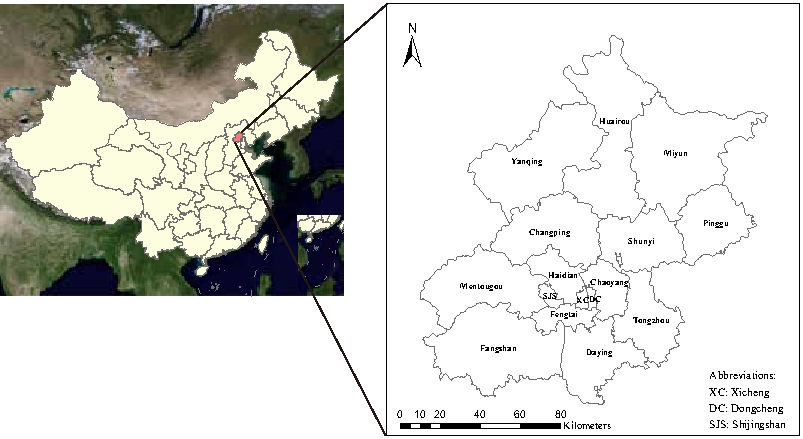
\includegraphics[width=\textwidth]{Figures/StudyArea.pdf}
    \caption{Location map and 16 administrative districts of Beijing}
    \label{fig:study_area}
\end{figure}

\subsection{Study area}
This study is conducted in the city of Beijing, the capital of China.
As shown in Figure \ref{fig:study_area}, Beijing locates at the North China Plain, occupying an area of 16,411km$^2$ (39.4{\degree}-41.6{\degree}N, 115.7{\degree}-117.4{\degree}E).
In 2019, the municipal population of Beijing have reached 21.53 million. According to Beijing Health Commission, 352 confirmed cases\footnote{\url{http://wjw.beijing.gov.cn/xwzx_20031/wnxw/202002/t20200212_1628835.html} (in Chinese)} were found in Beijing by February 10, 2020.
As a population-importing metropolis, Beijing has taken measures in response to the outbreak. 
Under this circumstance, the activities of residents have been influenced and showing special spatiotemporal patterns different from ordinary days.

\subsection{Data Sets}
\textbf{BSS spatiotemporal data} Temporal positioning datasets come from 900 thousand SBs belonging to 3 main BSS operators (Mobike, DiDi Bike, Hellobike and Ofo) in Beijing.
The datasets date from March 2018 to March 2020 (66.8 GB) and cover 1.5 million usage per day contributed by 11 million users which account for one half of the total population of Beijing.
Records of the datasets contain the positioning and timing information of locking \& unlocking bikes, excluding that of rebalancing operations.
This feature suggests that the movement of bikes are done by users.
Certain districts (Chaoyang, Fengtai and Shijingshan) are not comprised in the datasets due to different policies of local governments.

\textbf{Points Of Interest (POIs)} POIs of Beijing are collected from AutoNavi API\footnote{\url{https://lbs.amap.com/api/webservice/guide/api/georegeo} (in Chinese)}.
Each entry is identified by \texttt{object\_id}, recording the address including longitude/latitude information, and categorized by \texttt{large\_category}, \texttt{mid\_category} and \texttt{sub\_category}.
Among hundreds of categories, we chose six mid ones characterizing productive and social activities: residential area (RA), tech company, other company, subway station, shopping plaza and supermarket.

\begin{figure}[ht]
    \centering
    \begin{subfigure}{.23\textwidth}
        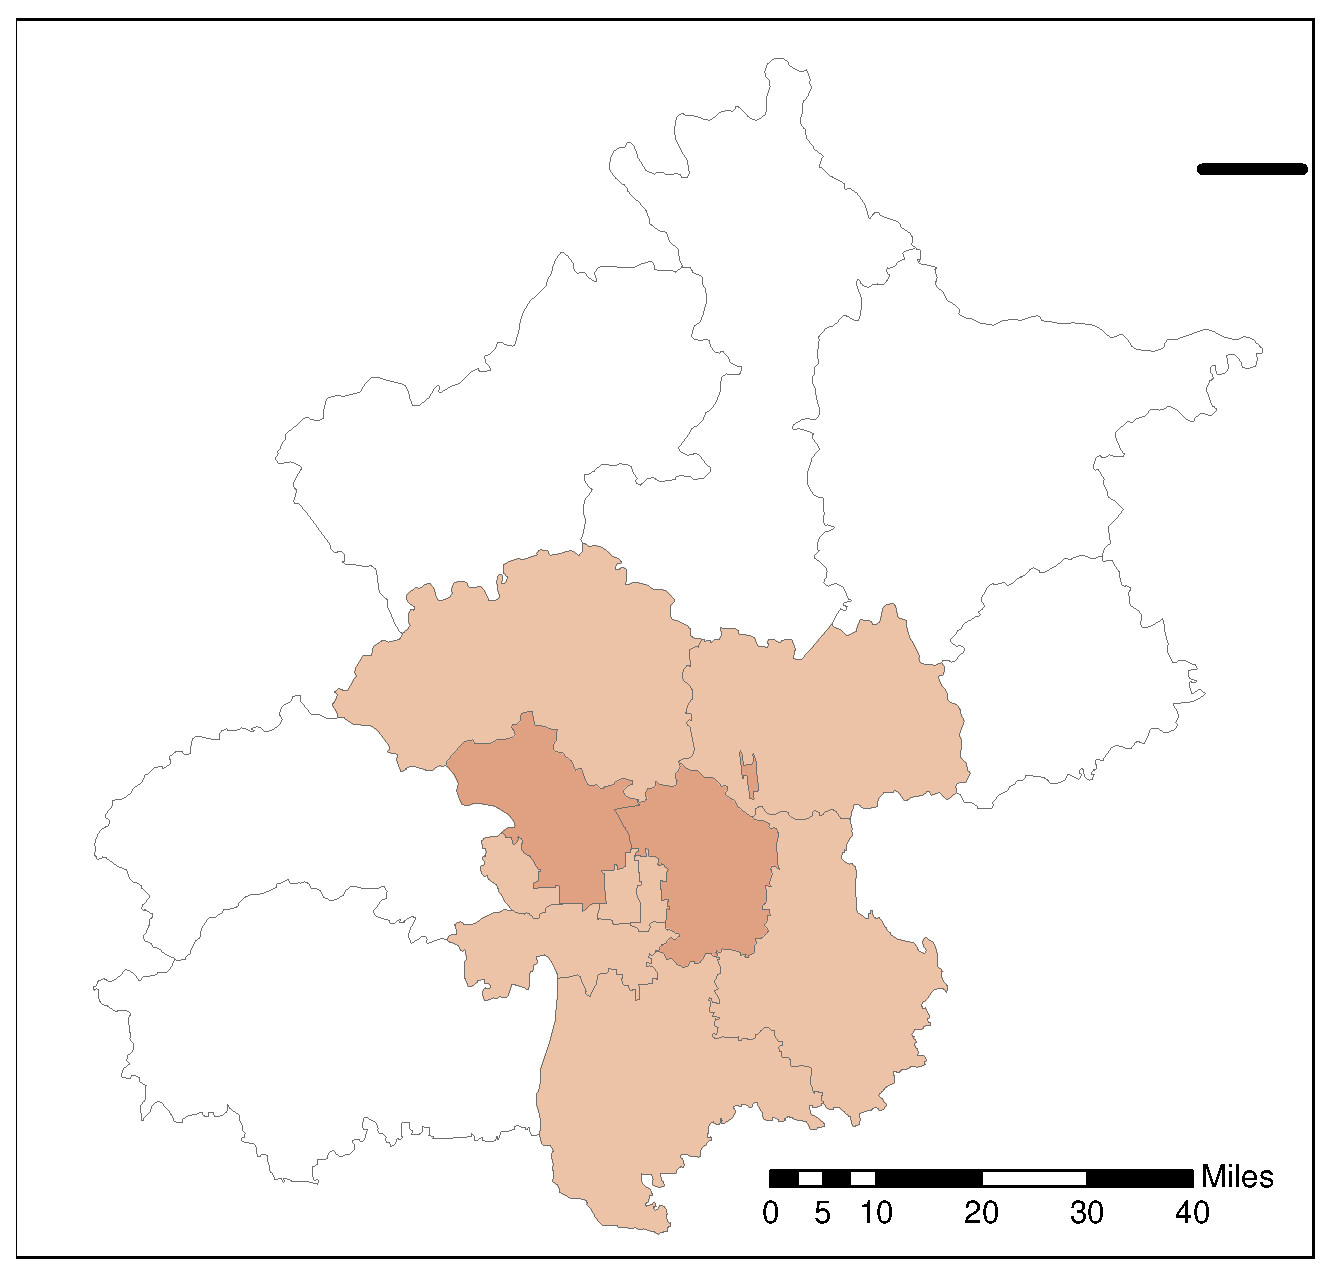
\includegraphics[width=\textwidth]{Figures/ConfirmedDistrictD2020_01_25.eps}
        \caption{25 Jan, 2020}
    \end{subfigure}
    \begin{subfigure}{.23\textwidth}
        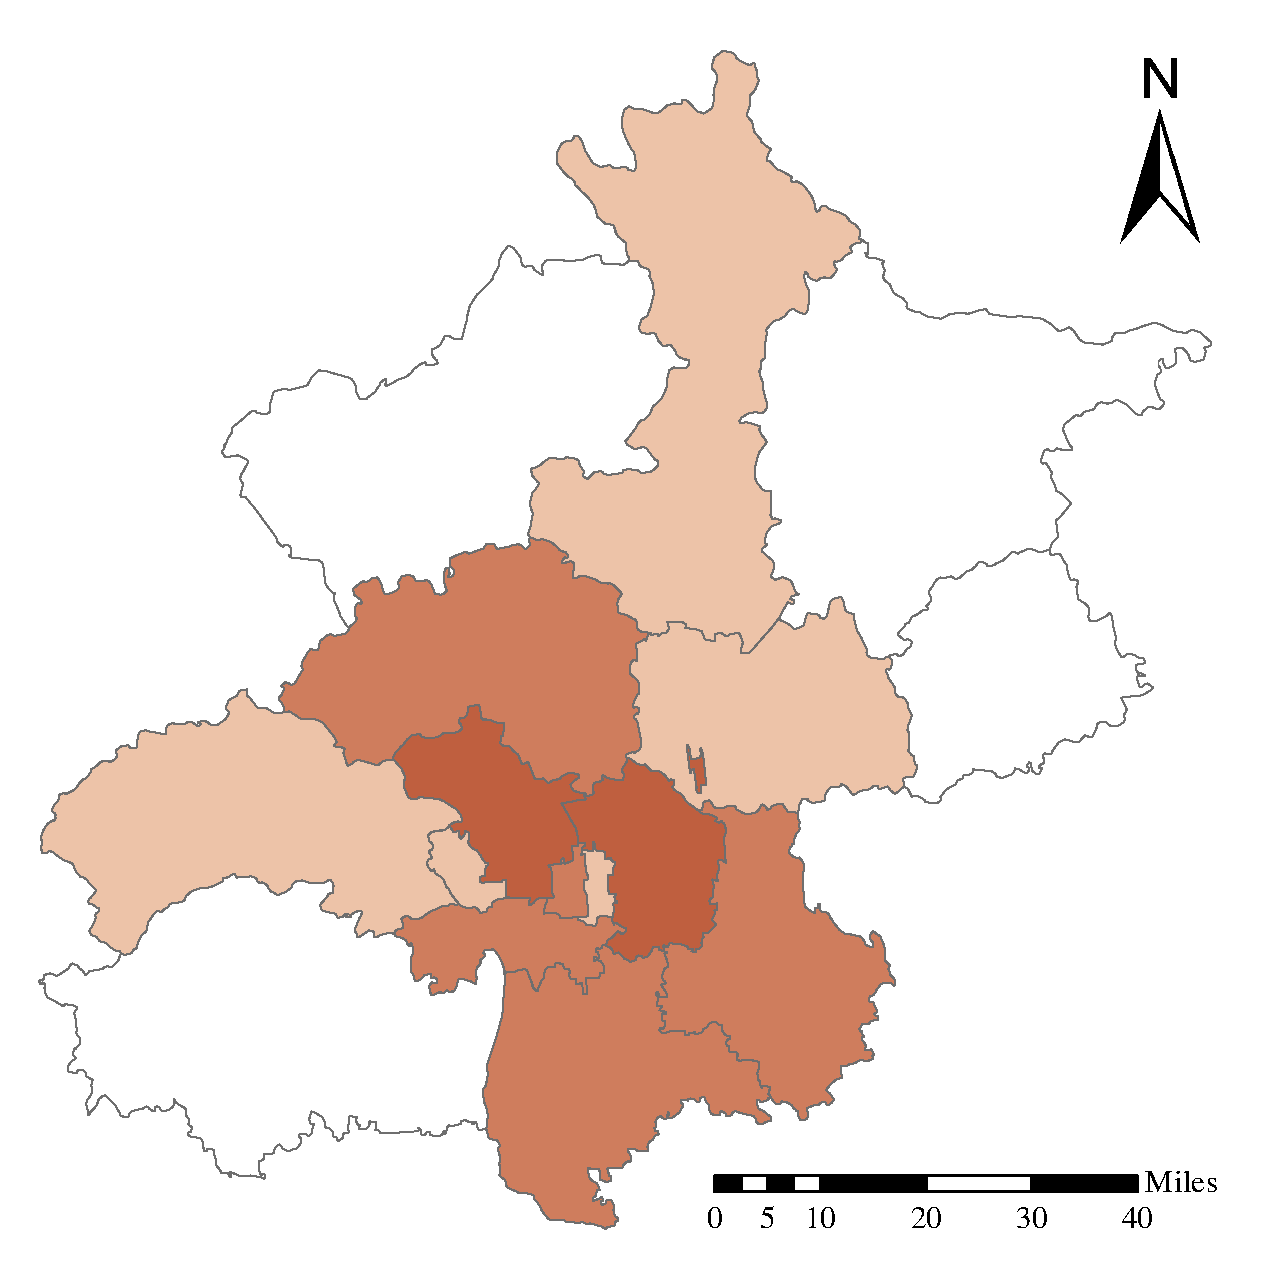
\includegraphics[width=\textwidth]{Figures/ConfirmedDistrictD2020_01_30.eps}
        \caption{30 Jan, 2020}
    \end{subfigure}
    \begin{subfigure}{.23\textwidth}
        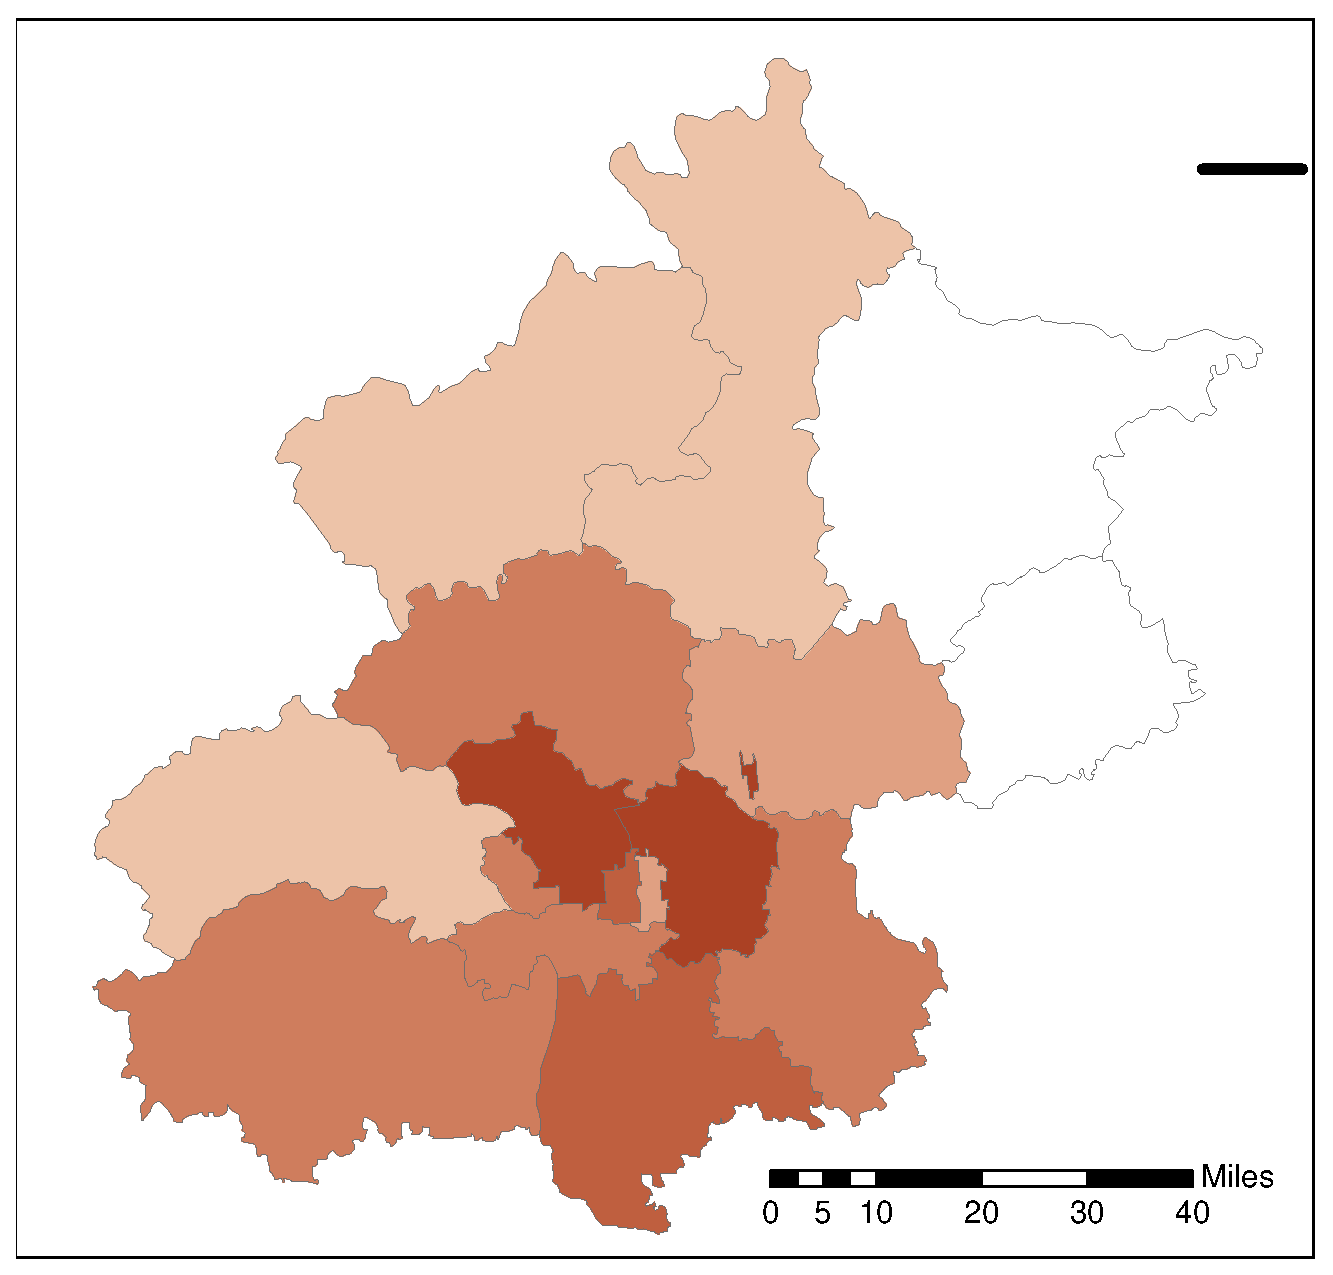
\includegraphics[width=\textwidth]{Figures/ConfirmedDistrictD2020_02_05.eps}
        \caption{05 Feb, 2020}
    \end{subfigure}
    \begin{subfigure}{.23\textwidth}
        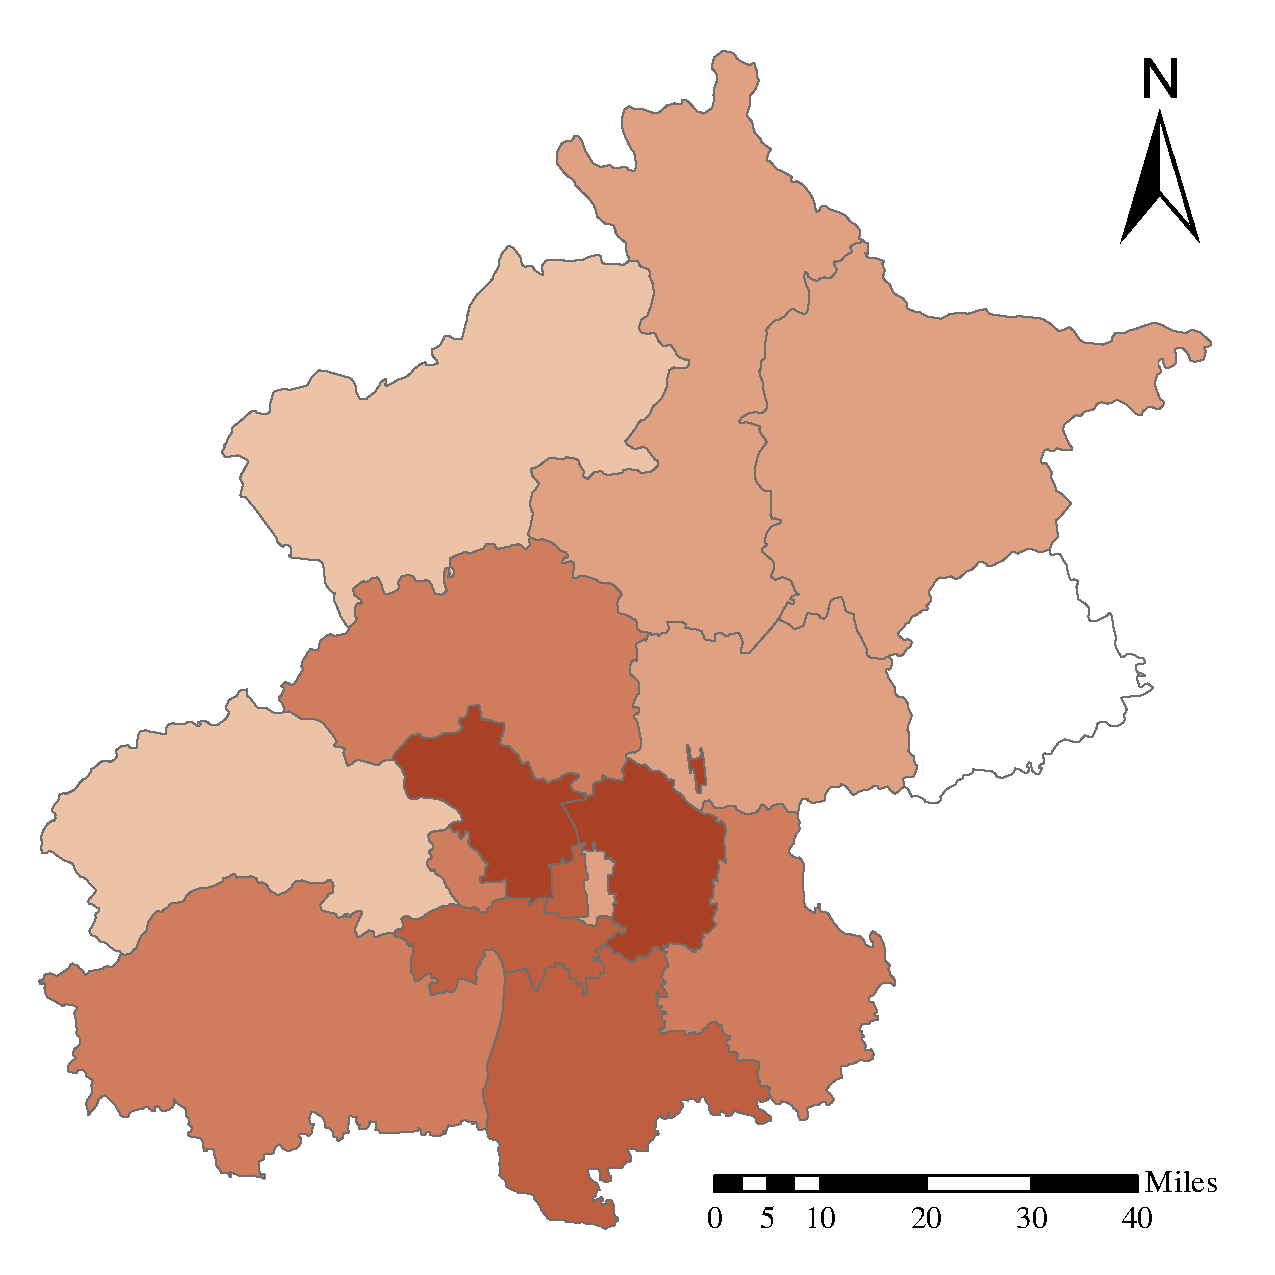
\includegraphics[width=\textwidth]{Figures/ConfirmedDistrictD2020_02_10.eps}
        \caption{10 Feb, 2020}
    \end{subfigure}

    \vspace{6pt}
    \begin{subfigure}{0.7\textwidth}
        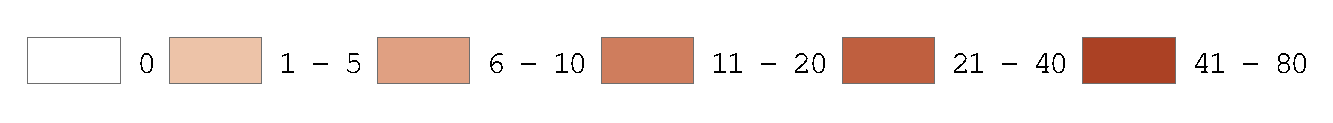
\includegraphics[width=\textwidth]{Figures/Fig2legend.eps}
    \end{subfigure}
    \caption{Daily counts of confirmed cases in Beijing}
    \label{fig:number_of_confirmed_cases}
\end{figure}

\textbf{Locations of Confirmed Cases}
The daily counts of confirmed 2019-nCoV cases subjected to each district from Jan 20 to Mar 5, 2020 were collected from the daily update on the novel coronavirus pneumonia outbreak dashboard provided by National Health Commission of the People's Republic of China\footnote{\url{http://www.nhc.gov.cn/xcs/yqtb/list_gzbd.shtml} (in Chinese)} .
According to the timeline \cite{li2020early} of the outbreak, we picked several important dates shown in Figure \ref{fig:number_of_confirmed_cases}, visualizing the evolution of the overall pandemic situation of Beijing.
To assess the overall behavior pattern changes, we picked out the locations of infected RAs (see Figure \ref{fig:locations_of_confirmed_cases}), which were retrieved from Beijing Municipal Health Commission\footnote{\url{http://wjw.beijing.gov.cn/xwzx_20031/wnxw/202003/t20200305_1679143.html} (as of March 05, 2020, in Chinese)}.  

\begin{figure}[ht]
    \centering
    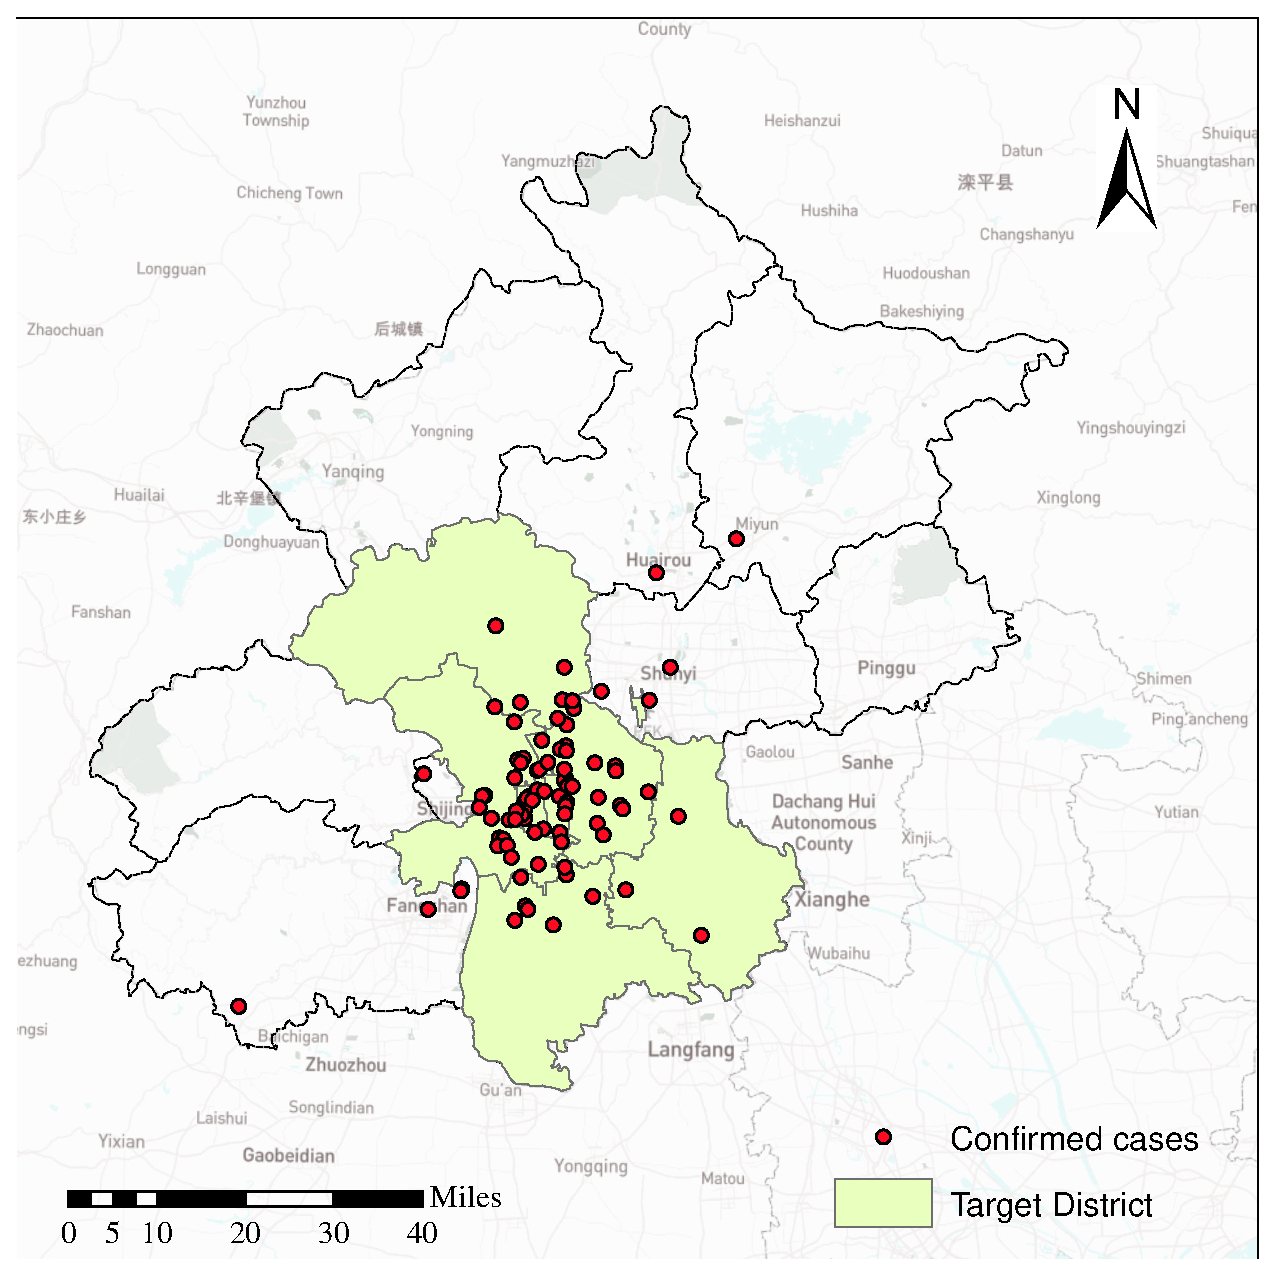
\includegraphics[width=.5\textwidth]{Figures/Plot_location_confirmed_cases.eps}
    \caption{Locations of confirmed cases in Beijing}
    \label{fig:locations_of_confirmed_cases}
\end{figure}

\section{Tools and Methods}

\subsection{Parallel Computing}
Traditional geospatial tools such as PostGIS, QGIS are no longer able to deal with large-scale spatial queries huge amount of BSS spatiotemporal data (66.8GB) due to limited of computer performance stand-alone machine.
To obtain the co-location patterns in such datasets with numerous POIs, we proceeded with GeoSpark SQL \cite{huang2017geospark}, which performs spatial queries via parallel computing on cluster computing framework Spark\footnote{\url{https://spark.apache.org/}}.
Among the spatial queries, we utilized \texttt{spatial\_join(geom1, geom2)}, querying if \texttt{geom1} is inside \texttt{geom2} and \texttt{distance\_join(geom1, geom2, dist)} querying if the distance of \texttt{geom1} and \texttt{geom2} is less than \texttt{dist}.
These queries are nearly partition independent, recomputing is needed only on the borders of partition, thus our parallel efficiency is high given proper configuration and partitioning.

\subsection{Phase Classification}\label{sec:phase_classification}
In machine learning, it is often demanded to minimize the predefined loss function to perform the best classification such that elements within the same cluster are similar and elements across clusters are different.

Likewise, we try to divide the study period into phases which have resembling share bike usage.

\begin{Definition}[k-segmentation]
Let $X=\{x_1,x_2,\ldots,x_N\}$ be a time series of length $N$.
Given positive integer $k<N$ and index set $\mathbf{T}=\{n_0,\ldots,n_k\}$ with $n_0=0$, $n_k=N$ and $\forall i$, $n_i<n_{i+1}$, a k-segmentation of $X$ is the set of time series $X_i=\{x_{n_i+1},\ldots,x_{n_{i+1}}\}$ where $0\leq i\leq k-1$.
\end{Definition}

To evaluate the quality of k-segmentation, we use $\sigma=\sum_{i=1}^{k}{\sigma_i}$ as loss function where $\sigma_i$ is the standard deviation of division $X_i$. 
The goal is to find the best $T$ to minimize $\sigma$, \textit{i.e.} $\arg\min_{\mathbf{T}}\sigma(\mathbf{T})$.
This problem is solved in time $O(N^2k)$ \cite{terzi2006efficient}.
In case $k$ and $N$ are small, the optimum can be found via exhaustive search.

\subsection{Basic statistics}
The evolution of share bike usage over time in different zones of Beijing, as well as their relationships with COVID-19 spreading status and facilities, are the focus of this research.
To obtain these results, spatial analysis and statistics are implemented in Python with the help of ESRI ArcGIS 10.7. 

\section{Result}

\subsection{Temporal patterns of cycling activities}
To better characterize the behavior patterns with respect to the COVID-19 epidemic dynamics, we first selected the following important referential dates in Table \ref{tab:important_dates} that could affect the virus transmission in Beijing: 

\begin{table}[ht]
    \centering
    \begin{tabular}{ll}
    04 Feb 2019 & Start of Chinese New Year holiday 2019\\
    10 Feb 2019 & End of new year holiday 2019\\
    07 Jan 2020 & Identification of COVID-19\\
    22 Jan 2020 & Shut down of Wuhan and other 15 cities\\
    24 Jan 2020 & Start of Chinese New Year holiday 2020\\
    02 Feb 2020 & End of \textit{extended} New Year holiday 2020\\
    10 Feb 2020 & Partial restart of productive and social activities
    \end{tabular}
    \caption{Important dates}
    \label{tab:important_dates}
\end{table}

As the outbreak of COVID-19 coincides with Chinese New Year holiday 2020, we use Chinese New Year holiday of 2019 as comparison to assess the influence of this period on share bike usage.
It is worth noticing that Chinese New Year holidays are not equi-length, especially that of 2020, which is extended by executive order.

We compared the share bike usage on rush hours (8:00-09:00) during a period of 64 days from 01 Jan to 02 March 2019 and 01 Jan to 01 March 2020 respectively (data of 29 Feb and 1 March 2020 were brought backward by one day due to the leap year 2020).
% As can be seen in Figure \ref{fig:temporal_comparison}, in 2019, the usage drops down to $5\times 10^5$ because of Chinese New Year holiday; 
% while in 2020, the usage decreases even two thirds of that in 2019 due to the outbreak of COVID-19 and the following epidemics.

% \begin{figure}[ht]
%     \centering
%     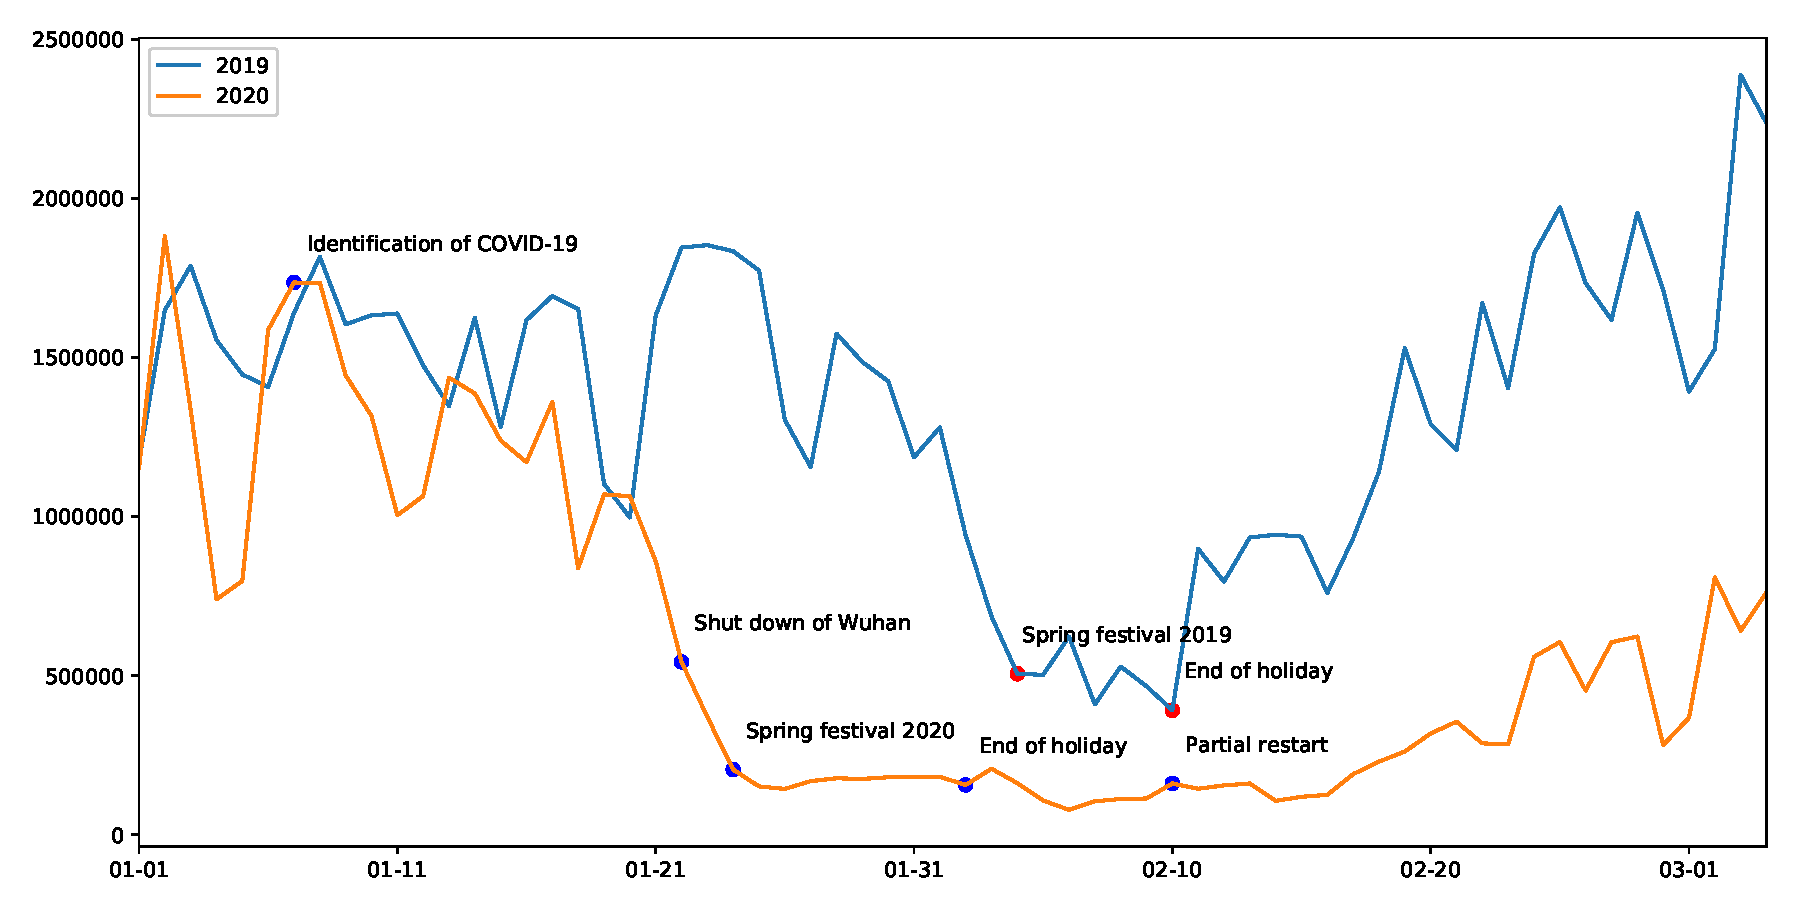
\includegraphics[width=\textwidth]{Compare_temporal.eps}
%     \caption{Comparison between share bike daily usage of year 2019 and 2020.}
%     \label{fig:temporal_comparison}
% \end{figure}

Figure \ref{fig:hour_comparison_8} % and Figure \ref{fig:hour_comparison_18}
 illustrate the temporal evolution of share bike usage.

\begin{figure}[ht]
    \centering
    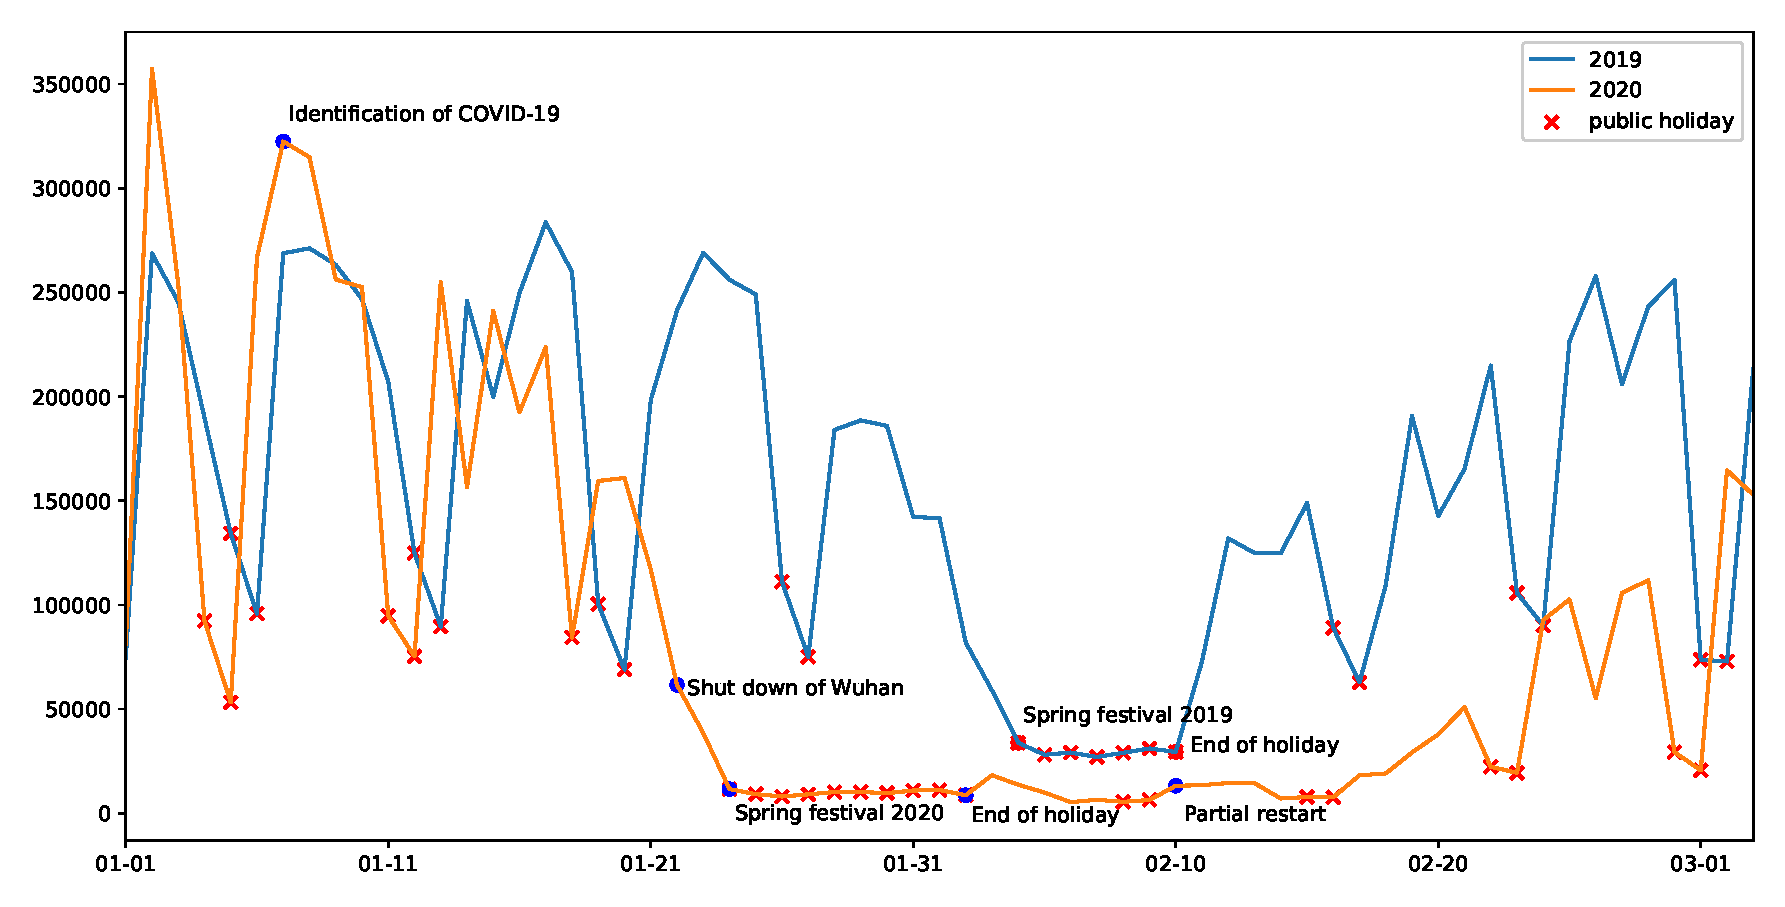
\includegraphics[width=0.9\textwidth]{Figures/hour_8.eps}
    \caption{share bike usage during 08:00-09:00 of year 2019 and 2020.}
    \label{fig:hour_comparison_8}
\end{figure}
% \begin{figure}[ht]
%     \centering
%     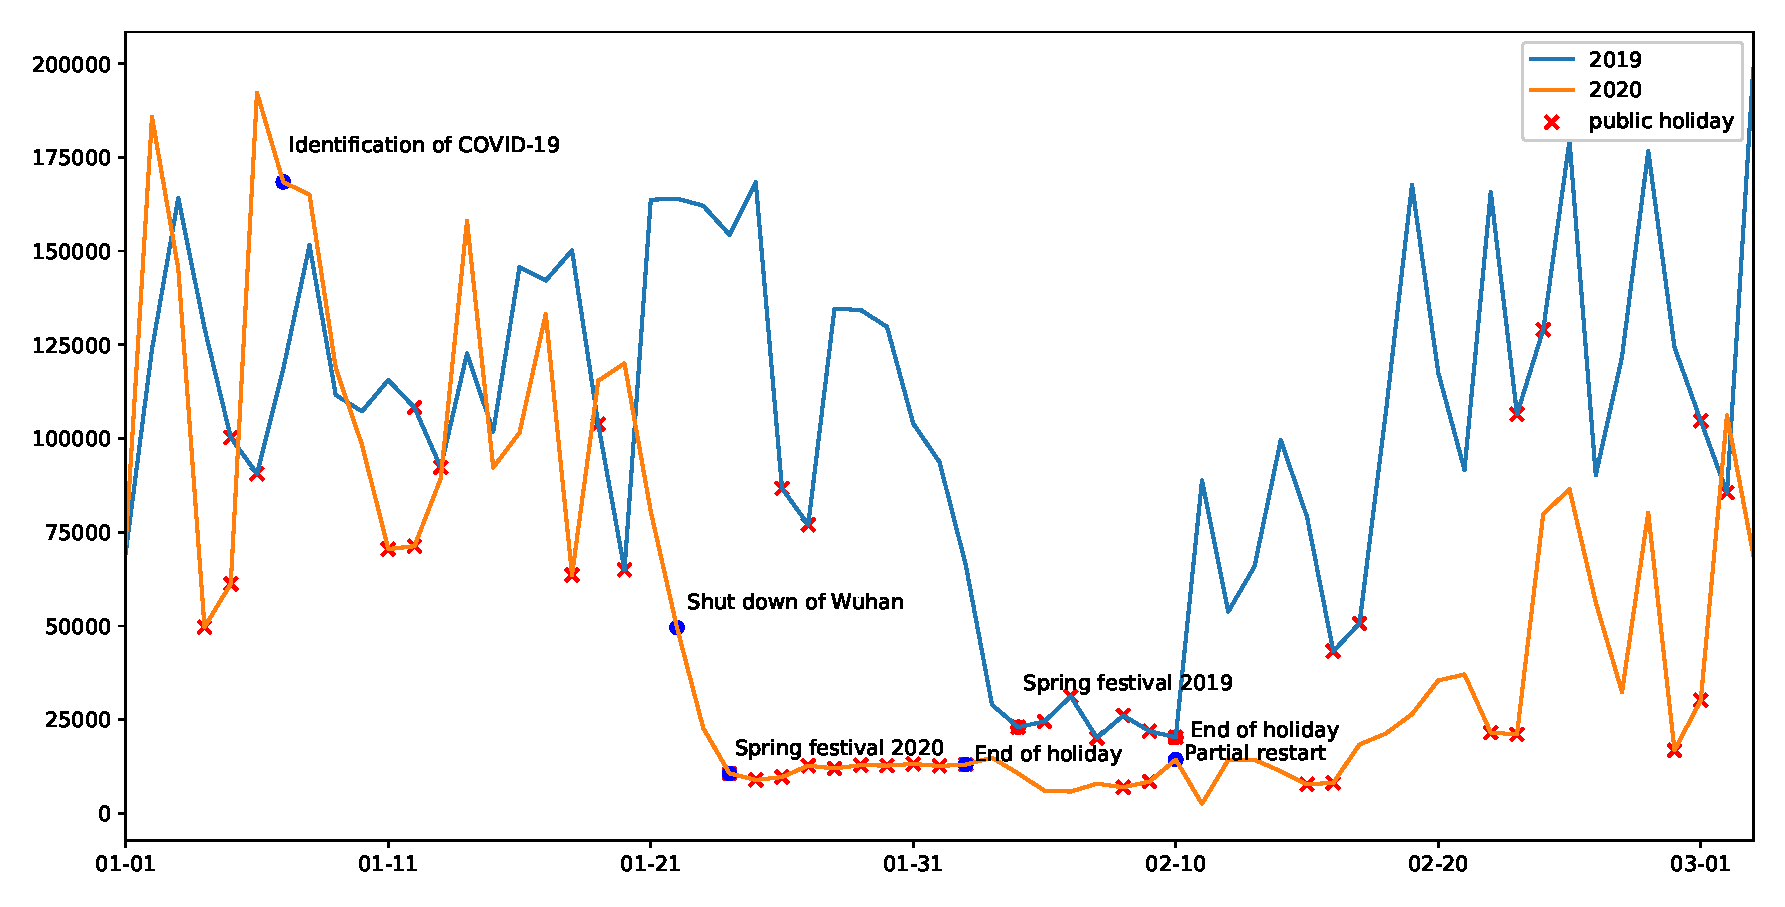
\includegraphics[width=0.9\textwidth]{Figures/hour_18.eps}
%     \caption{share bike usage during 18:00-19:00 of year 2019 and 2020.}
%     \label{fig:hour_comparison_18}
% \end{figure}

The share bike usage drops in mid-January of 2020 and early February of 2019.
During these periods, schools and workplaces were closed as part of the Chinese New Year holiday 2020.
The overall closure was then forced to be extended to mitigate the pandemic.

% We also plotted the graph of share bike usage during rush hour (8:00-10:00 and 18:00-20:00) which reflects the productive activities.
share bike usage on rush hours exhibits the periodicity of productive activities: high on weekdays and low on weekends, which fits our general knowledge.
However, this pattern does not appear on 10 Feb 2020 when the government declared the partial restart of certain productive and social activities.
This anomaly suggests that the activities were not resumed at all until Feb 17, one week after the partial restart, corresponding to the fact that the impact of the pandemic was lasting till the end of our study period.

Table \ref{tab:overall_comparison} gives a rough quantitative view over the impact of the pandemic.

\textbf{Note:} In this paper, we consider share bike usage follows normal distribution, of which $95\%$ confidence interval is $[\bar{x}-2\sigma,\bar{x}+2\sigma]$.
Share bike usage data are presented in the form $\bar{x}\pm2\sigma$.

\begin{table}[ht]
    \centering
    \begin{tabular}{|l|l|l|l|}
        \hline
        \multirow{2}{*}{Phase} &\multicolumn{3}{c|}{Daily average share bike usage ($10^{5}$)}\\
        \cline{2-4}
        & 08:00-09:00 (weekday) & 18:00-19:00 (weekday) & All-day\\
        \hline
        02 Jan-20 Jan 2019 & $2.46\pm0.59$ & $1.30\pm0.39$ & $15.0\pm4.5$\\
        \hline
        02 Jan-20 Jan 2020 & $2.58\pm1.10$ & $1.37\pm0.74$ & $12.7\pm6.3$\\
        \hline
        \hline
        04 Feb-10 Feb 2019 & $0.30\pm0.05$ & $0.24\pm0.08$ & $4.90\pm1.56$\\
        \hline
        24 Jan-02 Feb 2020 & $0.10\pm0.02$ & $0.12\pm0.03$ & $1.72\pm0.35$\\
        \hline
    \end{tabular}
    \caption{Overall comparison of year 2019 and 2020}\label{tab:overall_comparison}
\end{table}

The upper part shows in ordinary days, share bike usage in 2020 in on the same level of that of 2019, suggesting share bike demand is evolving in a smooth way.
However, the lower part shows the case of Chinese New Year holiday, overall share bike usage drops to less than 40\% compared with the same period in 2019, suggesting companies stopped working due to Chinese New Year holiday like the case of 2019, and social activities also halted. 

\subsection{Co-location Analysis with POIs}\label{sec:colo-poi}

From the previous section, it is implied the dates in Table \ref{tab:important_dates} may not be the optimal boundaries of different phases, for example Feb 17 does not appear.
We computed the best phase classificationm using definition in Section \ref{sec:phase_classification}.
We classified the period into three phases: before pandemics, during pandemics, pandemics mitigated.
Here $k=3$ and $N=64$, we found the best classified phases using exhaustive search and assign them with reasonable explanations: 01 Jan-21 Jan (before the pandemic), 22 Jan-16 Feb (critical phase of the pandemic) and 17 Feb-01 Mar (epidemics mitigated).
We computed then the BS usage in these phases.

\begin{table}[ht]
    \centering
    \begin{tabular}{|l|l|l|l|l|l|l|}
        \hline
        \multirow{2}{*}{Category} & \multirow{2}{*}{\makecell[c]{POI\\amount}} & \multicolumn{5}{c|}{Daily average bike usage within 200m radius of POIs per POI}\\
        \cline{3-7}
        & & 01 Jan-21 Jan ($a$) & 22 Jan-16 Feb ($b$) & 17 Feb-02 Mar ($c$) & $b/a$ & $c/a$\\ %$a/m$\\
        \hline
        RA & $5657$ & $158.3\pm86.9$ & $36.6\pm14.4$ & $39.9\pm13.9$ & $23.1\%$ & $25.2\%$\\ %$109.0\%$\\
        \hline
        Tech company & $3858$ & $200.4\pm112.9$ & $36.3\pm14.4$ & $41.1\pm18.0$ & $18.1\%$ & $20.5\%$\\ %$113.2\%$\\
        \hline
        Other company & $32301$ & $162.5\pm90.3$ & $35.8\pm14.5$ & $39.4\pm14.5$ & $22.0\%$ & $24.2\%$\\ %$110.1\%$\\
        \hline
        Subway station & $137$ & $113.8\pm66.6$ & $29.0\pm11.8$ & $31.7\pm10.6$ & $25.5\%$ & $27.9\%$\\ %$109.3\%$\\
        \hline
        Shopping plaza & $217$ & $168.9\pm91.7$ & $38.4\pm14.6$ & $41.0\pm15.0$ & $22.7\%$ & $24.3\%$\\ %$106.8\%$\\
        \hline
        Supermarket & $1076$ & $137.6\pm76.0$ & $34.3\pm13.4$ & $37.7\pm13.6$ & $24.9\%$ & $27.4\%$\\ %$109.9\%$\\
        \hline
    \end{tabular}
    \caption{Bike usage in different phases around the chosen POIs.
    %, where $c=(b+a)/2m$ is used to measure the bending of the evolution curve
    }
    \label{tab:bike_usage_poi}
\end{table}

Table \ref{tab:bike_usage_poi} depicts the bike usage of the six chosen categories.
Phase $a$ and $b$ have the same duration, 21 days.     
% In abuse of definition ``convexity'', we use the comparison between the mean of $a$ and $b$ and phase $m$ (mid) to describe the curve: the curve is more bending, \textit{\textit{i.e.}} impacted if ratio $c=(b+a)/2m$ is larger.
Ratio $b/a$ shows that the bike usage of all categories decreased to one quarter, and tech companies dropped the most in both value and proportion, one possible explanation is they suit best ``work from home''. 
Ratio $c/a$ shows the bike usage of all categories have recovered to some extent but far from the situation of usual time after the partial restart of activities.

As can be inferred in Figure \ref{fig:BSS_metro} and Figure \ref{fig:BSS_malls} in Appendix, metro stations and malls always position in the center of massive share bike clusters.
In Figure \ref{fig:BSS_companies}, tech companies are crowded in the northwest of Beijing which take the biggest BS usage.
However, the mobility does not recover even after the pandemic was mitigated.

\subsection{Co-location Analysis with Infected RAs}

From Figure \ref{fig:locations_of_confirmed_cases}, we noticed that, being the center of Beijing, Dongcheng and Xicheng district contain most of the infected RAs, and the confirmed time lie between 05 and 12 February.
Like in Section \ref{sec:colo-poi}, we adjusted the time intervals to match the confirmed time and carried the same snalysis on the share bike usage around infected RAs and that of surrounding RAs (within the range of 1500m of infected RAs).

\begin{table}[ht]
    \centering
    \begin{tabular}{|l|l|l|l|l|l|l|}
        \hline
        \multirow{2}{*}{Category} & \multirow{2}{*}{\makecell[c]{RA\\amount}} & \multicolumn{5}{c|}{Daily average bike usage within 200m radius of RAs per RA}\\
        \cline{3-7}
        & & 01 Jan-21 Jan ($a$) & 05 Feb-12 Feb ($b$) & 13 Feb-04 Mar ($c$) & $b/a$ & $c/a$\\
        \hline
        Infected RA & $19$ & $160.8\pm99.4$ & $27.3\pm22.7$ & $43.2\pm32.6$ & $17.0\%$ & $26.9\%$\\%158.2\% \\
        % Infected RA & 19 & 181.3 & 41.1 & 26.5 &  & \\
        \hline
        Surrounding RA & $1591$ & $139.2\pm84.4$ & $26.8\pm20.1$ & $38.7\pm26.1$ & $19.3\%$ & $27.8\%$\\% 144.4\%\\
        \hline
        All RA & $5657$ & $158.3\pm86.9$ & $36.6\pm14.4$ & $39.9\pm13.9$ & $23.1\%$ & $25.2\%$\\% 119.0\%\\
        \hline
    \end{tabular}
    \caption{Bike usage in different phases of infected RAs and that of surrounding RAs.}
    \label{tab:bike_usage_infected}
\end{table}

From Table \ref{tab:bike_usage_infected}, it can be inferred that the infected RAs suffered the most among the listed categories according to ratio $b/a$.
Strict quarantine was practised here to mitigate the pandemic.
Surrounding RAs were also strongly impacted because of the residents got into panic and keep themselves at home.
According to ratio $c/a$, the share bike usage of infected RAs and their surrounding RAs have recovered roughly to the same level compared to other RAs from the pandemic.

As can be seen from the BS usage of 16 Jan in Figure \ref{fig:BSS_communities}, the infected RAs are actually situated in the city center, with huge pedestrian flow rate surrounded by massive SBs.
On 15 Feb, there is nearly no share bike usage around these infected RAs.
On 2 Mar, nearly no massive share bike usage can be observed around the infected RAs, unlike metro stations and shopping plazas.

We can conclude the residents in Beijing followed exactly the suppression strategy whether the RAs were infected or not: quarantine, \textit{cordon sanitaire} and social distancing.

\subsection{Spatiotemporal patterns of cycling activities}

\begin{figure}[ht]
    \centering
    \begin{subfigure}{.23\textwidth}
        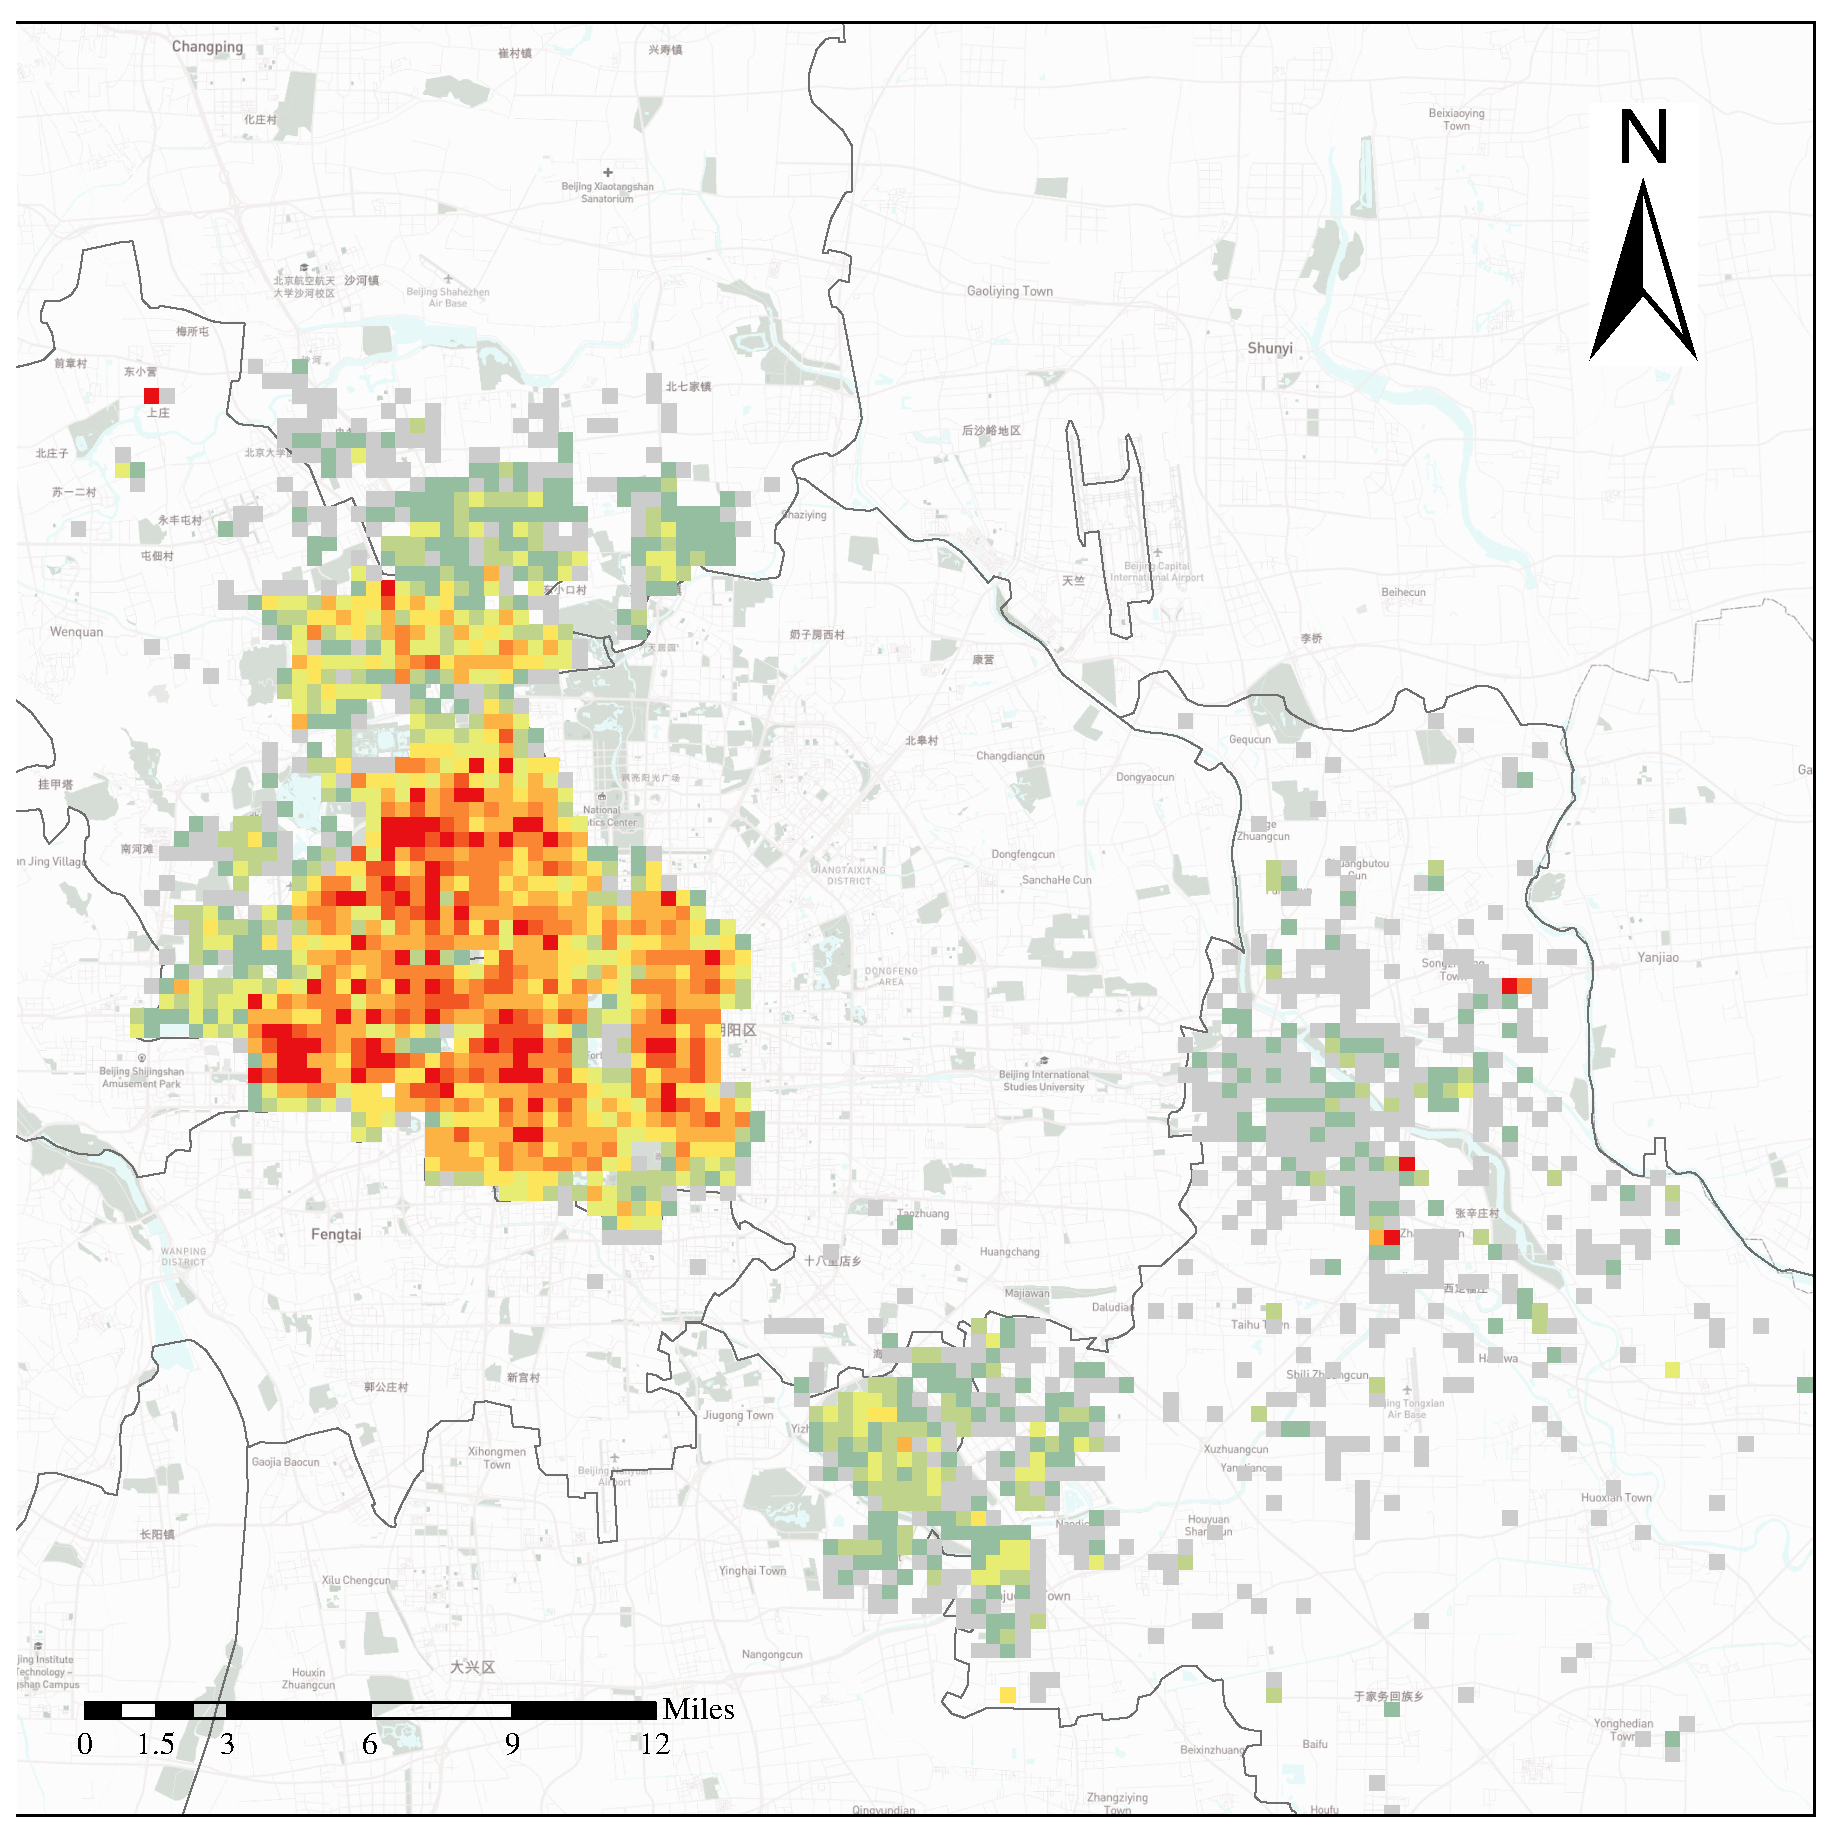
\includegraphics[width=\textwidth]{Figures/Overall_spatial_patterns/FN5_D2020_01_21.eps}
        \caption{21 Jan}
    \end{subfigure}
    \begin{subfigure}{.23\textwidth}
        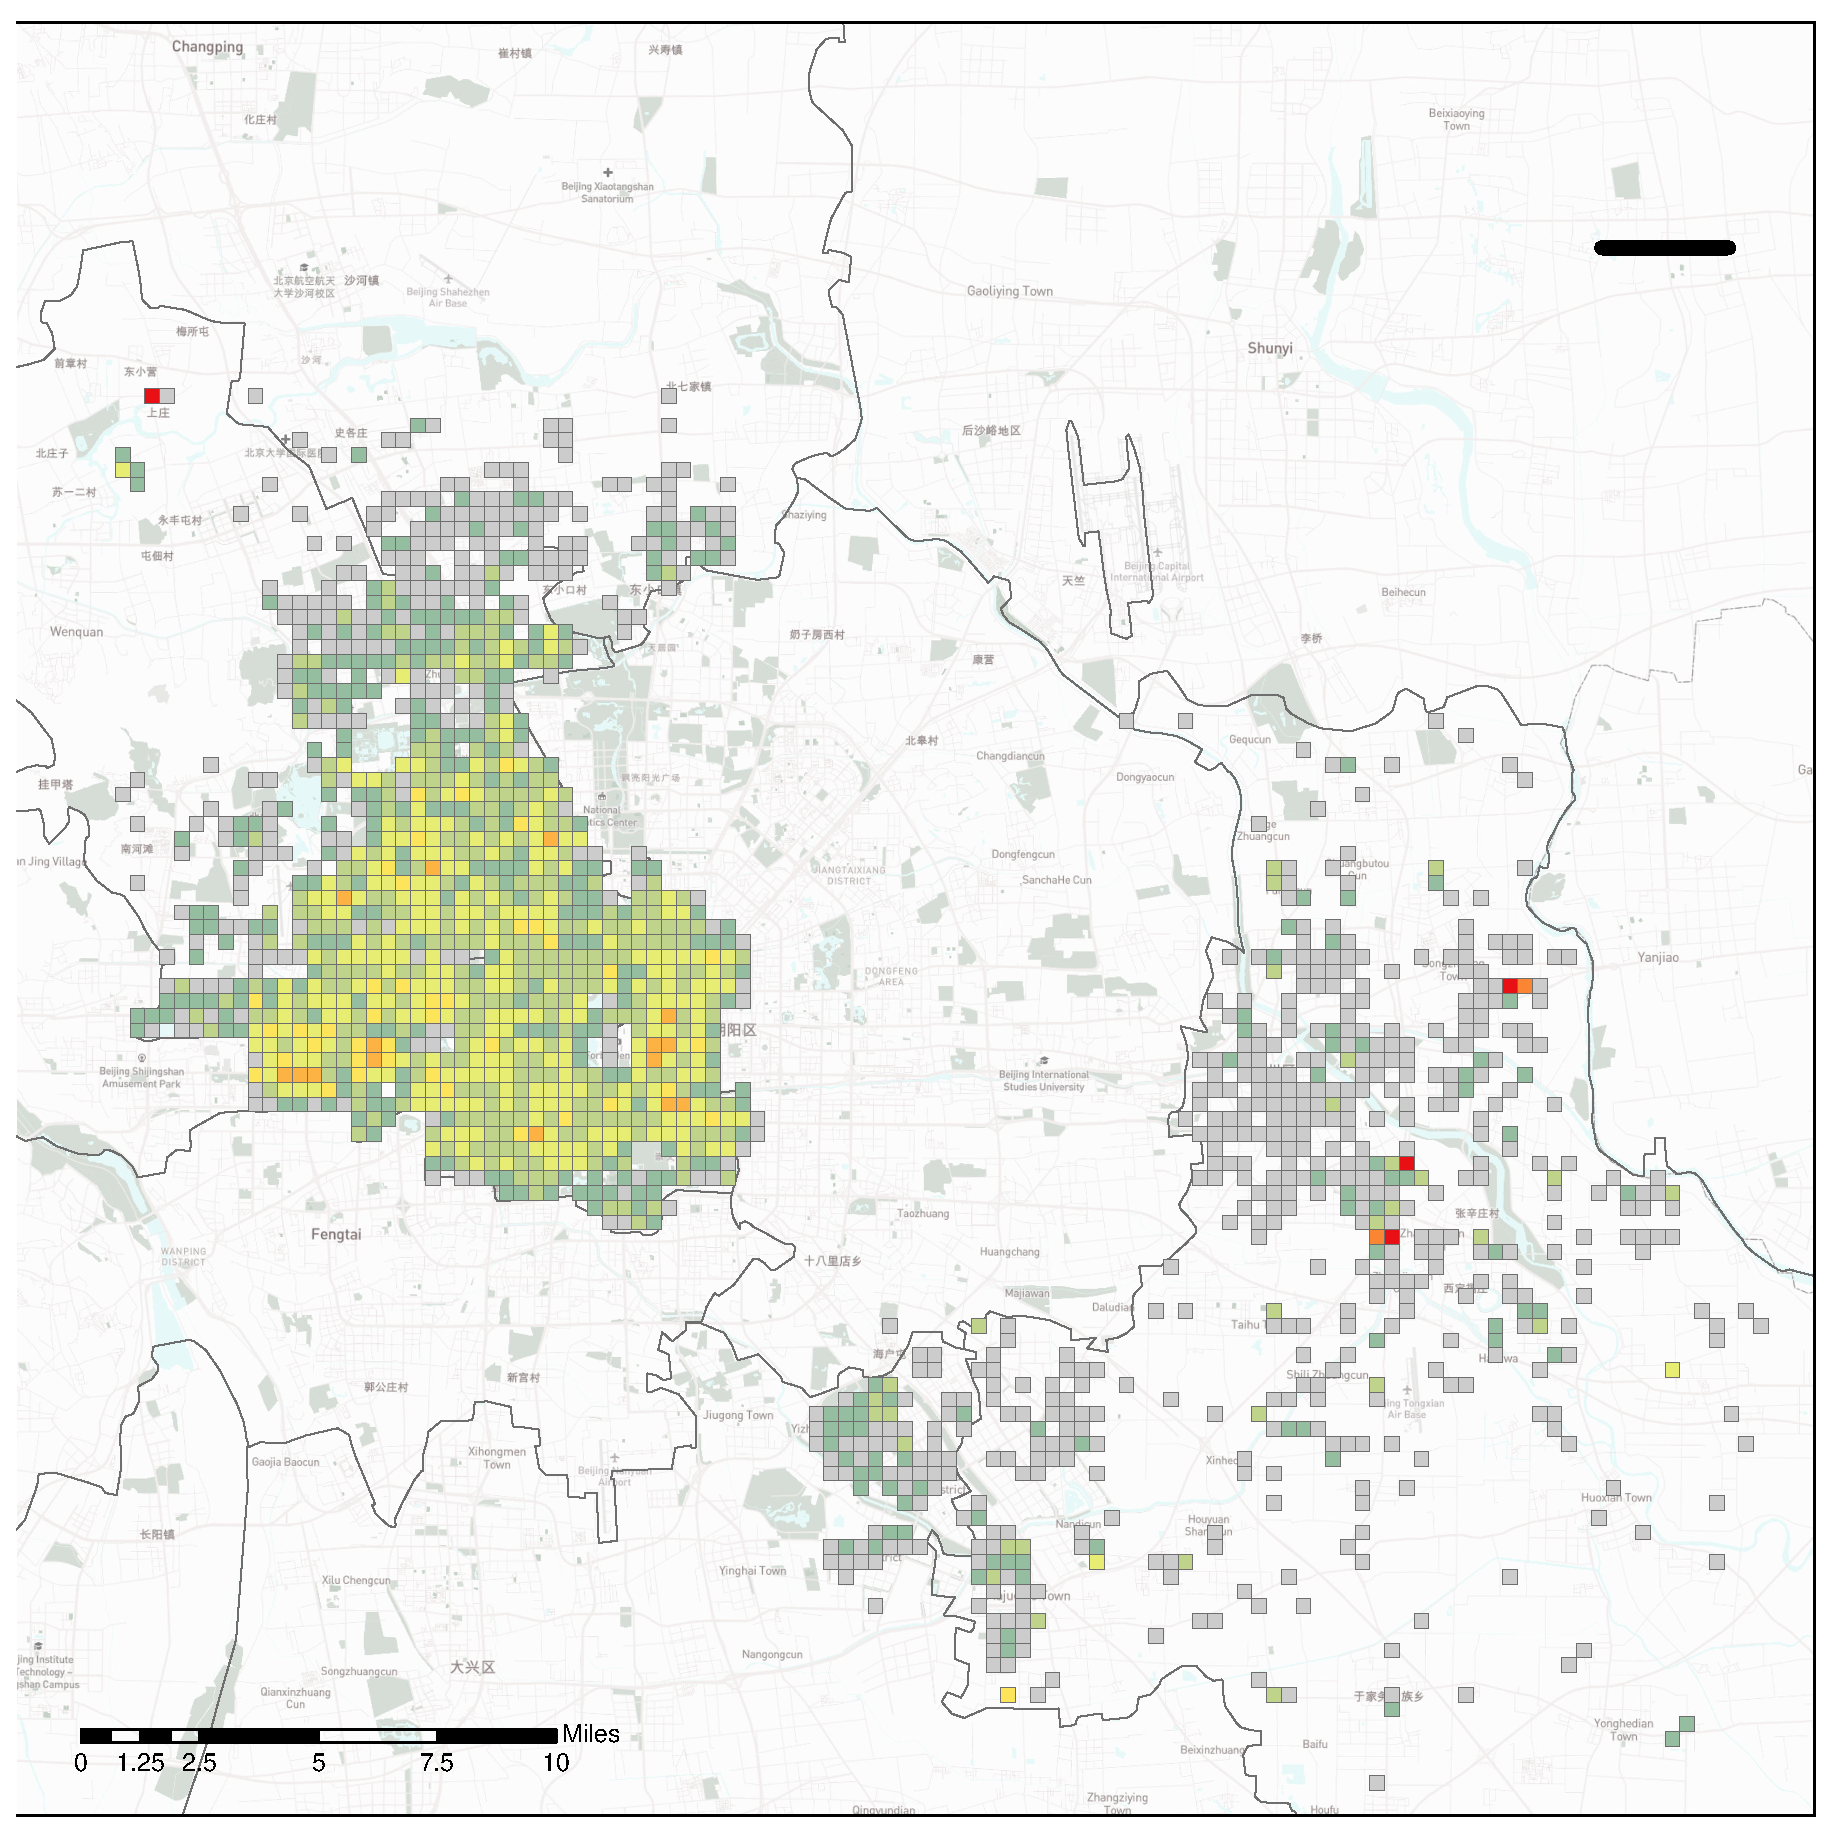
\includegraphics[width=\textwidth]{Figures/Overall_spatial_patterns/FN5_D2020_01_25.eps}
        \caption{25 Jan}
    \end{subfigure}
    \begin{subfigure}{.23\textwidth}
        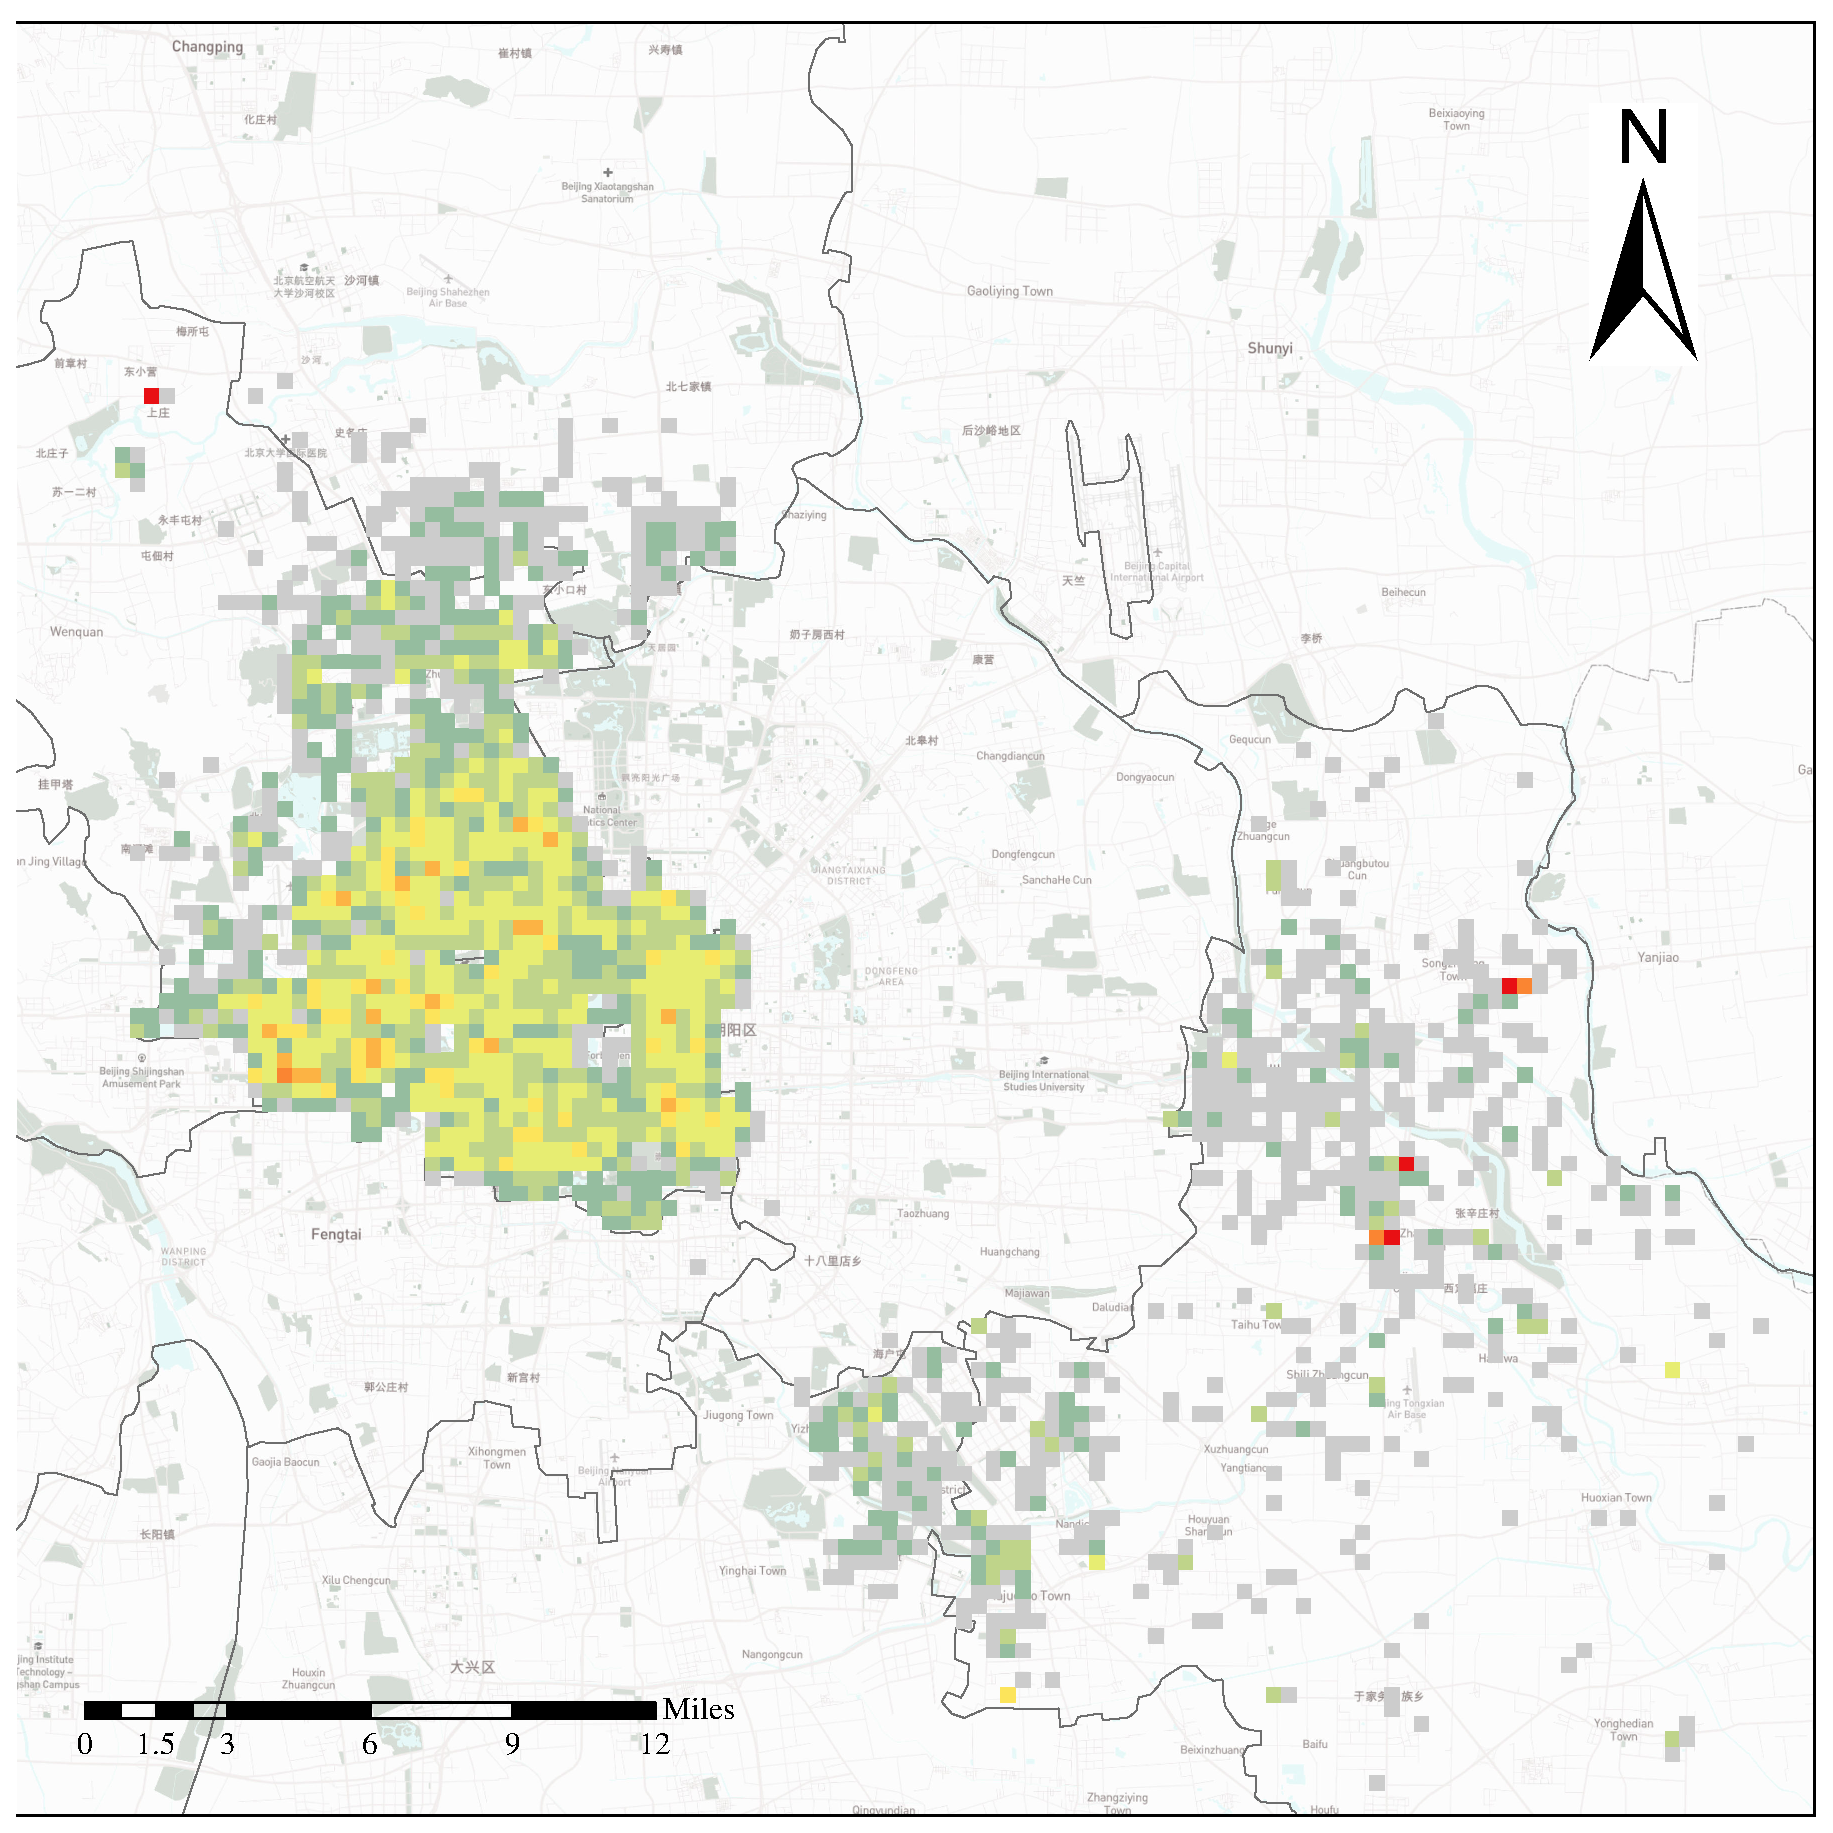
\includegraphics[width=\textwidth]{Figures/Overall_spatial_patterns/FN5_D2020_01_29.eps}
        \caption{29 Jan}
    \end{subfigure}
        \begin{subfigure}{.23\textwidth}
        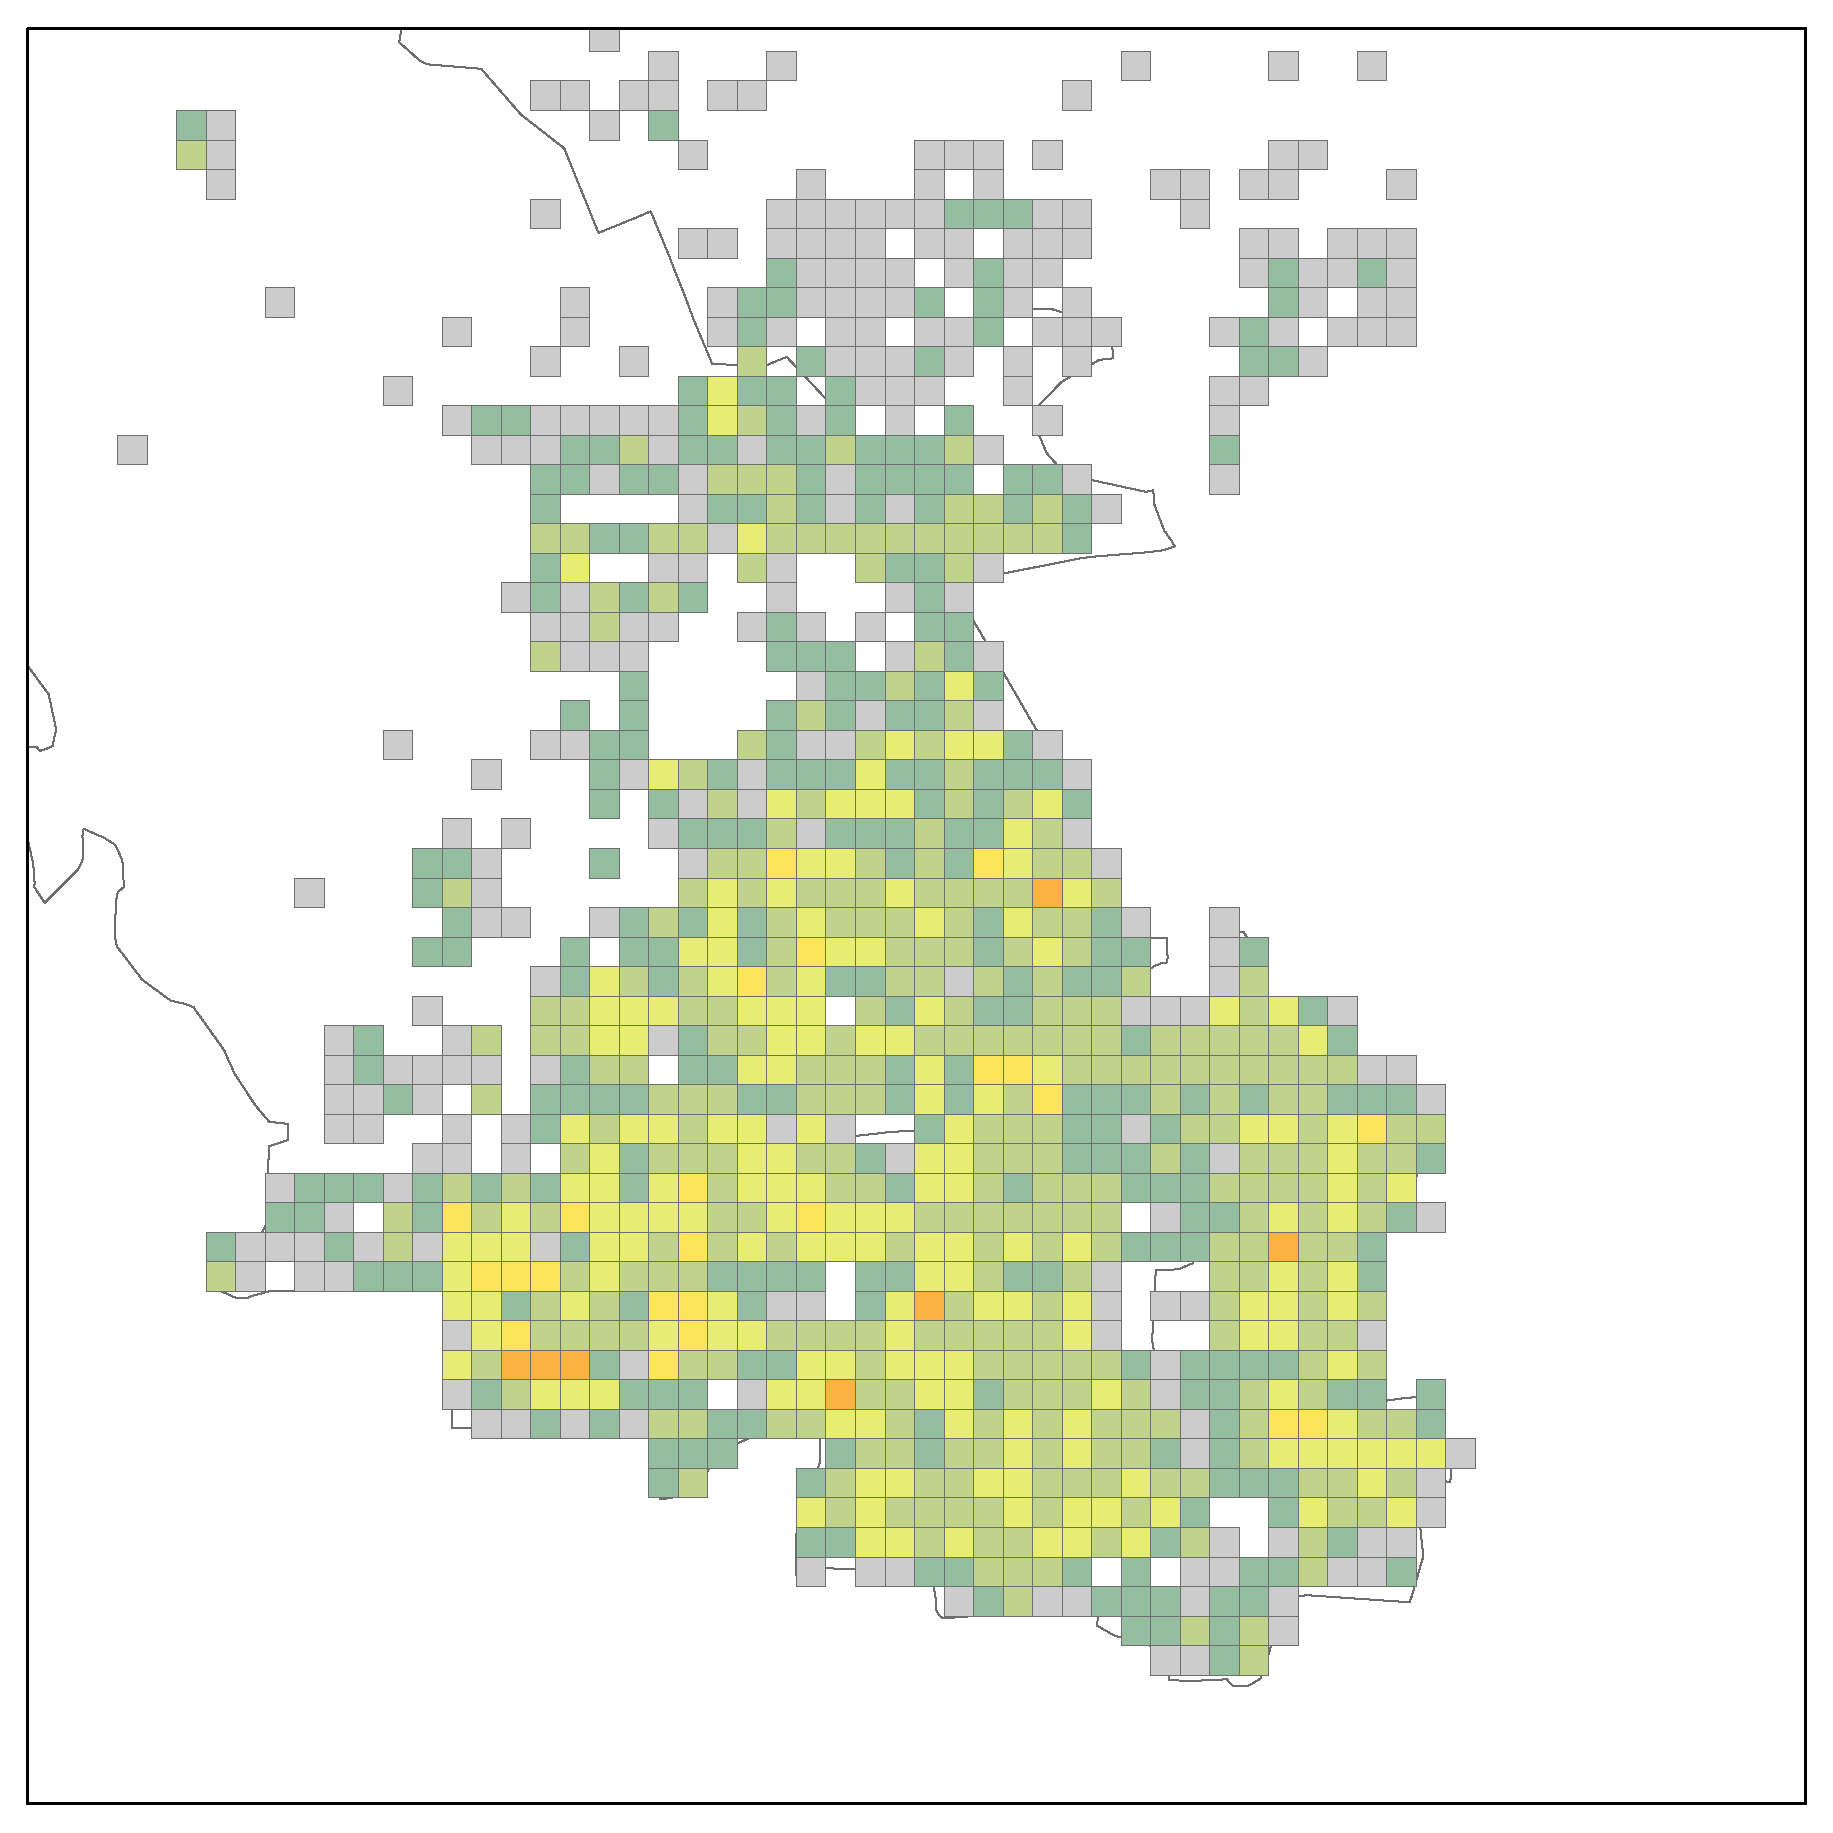
\includegraphics[width=\textwidth]{Figures/Overall_spatial_patterns/FN5_D2020_02_02.eps}
        \caption{02 Feb}
    \end{subfigure}
    
    \vspace{6pt}
    \begin{subfigure}{.23\textwidth}
        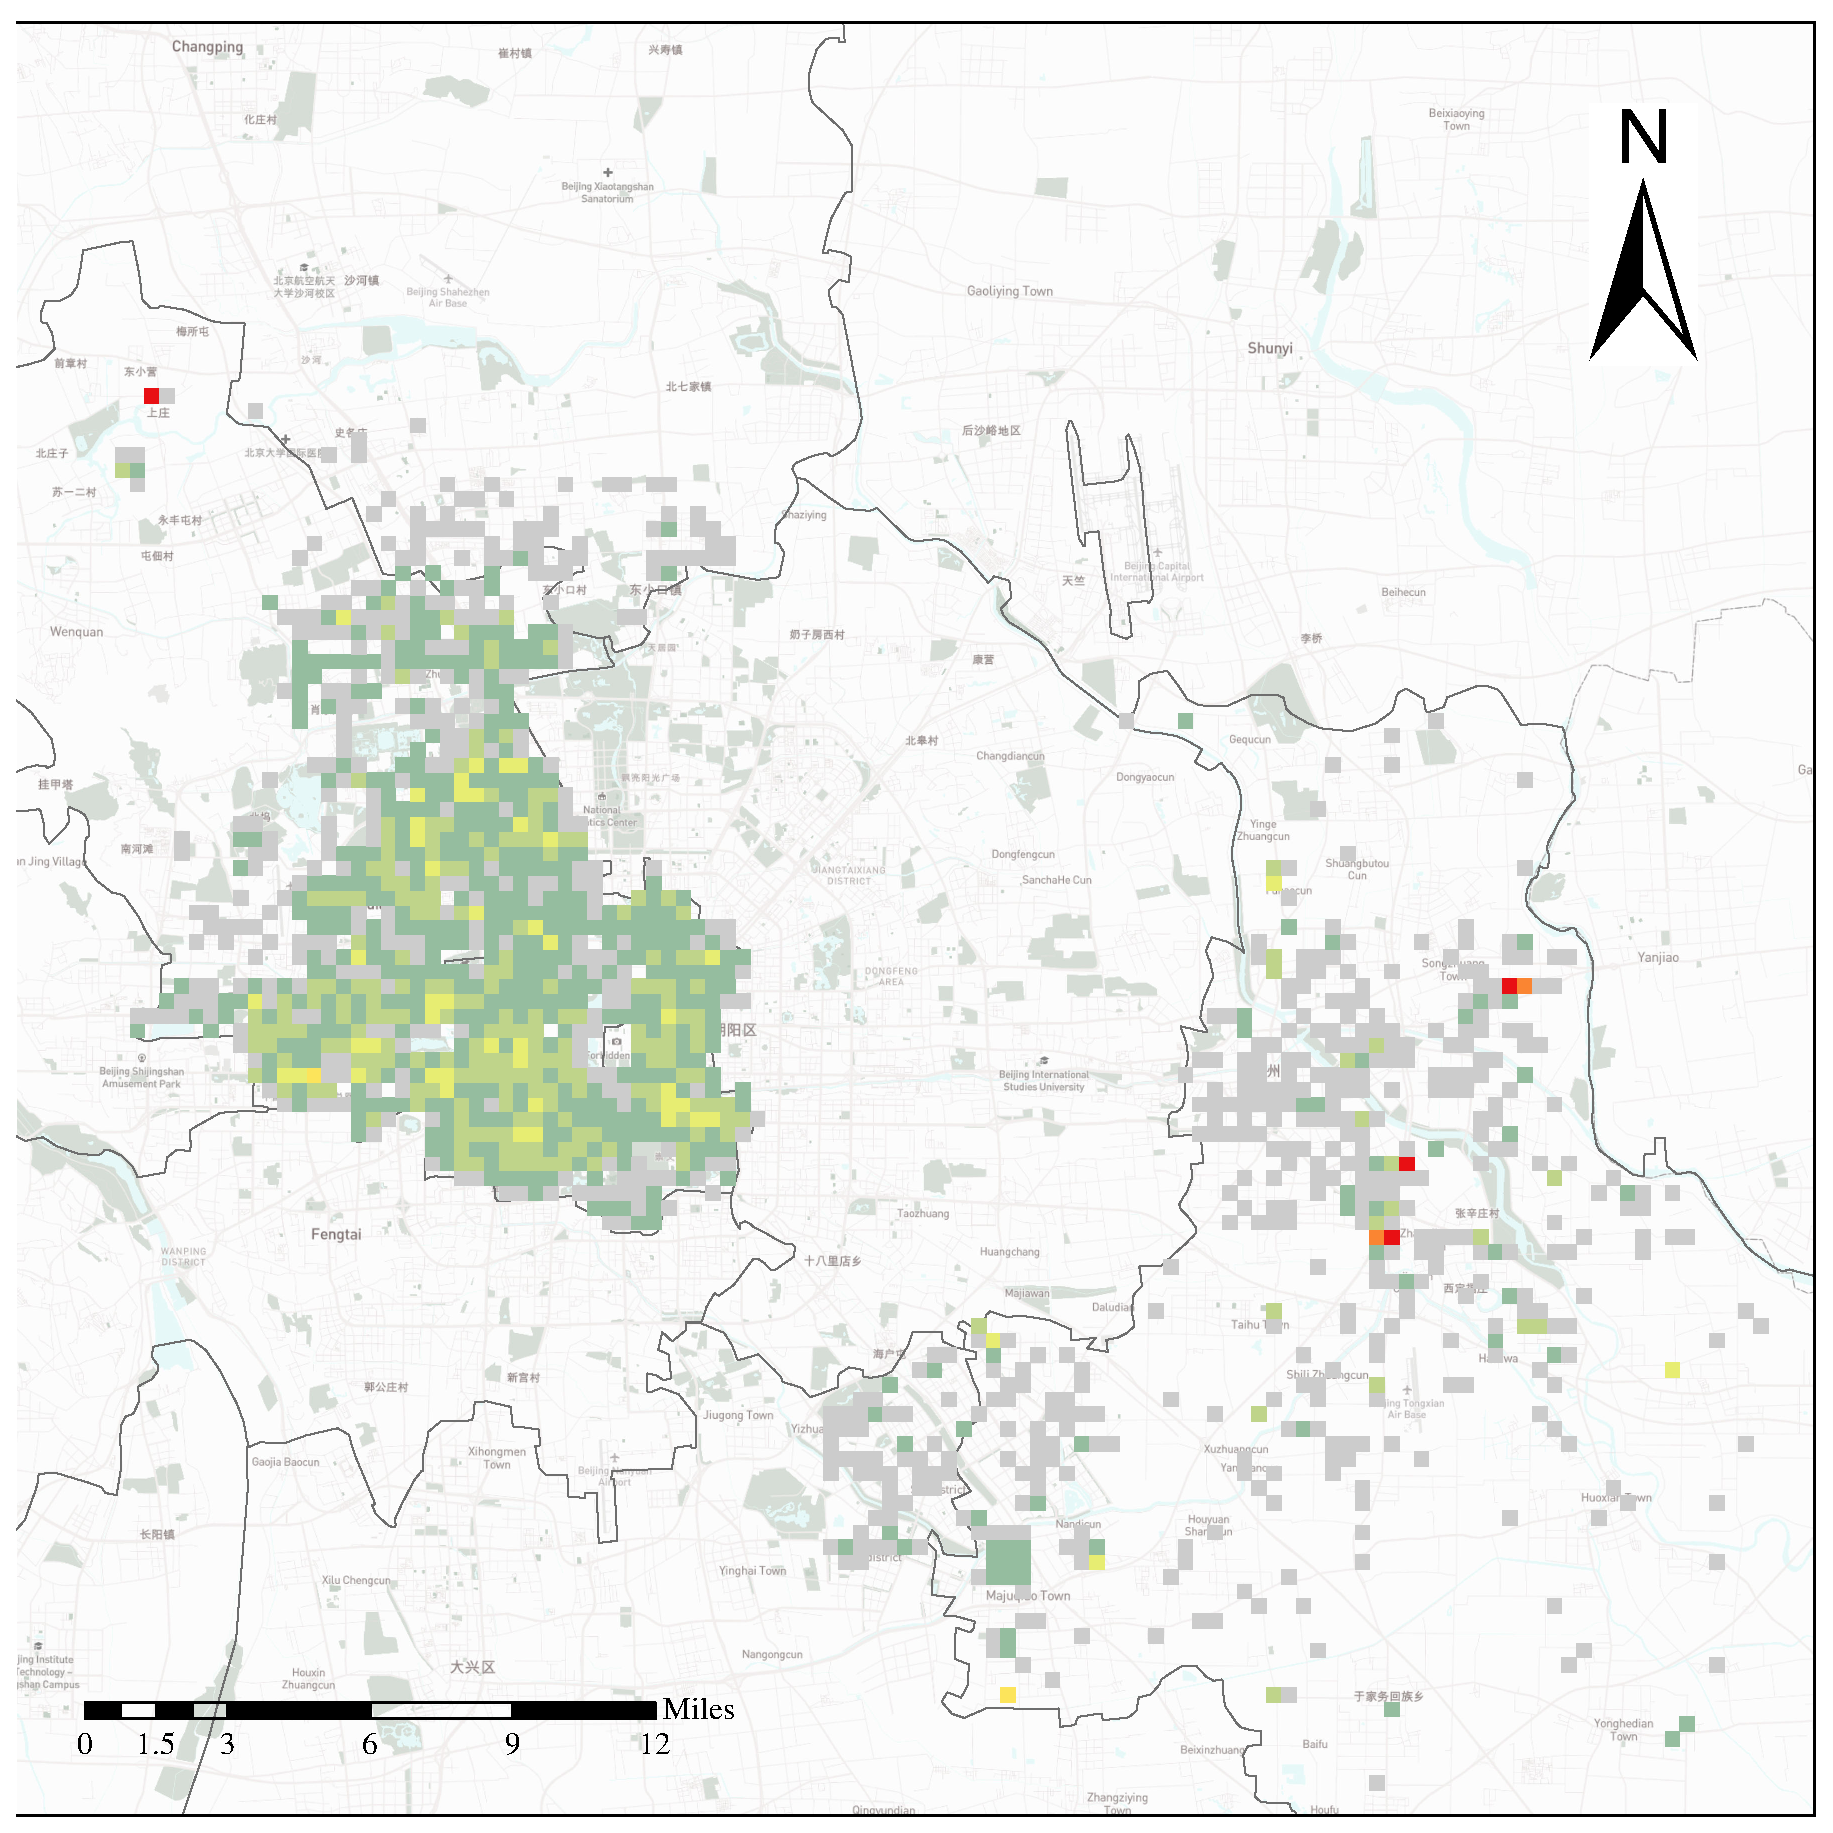
\includegraphics[width=\textwidth]{Figures/Overall_spatial_patterns/FN5_D2020_02_06.eps}
        \caption{06 Feb}
    \end{subfigure}
    \begin{subfigure}{.23\textwidth}
        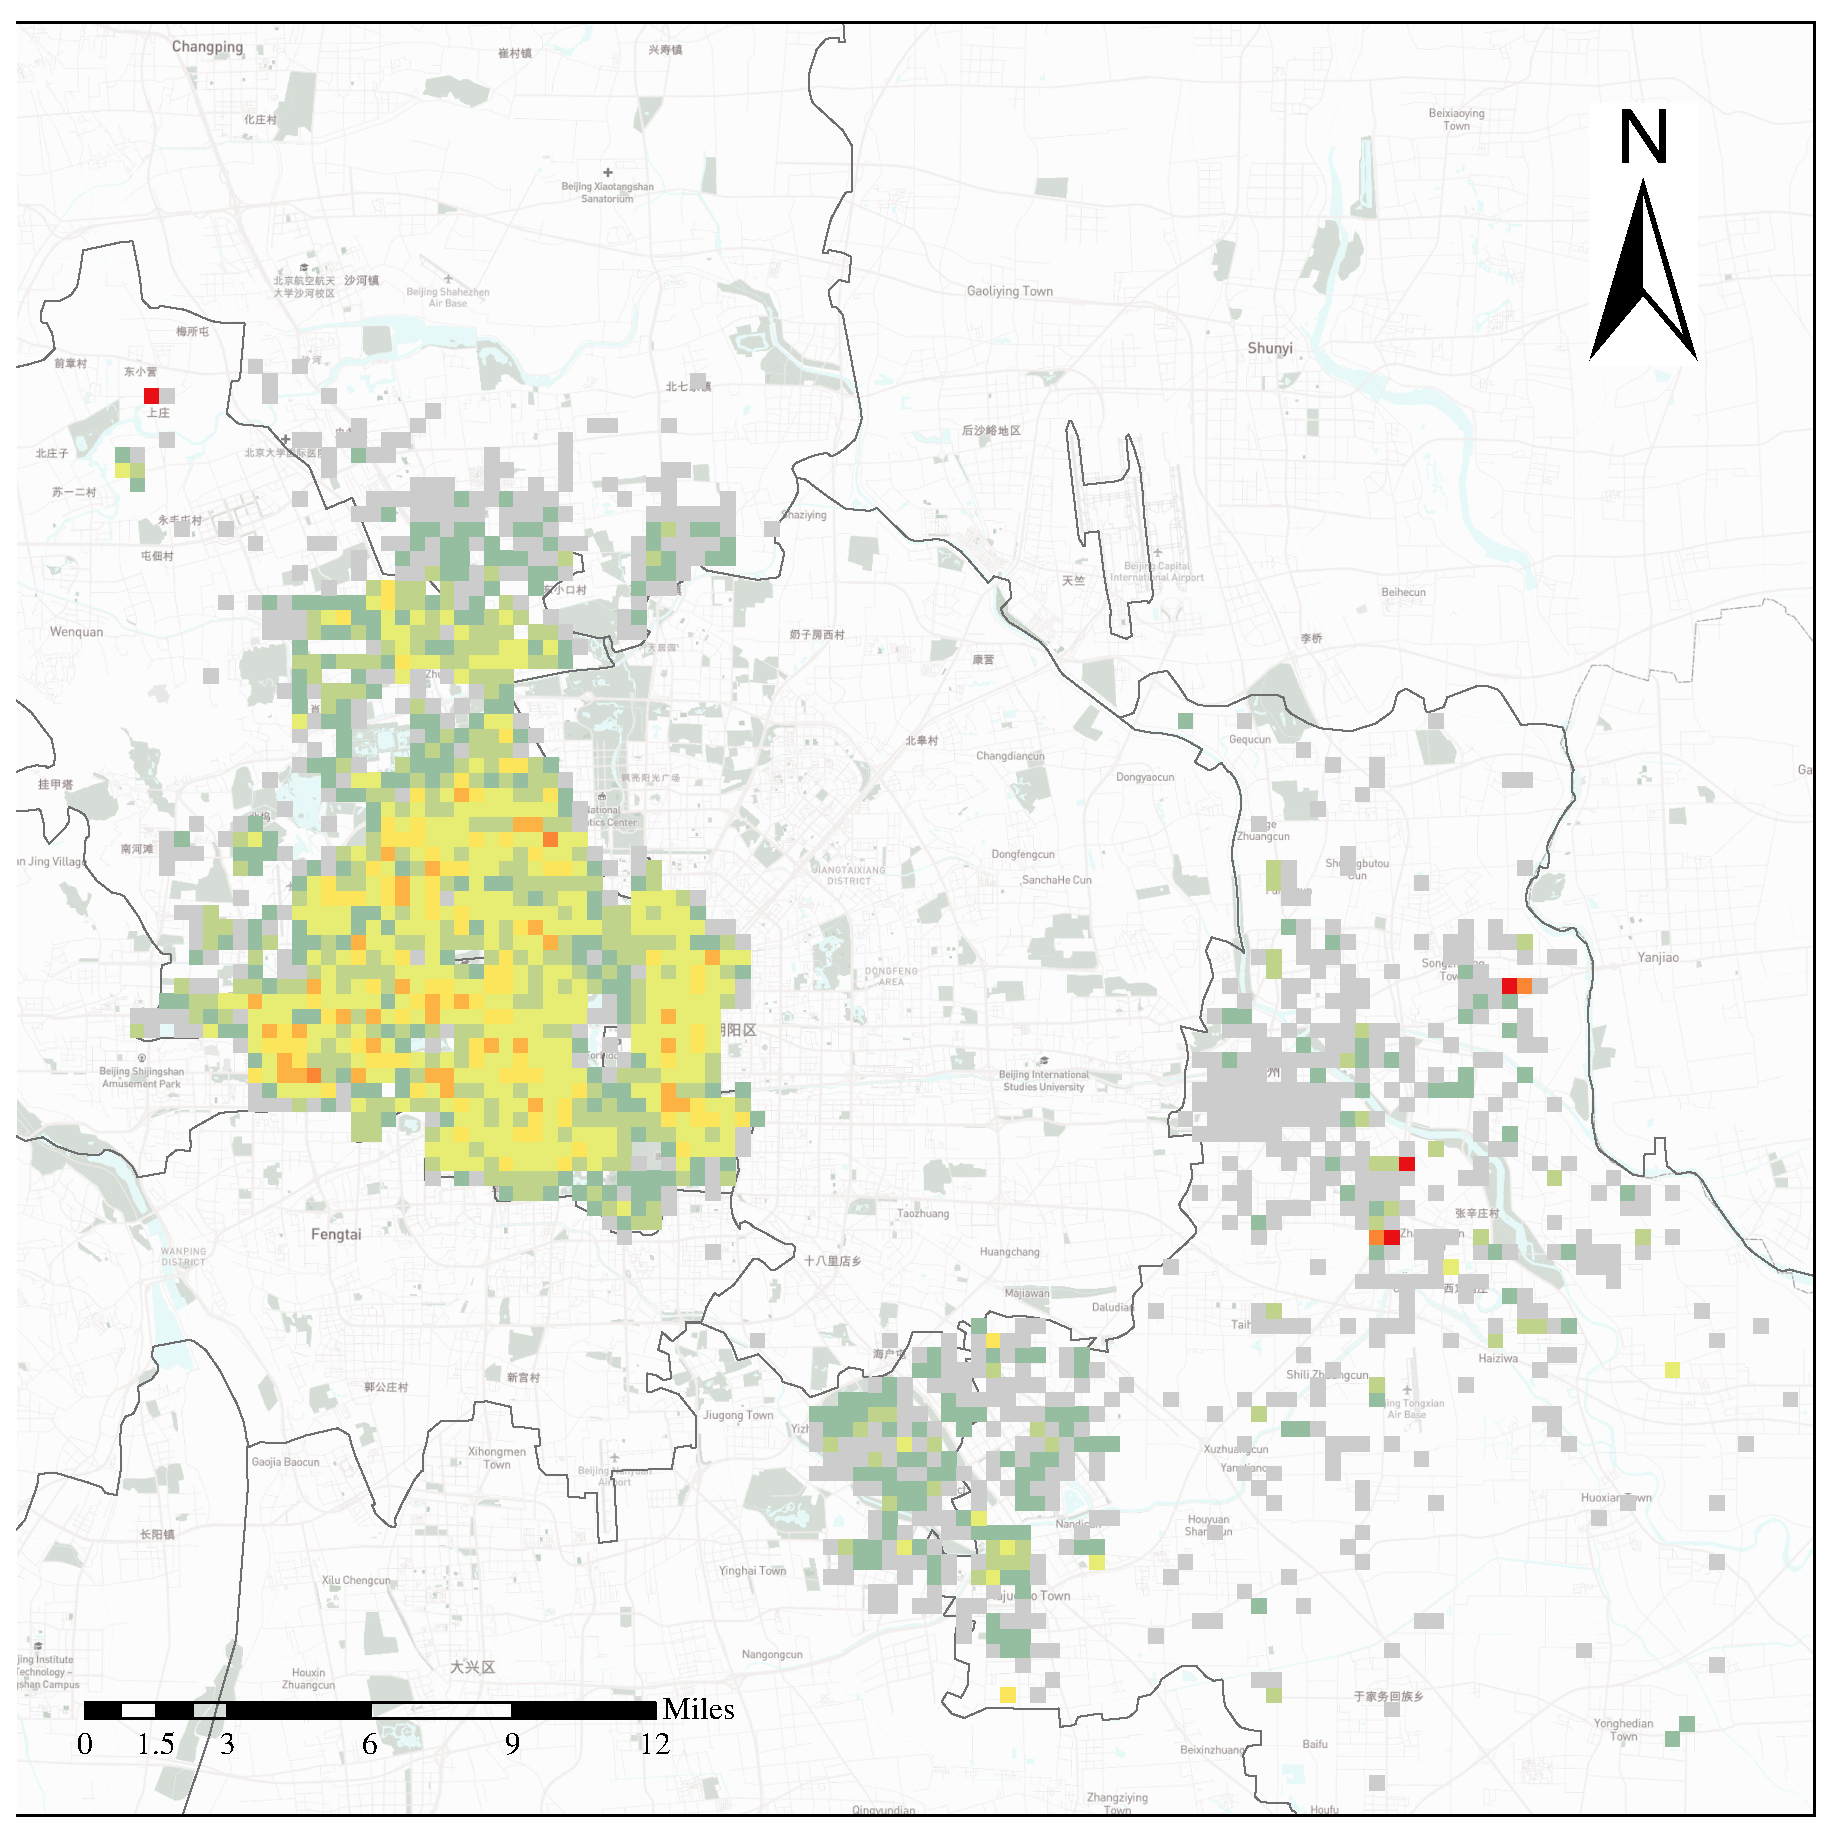
\includegraphics[width=\textwidth]{Figures/Overall_spatial_patterns/FN5_D2020_02_10.eps}
        \caption{10 Feb}\label{fig:pattern_02_10}
    \end{subfigure}
    \begin{subfigure}{.23\textwidth}
        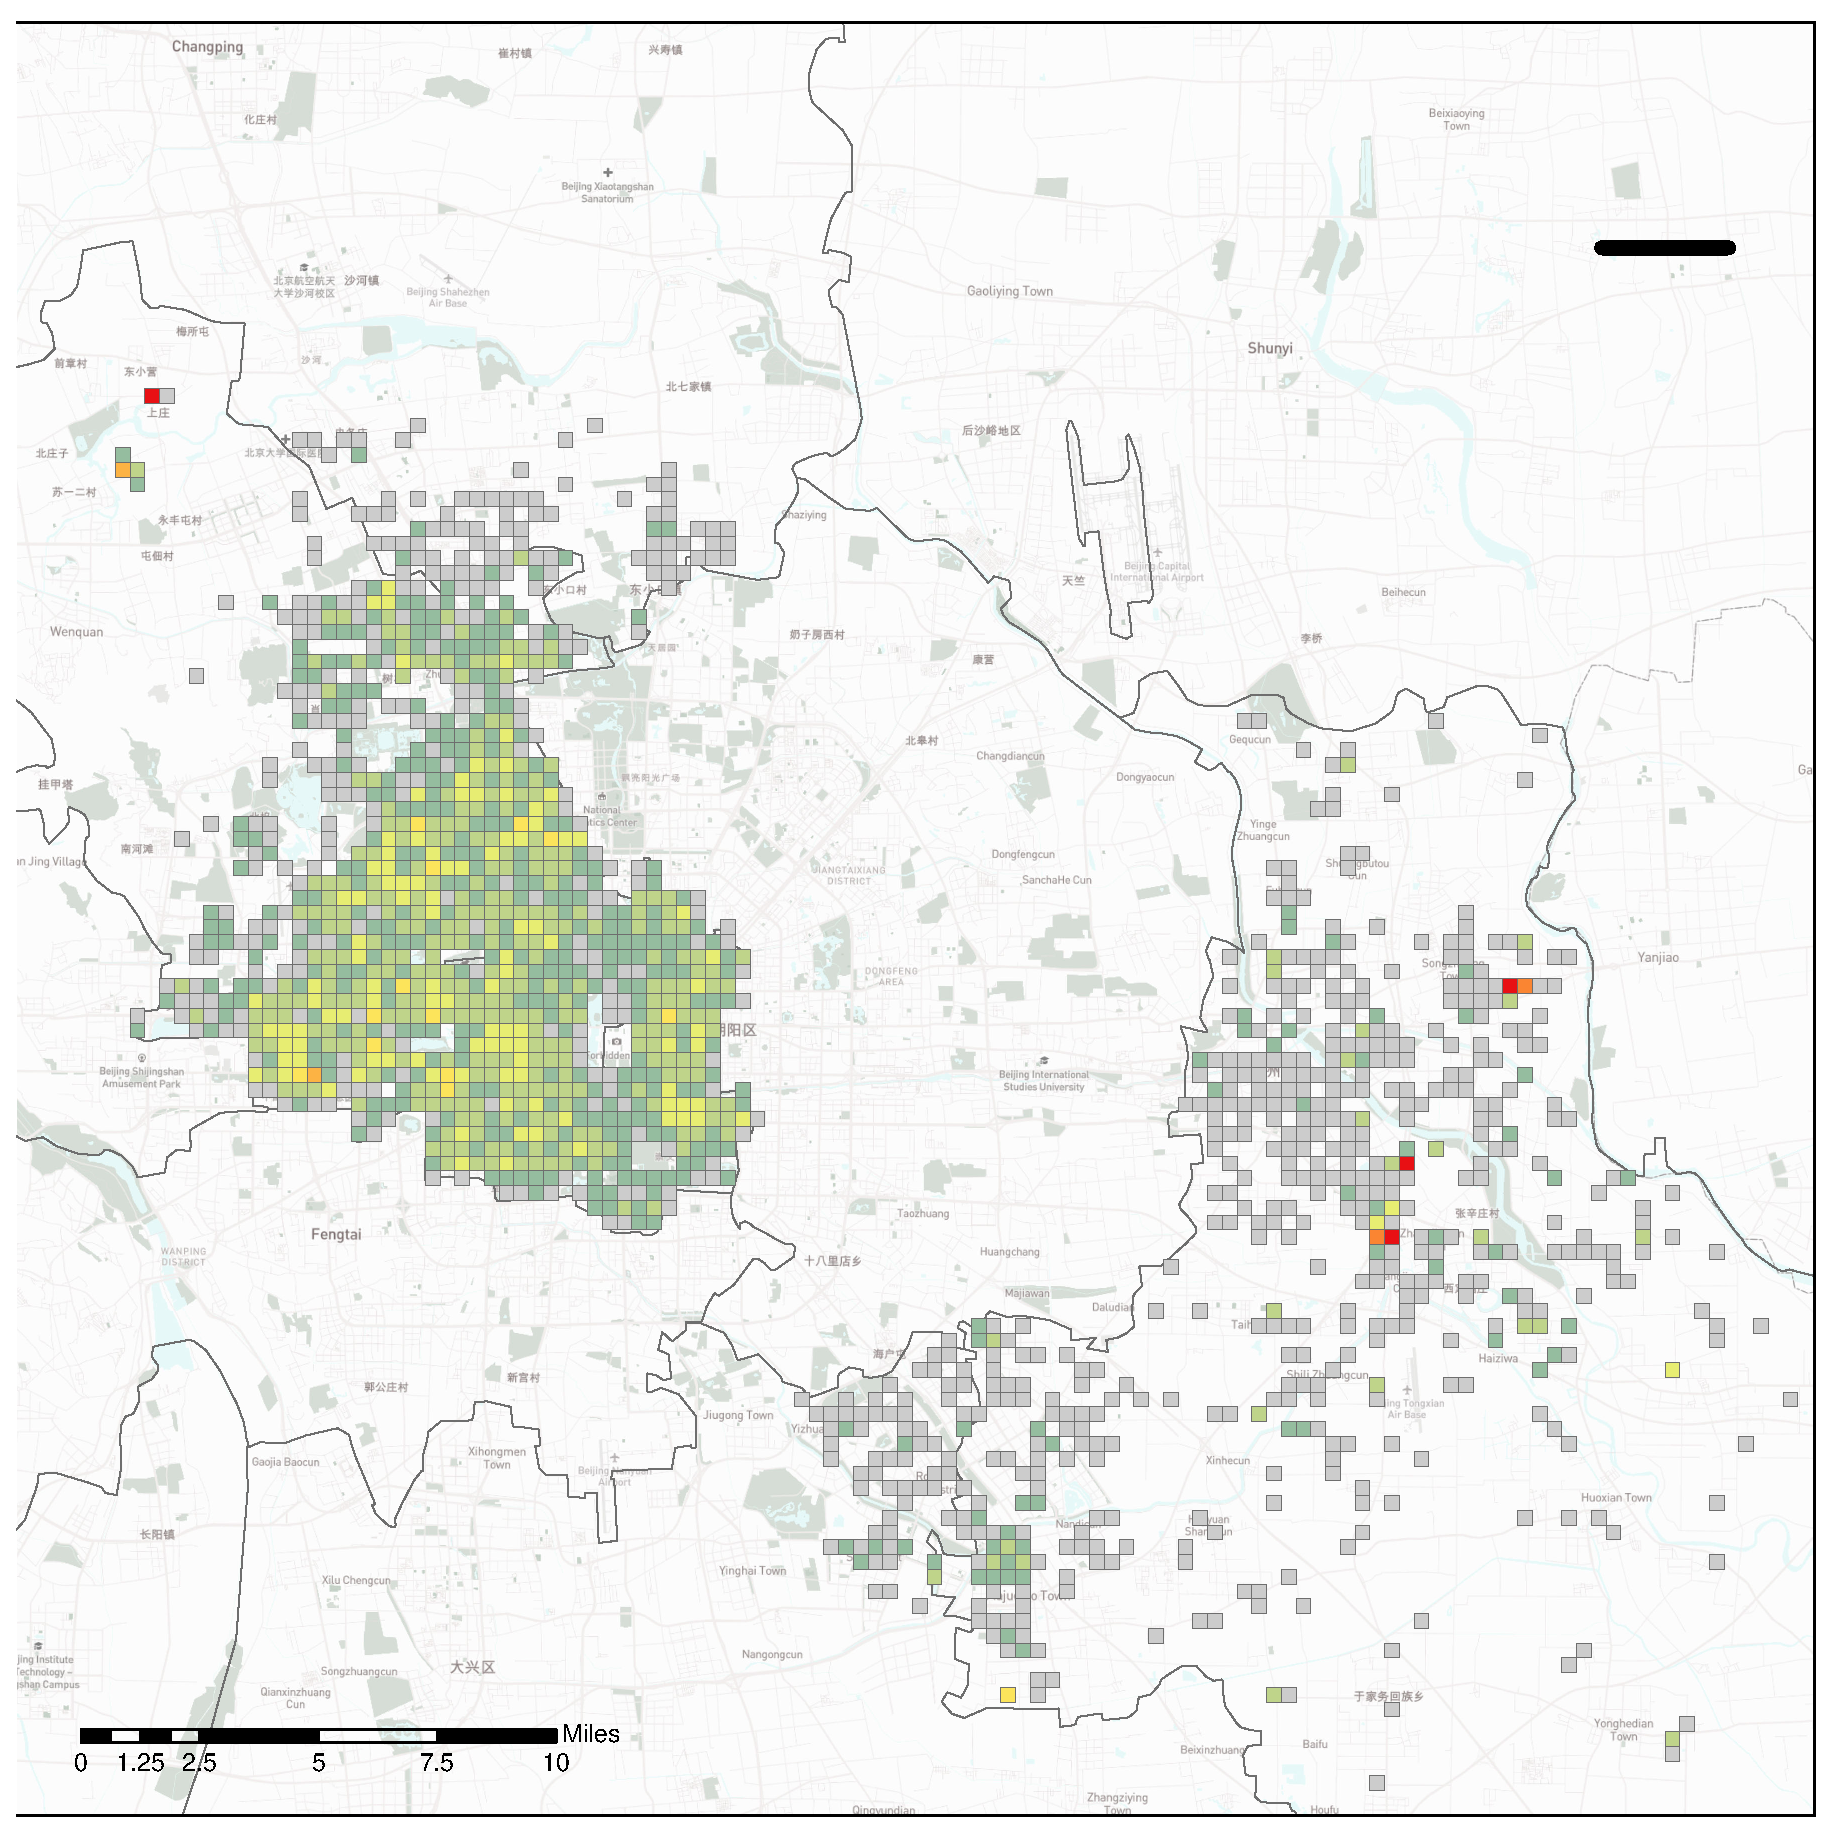
\includegraphics[width=\textwidth]{Figures/Overall_spatial_patterns/FN5_D2020_02_14.eps}
        \caption{14 Feb}
    \end{subfigure}
        \begin{subfigure}{.23\textwidth}
        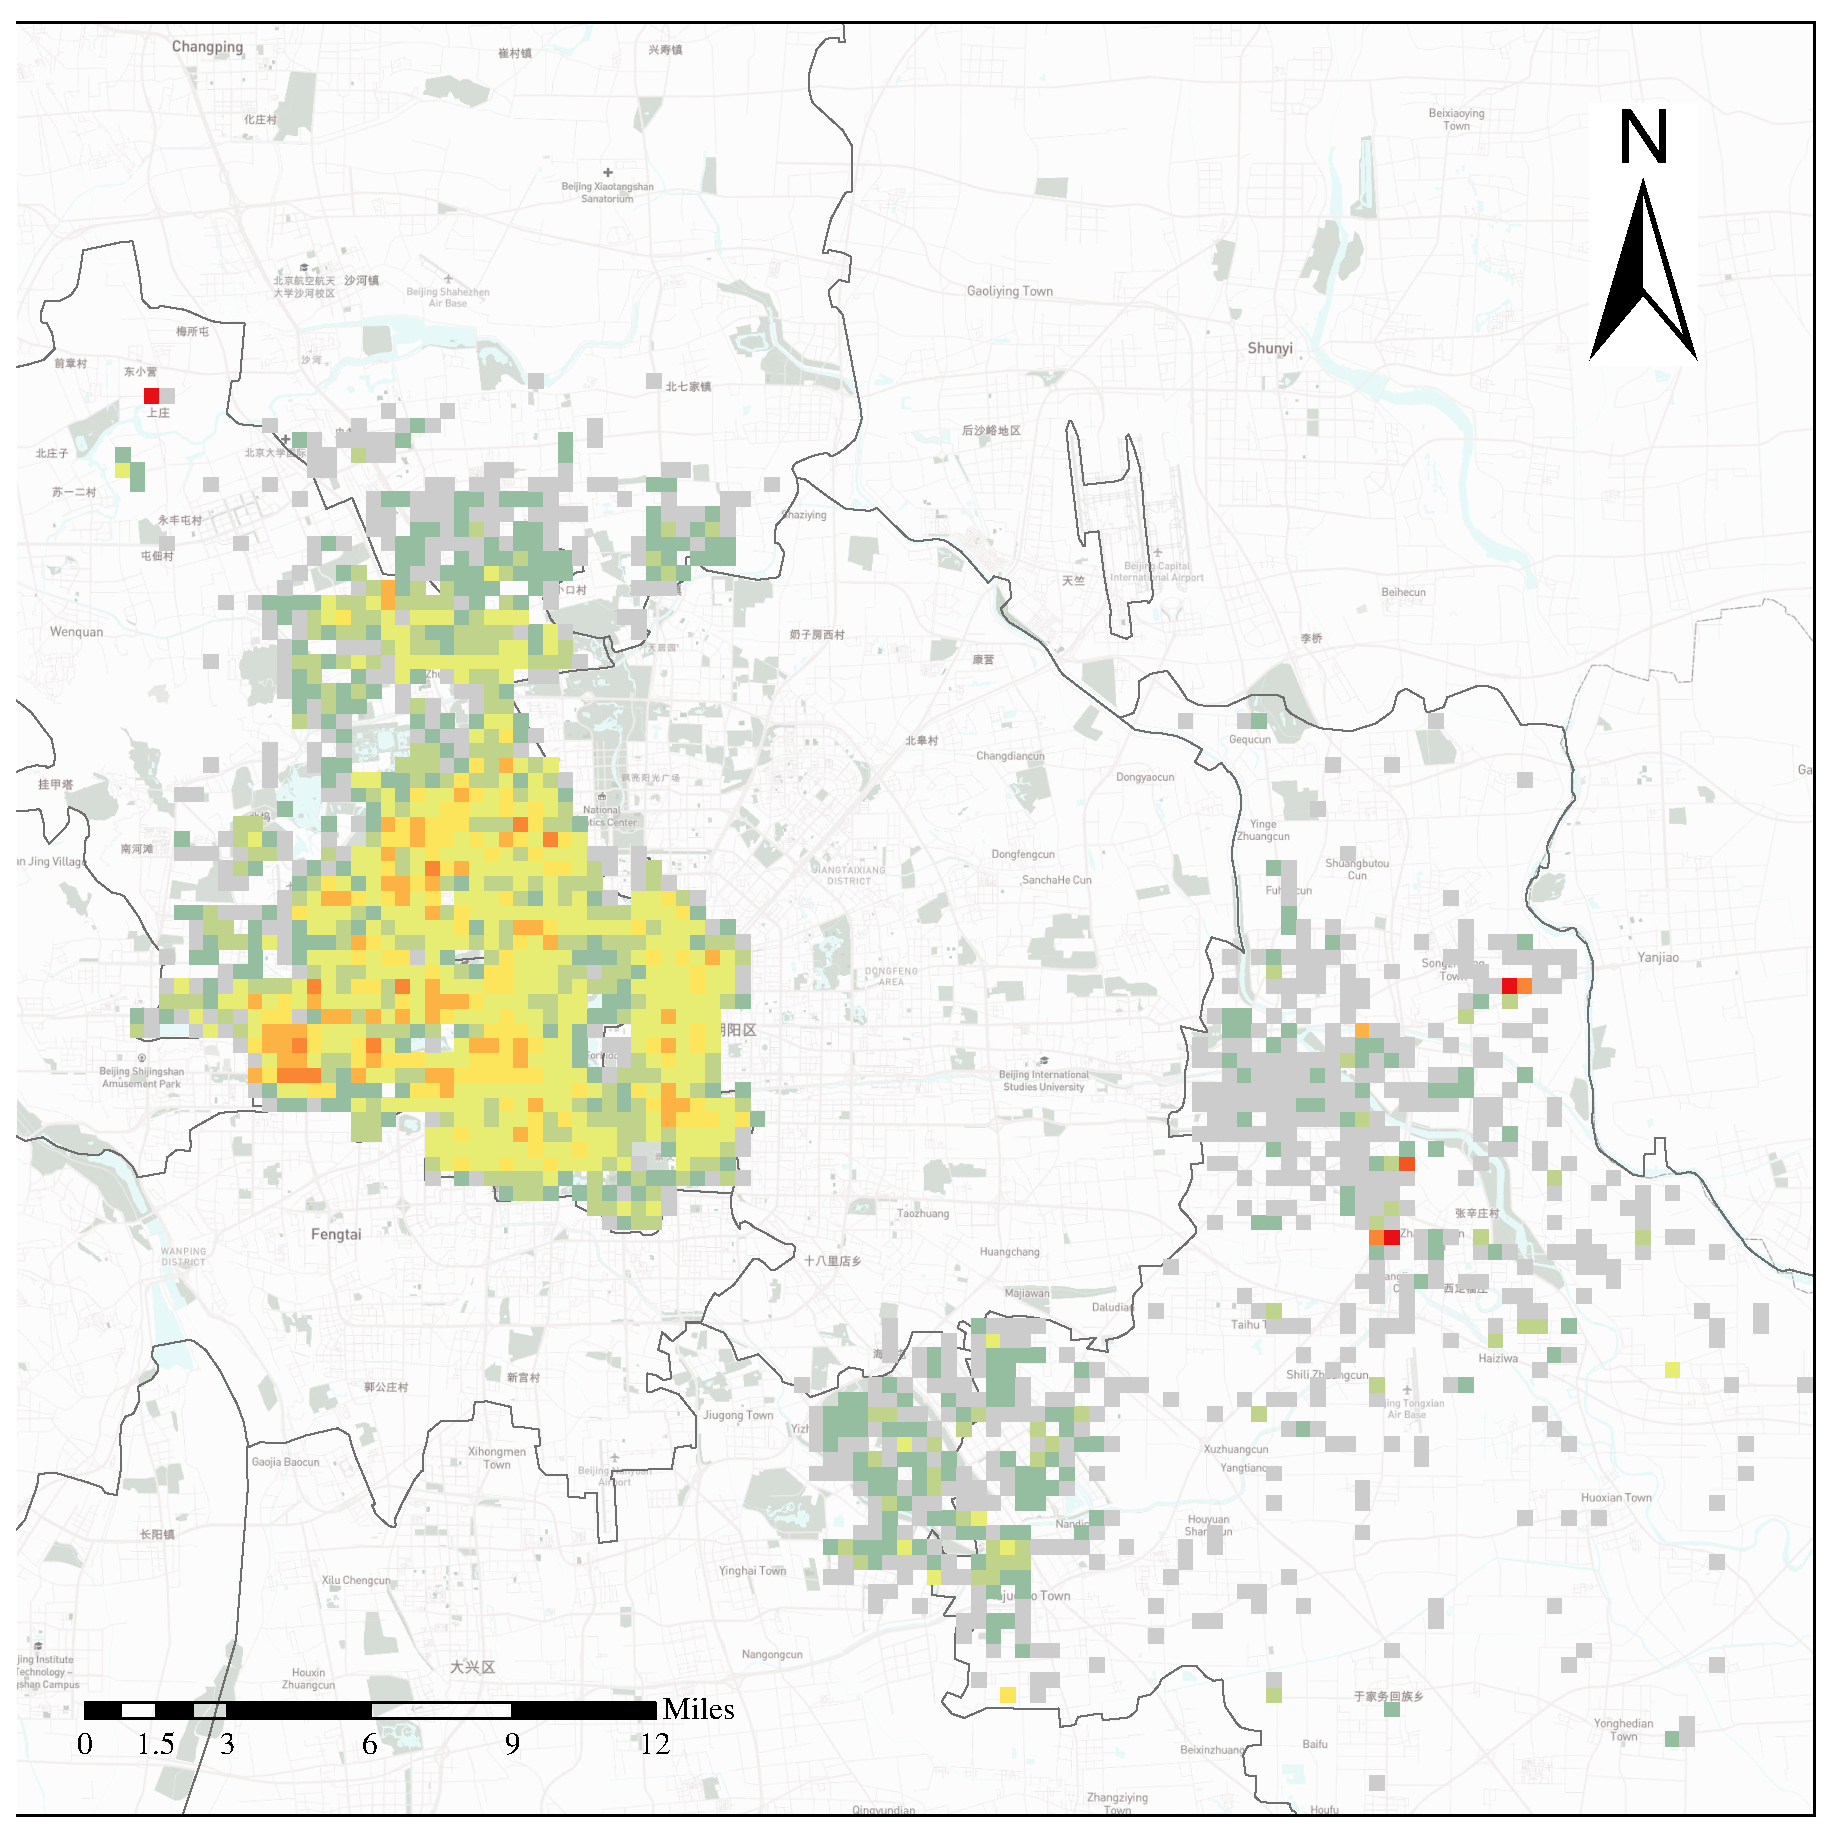
\includegraphics[width=\textwidth]{Figures/Overall_spatial_patterns/FN5_D2020_02_18.eps}
        \caption{18 Feb}
    \end{subfigure}
    
    \vspace{6pt}
    \begin{subfigure}{.23\textwidth}
        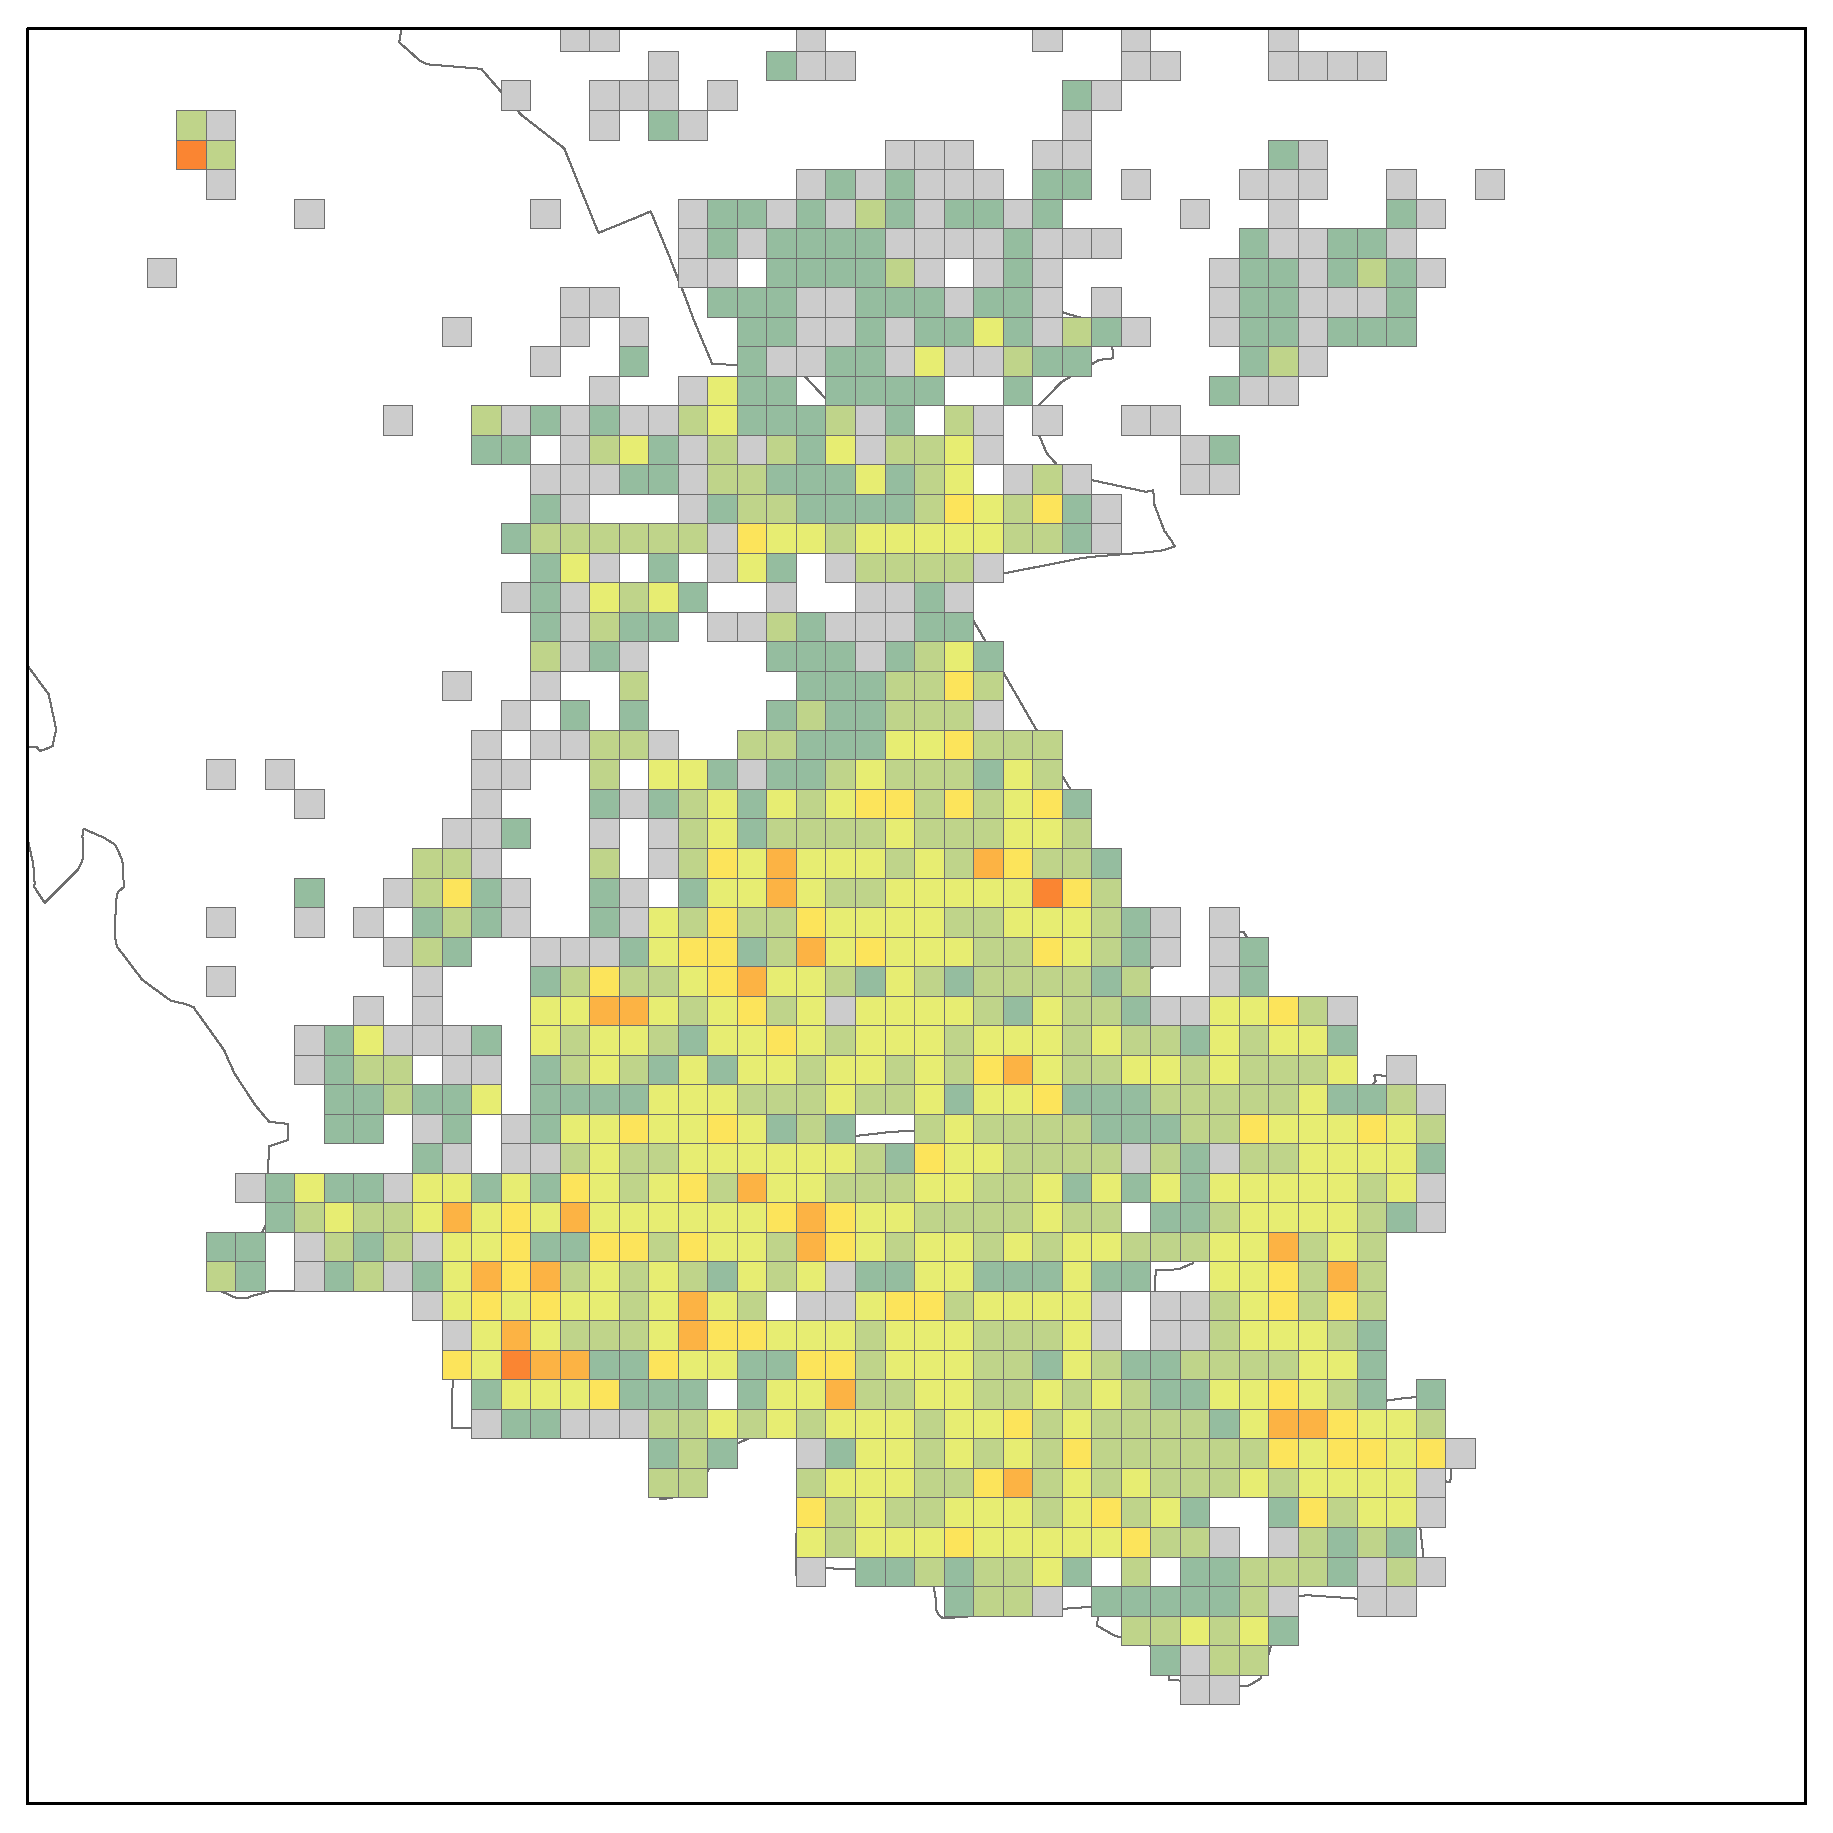
\includegraphics[width=\textwidth]{Figures/Overall_spatial_patterns/FN5_D2020_02_22.eps}
        \caption{24 Feb}
    \end{subfigure}
    \begin{subfigure}{.23\textwidth}
        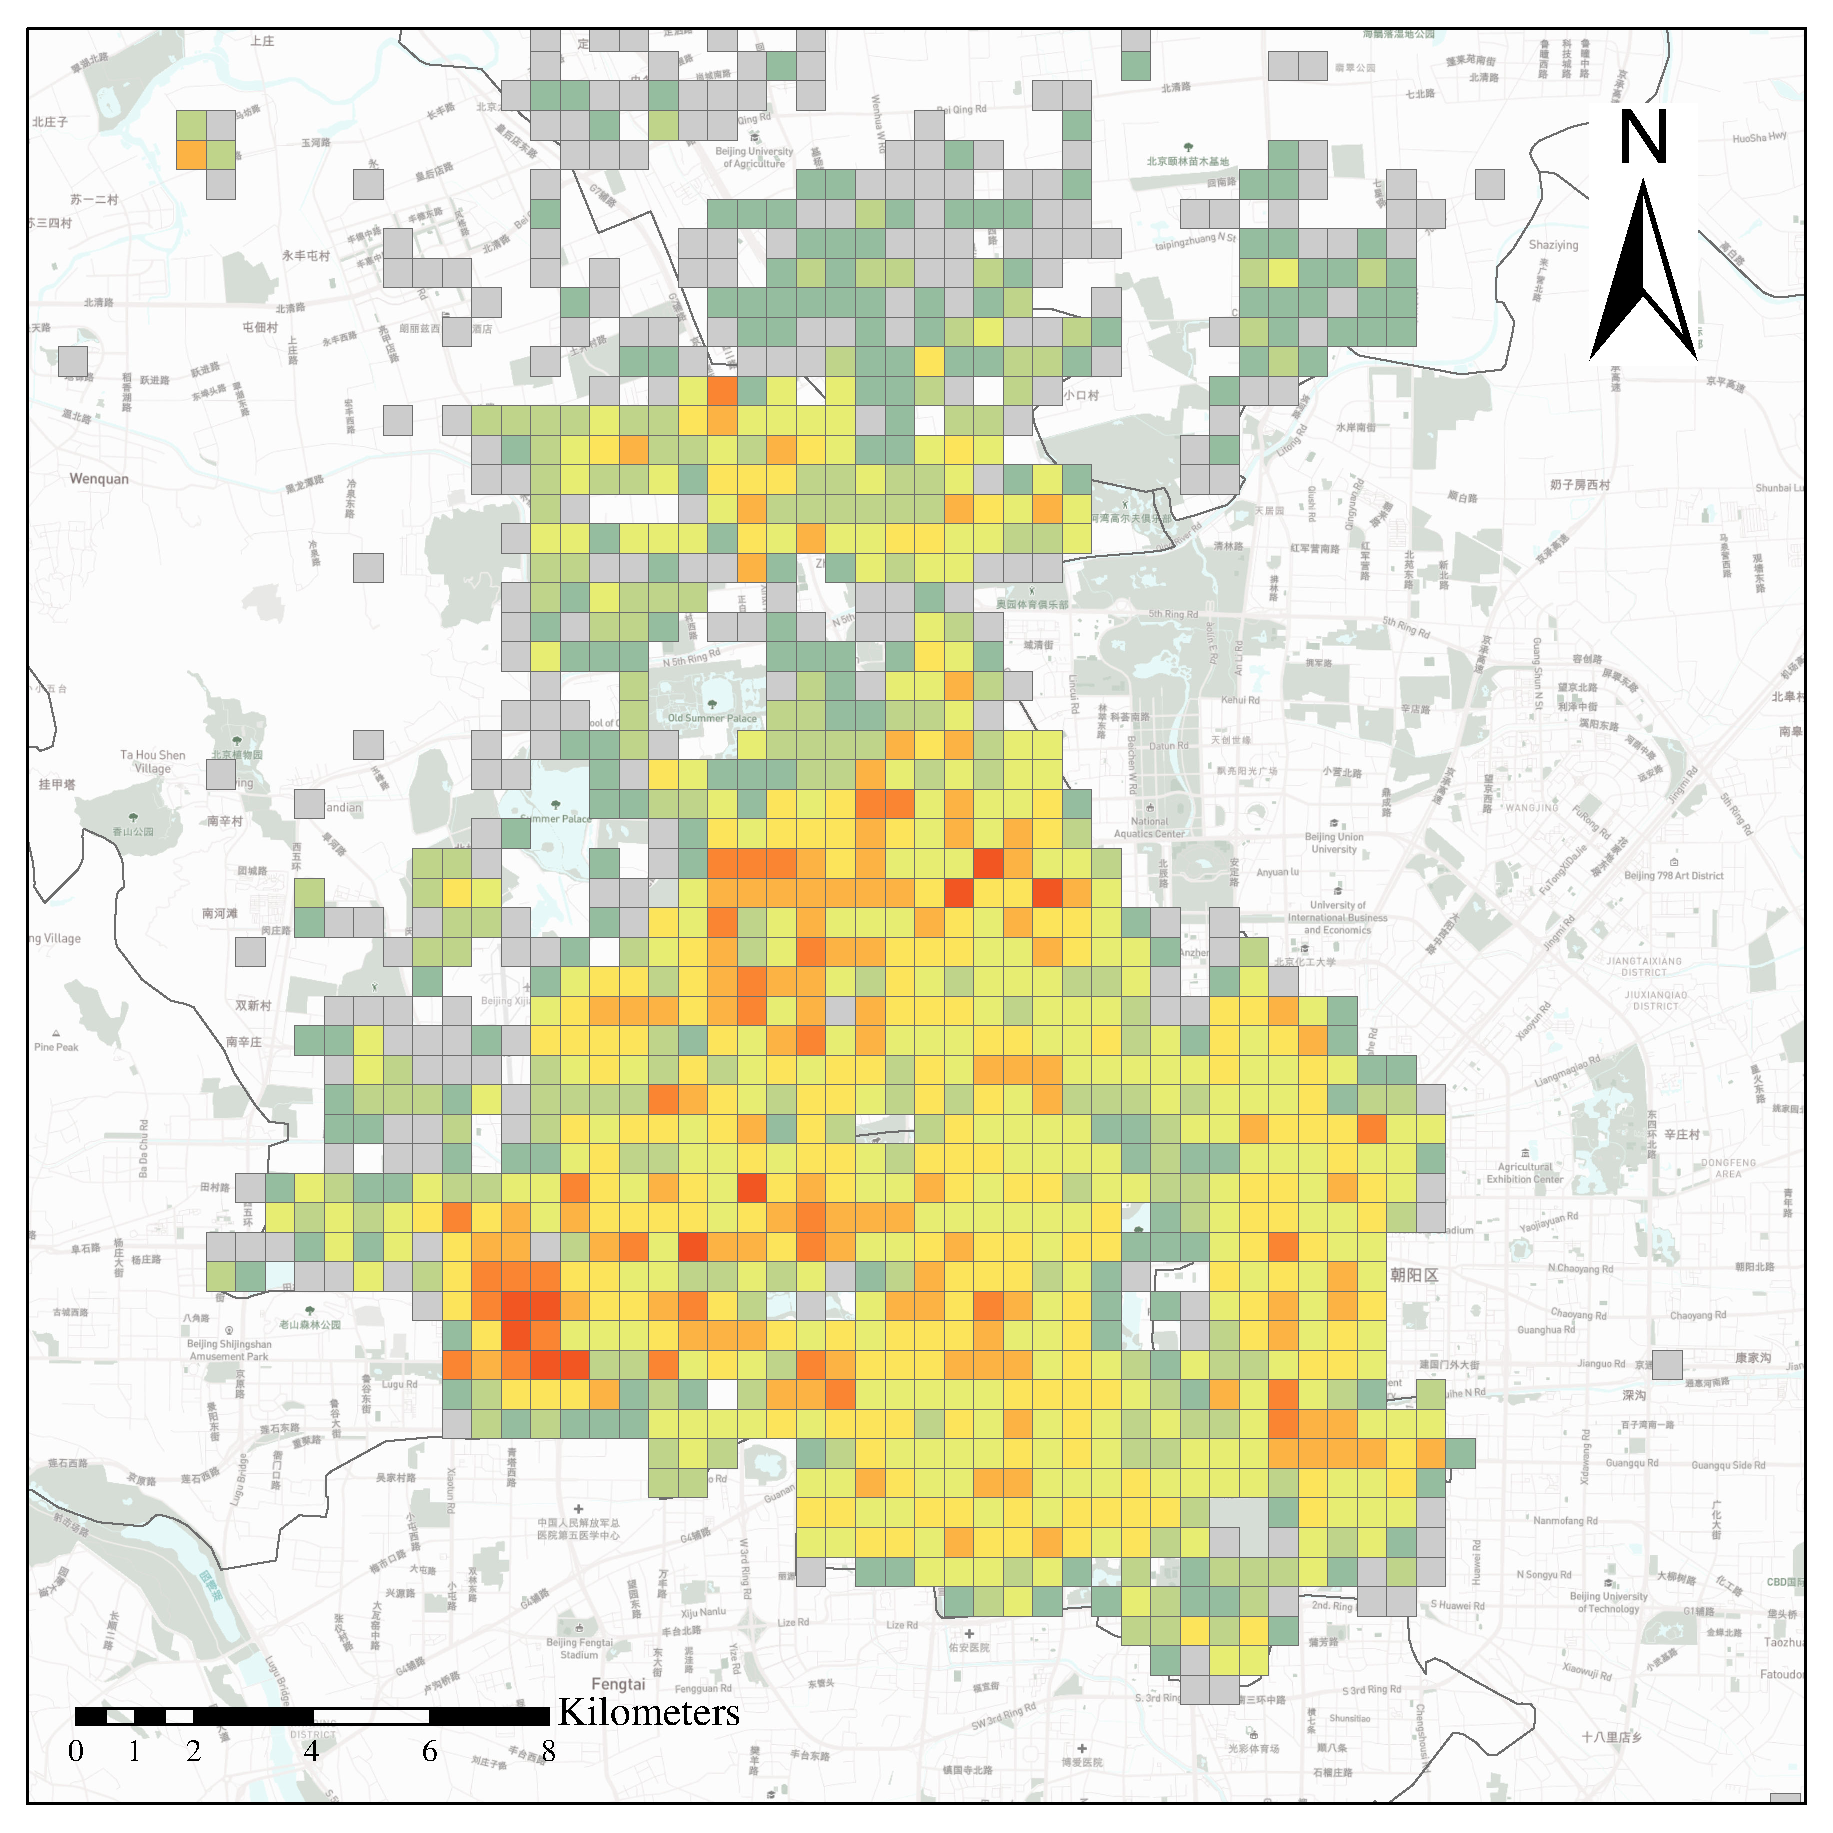
\includegraphics[width=\textwidth]{Figures/Overall_spatial_patterns/FN5_D2020_02_26.eps}
        \caption{26 Feb}
    \end{subfigure}
    \begin{subfigure}{.23\textwidth}
        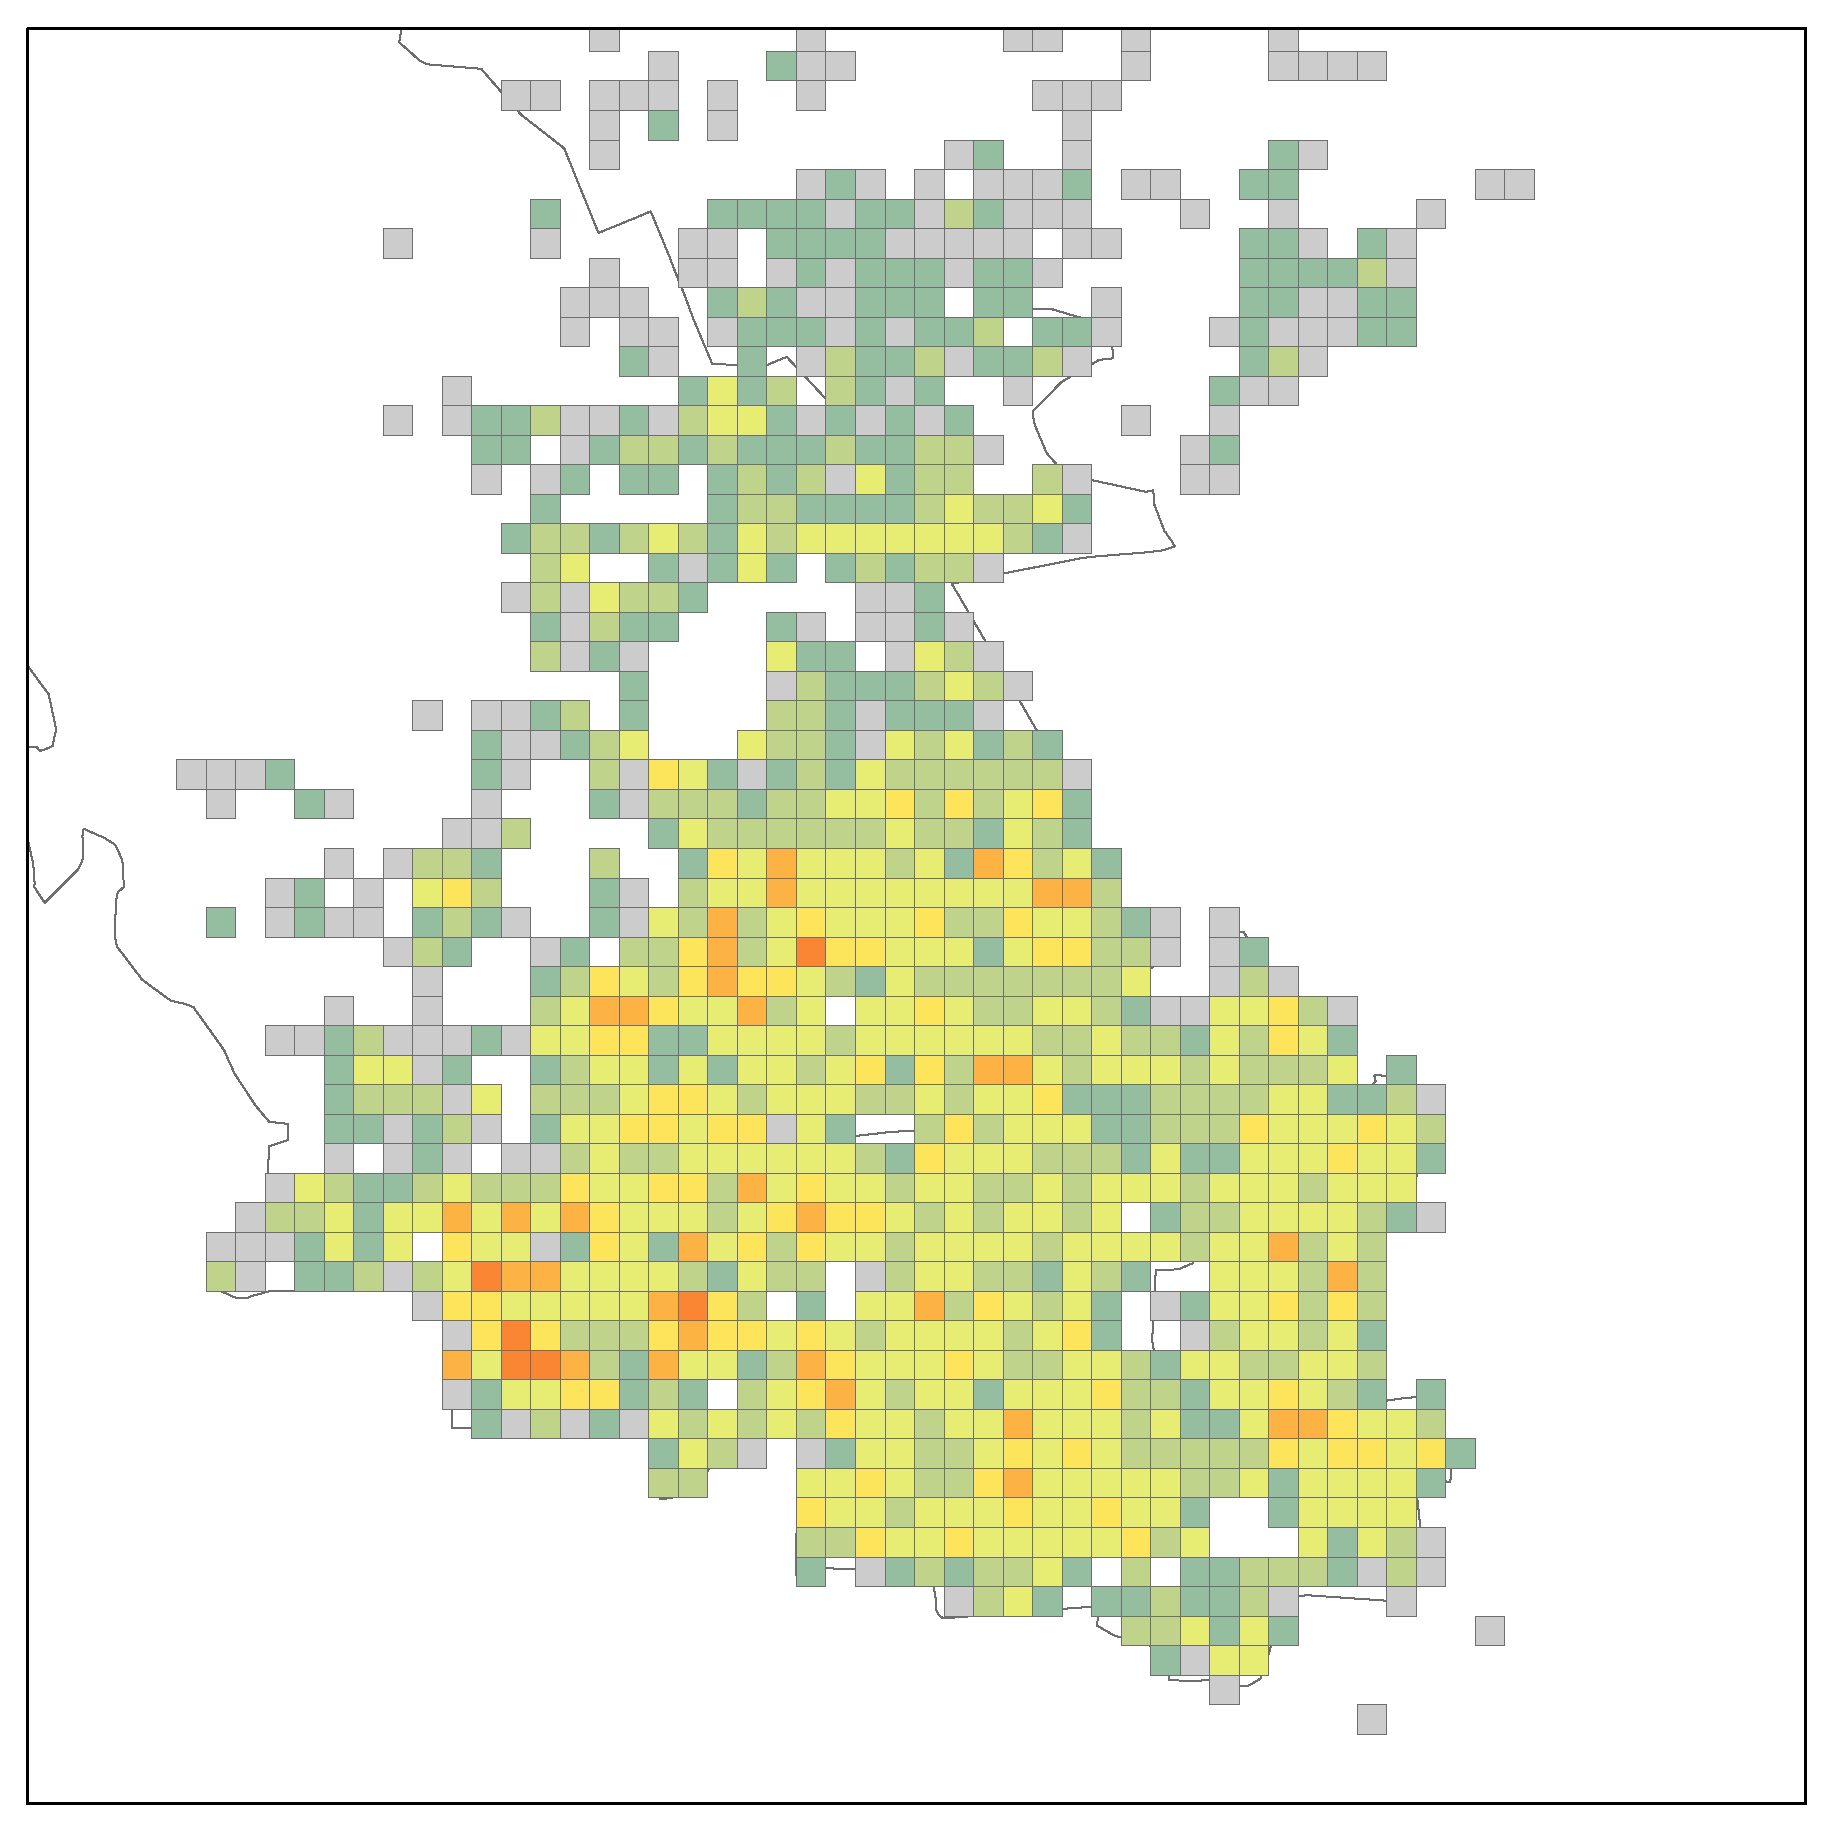
\includegraphics[width=\textwidth]{Figures/Overall_spatial_patterns/FN5_D2020_03_01.eps}
        \caption{01 Mar}\label{fig:pattern_03_01}
    \end{subfigure}
    \begin{subfigure}{.13\textwidth}
        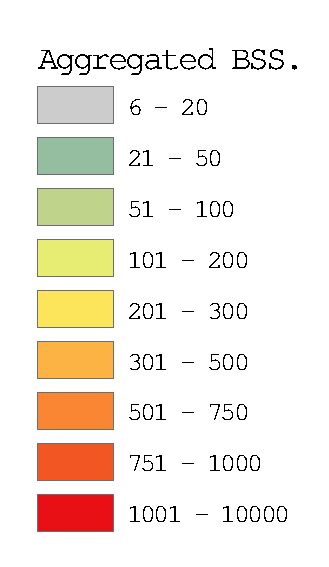
\includegraphics[width=\textwidth]{Figures/Overall_spatial_patterns/legend5.eps}
        \caption{Legend}
    \end{subfigure}
    \caption{Spatial patterns of cycling activities from 21 Jan to 01 March 2020}
    \label{fig:full_spatial_pattern_2020}
\end{figure}

Figure \ref{fig:full_spatial_pattern_2020} shows the spatial patterns of BSS activities from 21 Jan to 02 Mar by 4-day intervals, which is consistent with the changes detected in Figure \ref{fig:hour_comparison_8}. % and \ref{fig:hour_comparison_18}.
The daily share bike records are aggregated within 500-meter grids, and rendered with a color ramp from grey to green to red (as is in Legend).

Before 21 Jan, 2020, share bike activities were widely distributed throughout the city limits, with a significant concentration in downtown area, which is orange or even red in color, corresponding to high-intensity activities (up to 500-1000 records/hour).
These patterns could be regarded as a comprehensive reflection of the activities of the individuals in these regions, and used as a reference to compare with that during COVID-19 pandemic.

After the COVID-19 outbreak, there is a dramatic drop in mobility since 25 Jan, which was also the begining of the Chinese New Year holidays.
High-intensity activities could hardly be recognized in the subfigures between 25 Jan to 02 Feb. 
These subfigures are dominated by green and light green corresponding to low-intensity activities (<100 records/hour), indicating that individuals have demands to go out during this period, but unnecessary going-out has been significantly reduced by the combined effects of holidays and the epidemic.
Status continued until 09 Feb, when the spread of COVID-19 was slowered down by imposing control measures including social distancing and home quarantine, and productive and social activities were allowed to restart partially.

Figure \ref{fig:pattern_02_10}-\ref{fig:pattern_03_01} during 10 Feb to 01 Mar, 2020, show a gradual increase in the mobility of the SBs, but only restored around $30\%$ of the pre-epidemic levels.
It is worth noticing that only slight differences could be observed between weekdays and weekends before 17 Feb and the weekday-weekend oscillation returned afterwards.

There is a higher demand for SBs on workdays in the downtown area as before.
However, the high-intensity areas shrinked on weekends, implying that residents were more inclined to reduce the risk of increased exposure by going outside under the threat of COVID-19. 

Inferred from the spatiotemporal characteristics above, the outbreak was divided into 3 phases to better reflect the dynamics of the COVID-19 epidemic.

\textbf{Phase a}: dates before 21 Jan, 2020, are considered as the first period, when no strong COVID-19–specific interventions were imposed.

\textbf{Phase b}: dates between 22 Jan and 17 Feb, include Chinese New Year holiday 2020. During this period, traffic suspension and home quarantine were implemented for pandemics prevention purposes.

\textbf{Phase c}: is after 10 Feb, when productive and social activities restarted partially since the pandemics was migitated and under effective control.

% In the following sections, we will focus on …… and investigate ……

\section{Discussions}
\subsection{Comparison between 2019 and 2020}% in the same period}

Both Chinese New Year holiday shutdowns and pandemic resulted in the aforementioned mobility decrease.
Therefore, comparison was conducted with data from the same period in 2019, thus removing the impact of the Chinese New Year holiday and evaluating the specific influence of the pandemic.  
The average values of aggregated daily SBs records from each pandemic phase were reported.

\begin{figure}[ht]
    \centering
    \begin{subfigure}{.3\textwidth}
        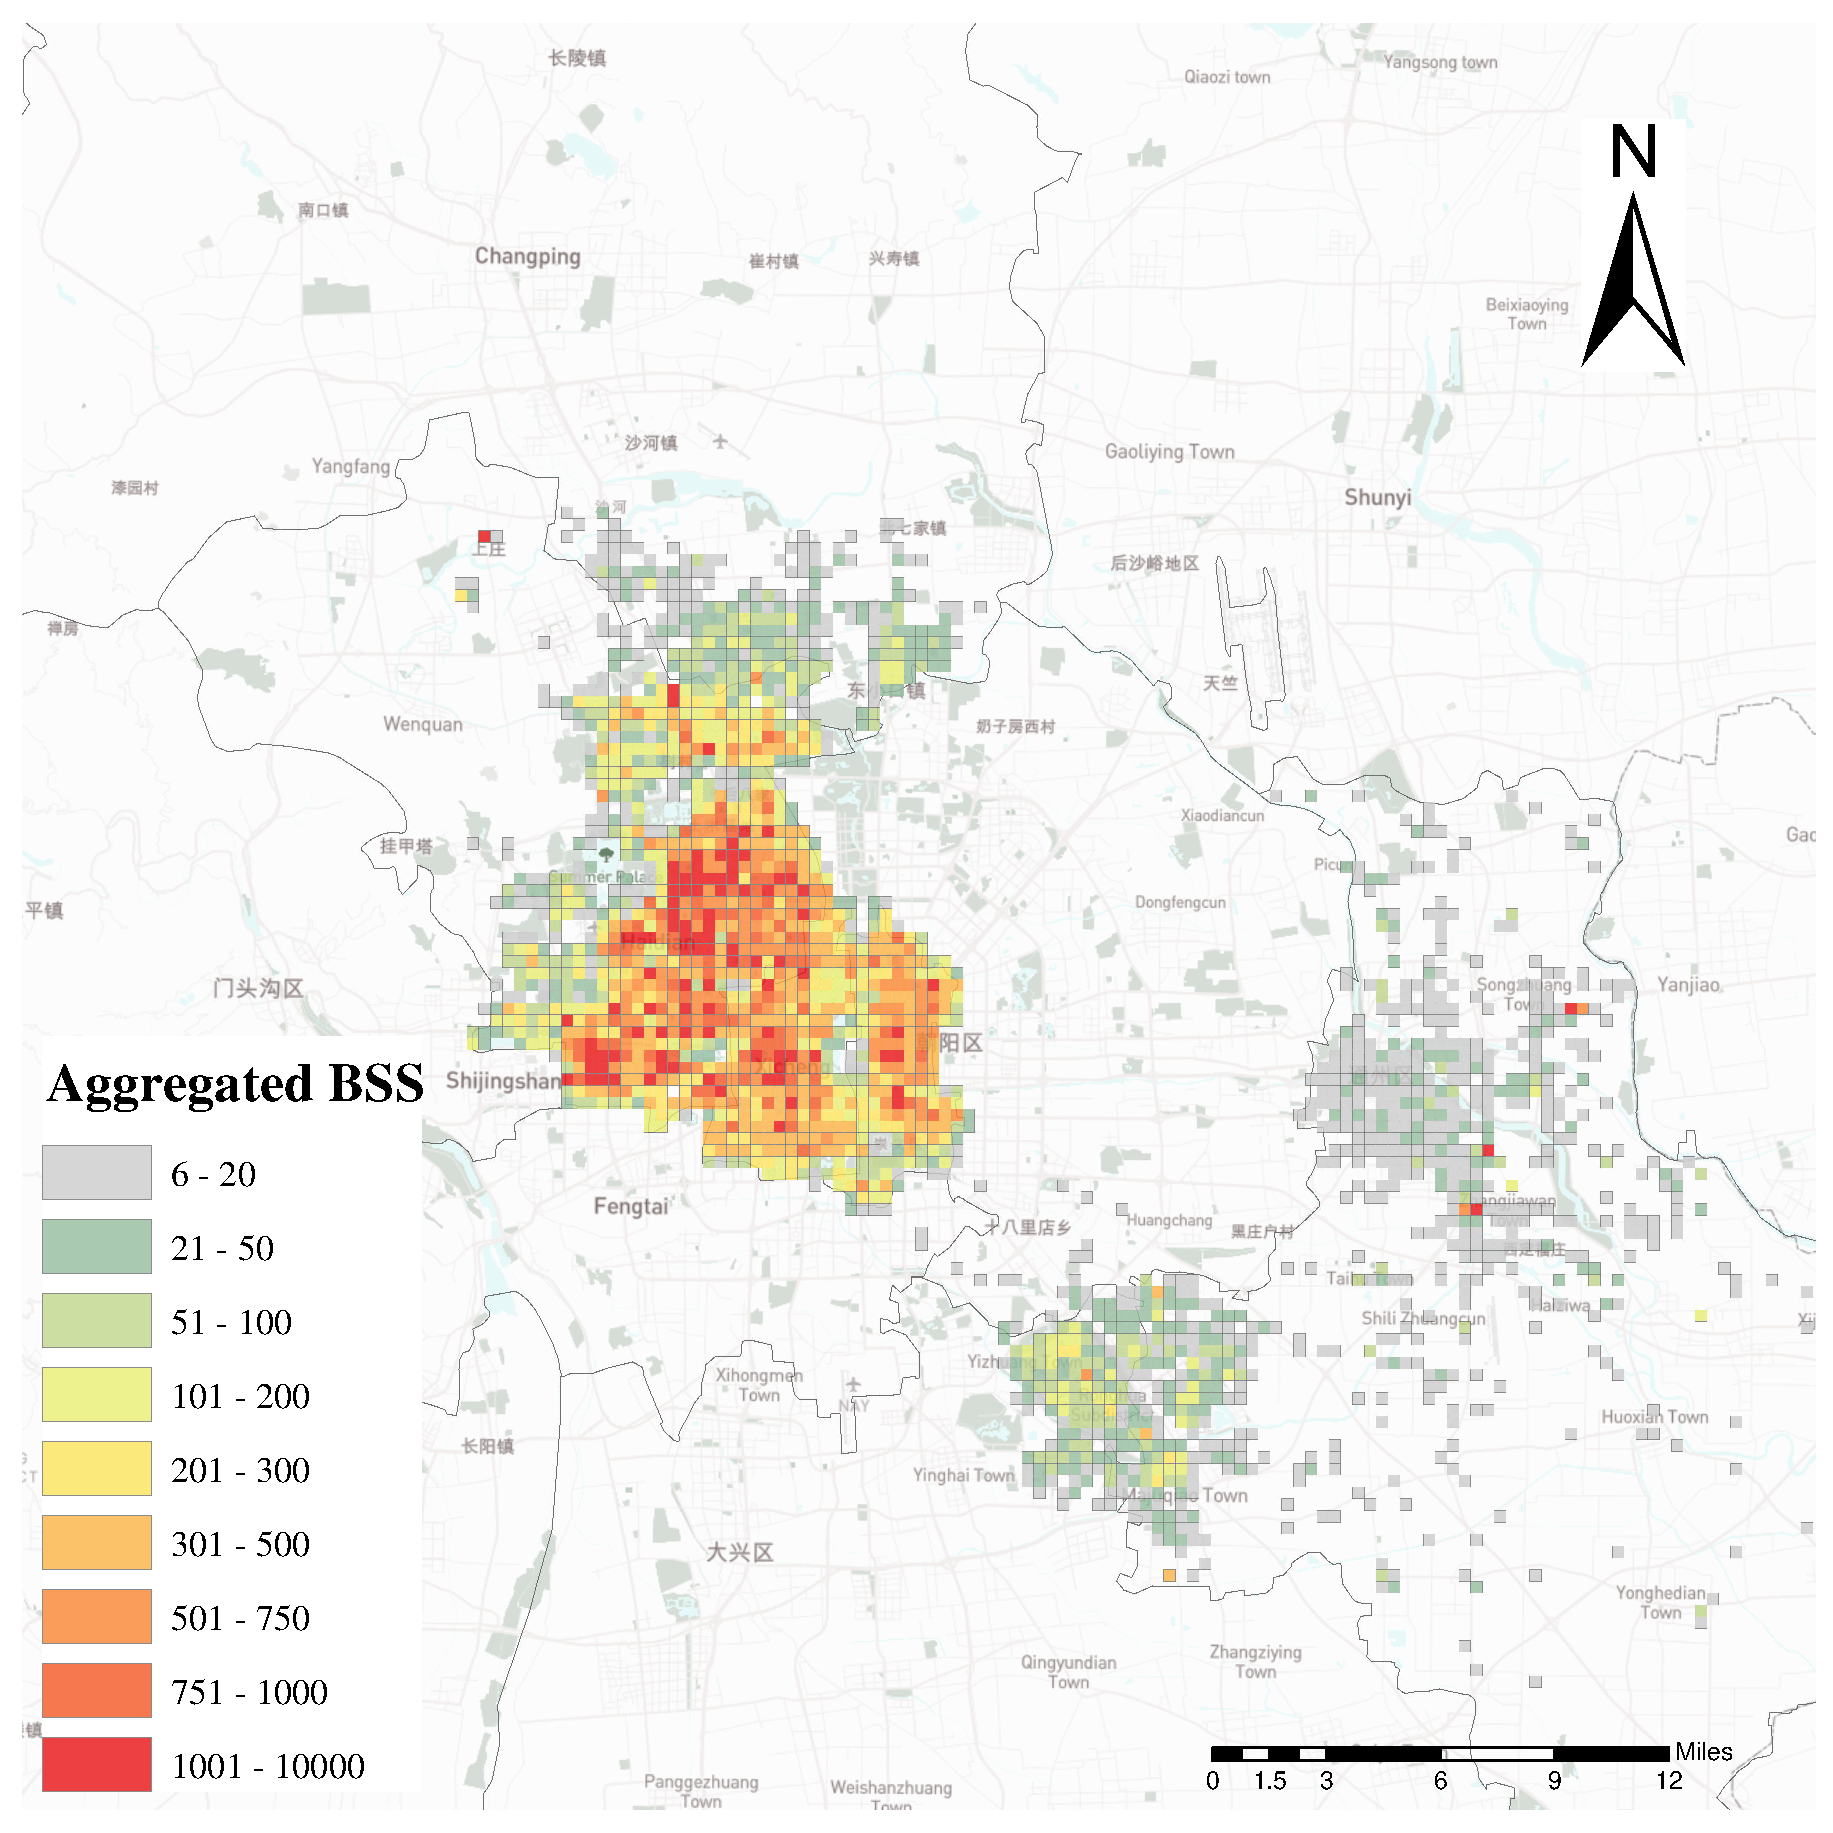
\includegraphics[width=\textwidth]{Figures/BSSPhase1_2020.eps}
        \caption{Phase a of 2020}
    \end{subfigure}
    \begin{subfigure}{.3\textwidth}
        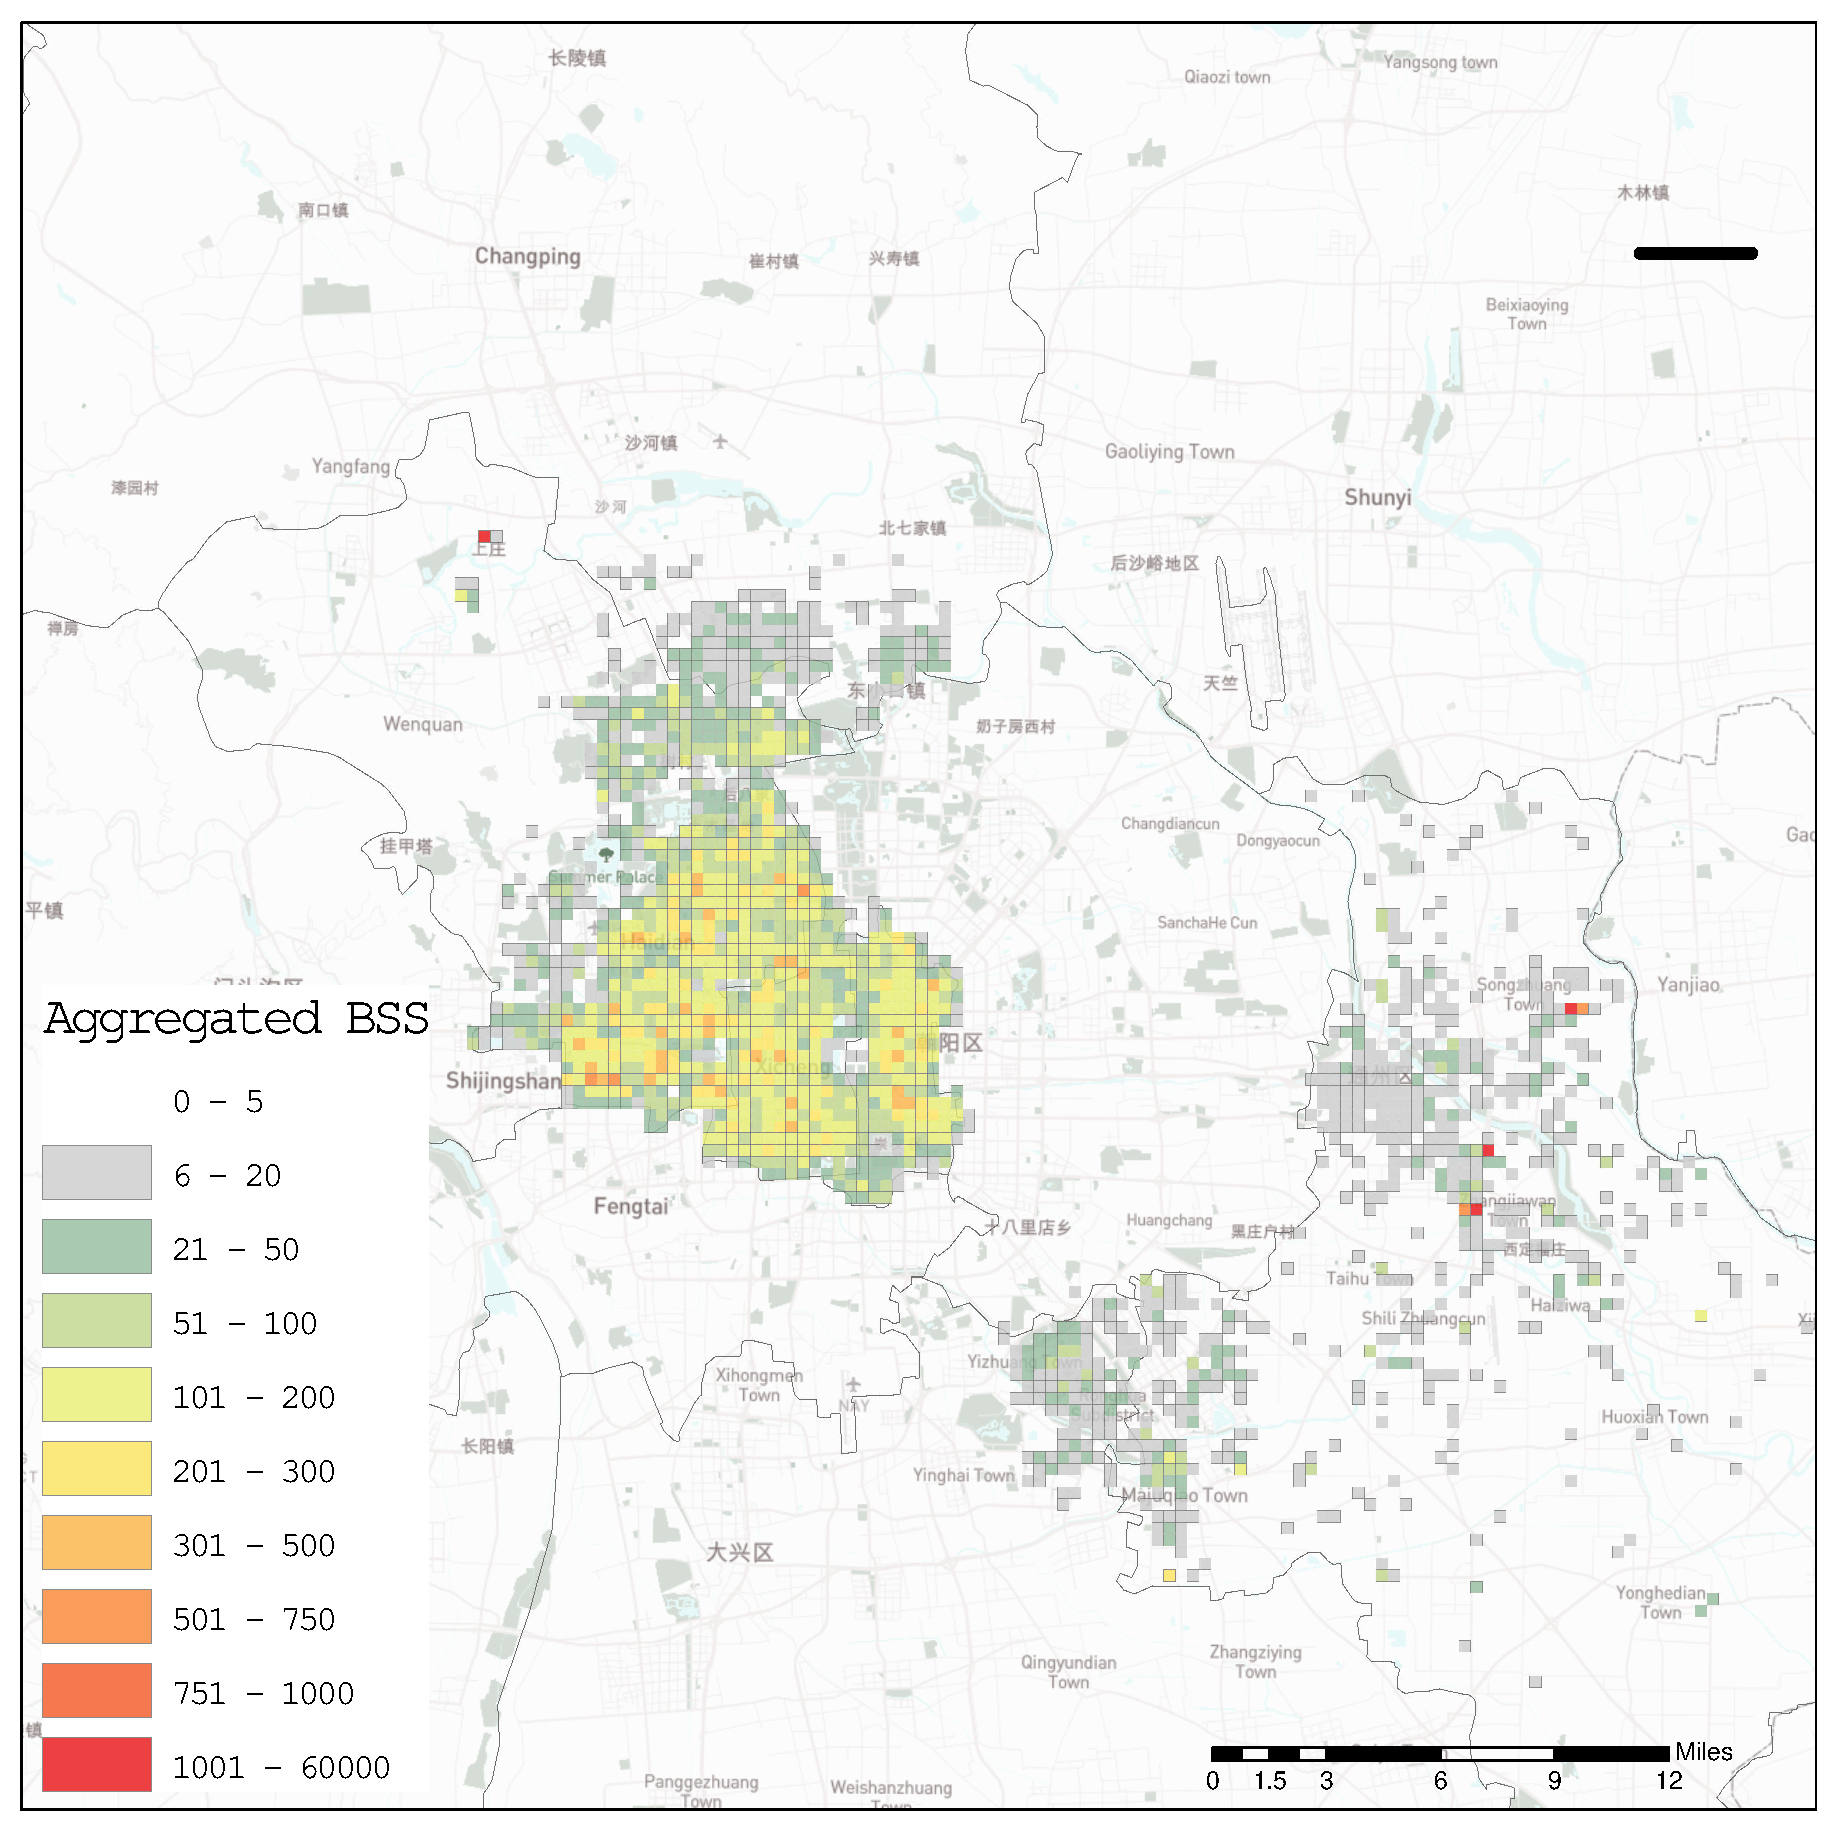
\includegraphics[width=\textwidth]{Figures/BSSPhase2_2020.eps}
        \caption{Phase b of 2020}
    \end{subfigure}
    \begin{subfigure}{.3\textwidth}
        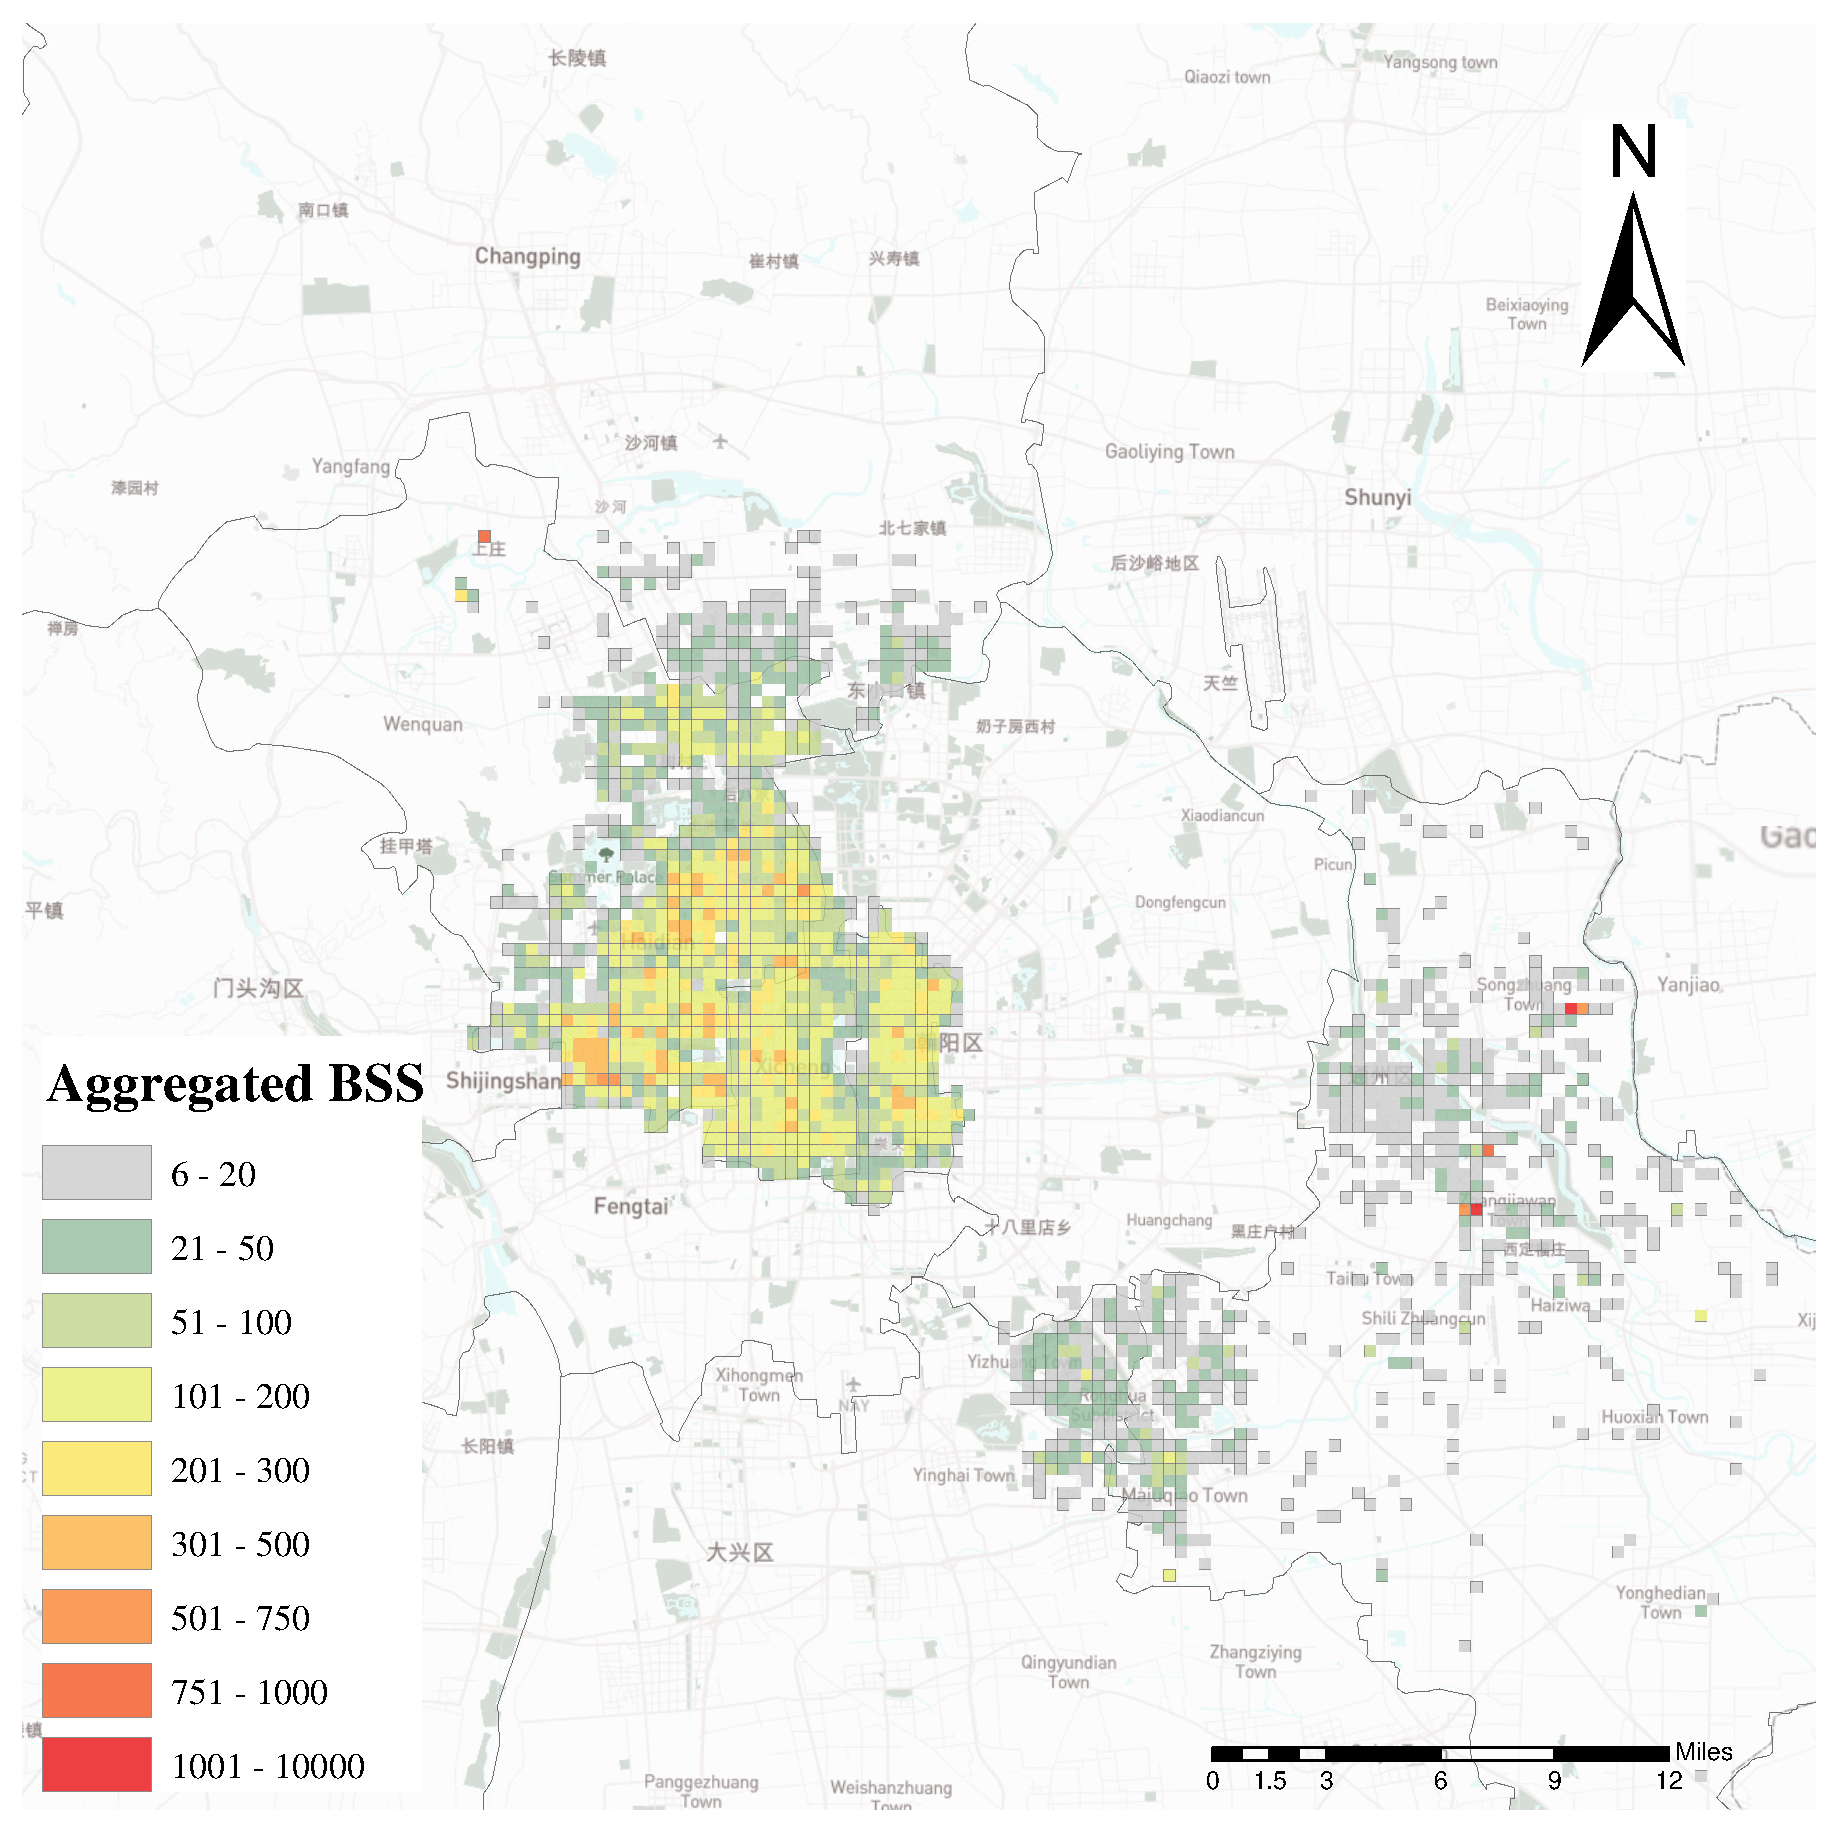
\includegraphics[width=\textwidth]{Figures/BSSPhase3_2020.eps}
        \caption{Phase c of 2020}
    \end{subfigure}
    
    \vspace{6pt}
    \begin{subfigure}{.3\textwidth}
        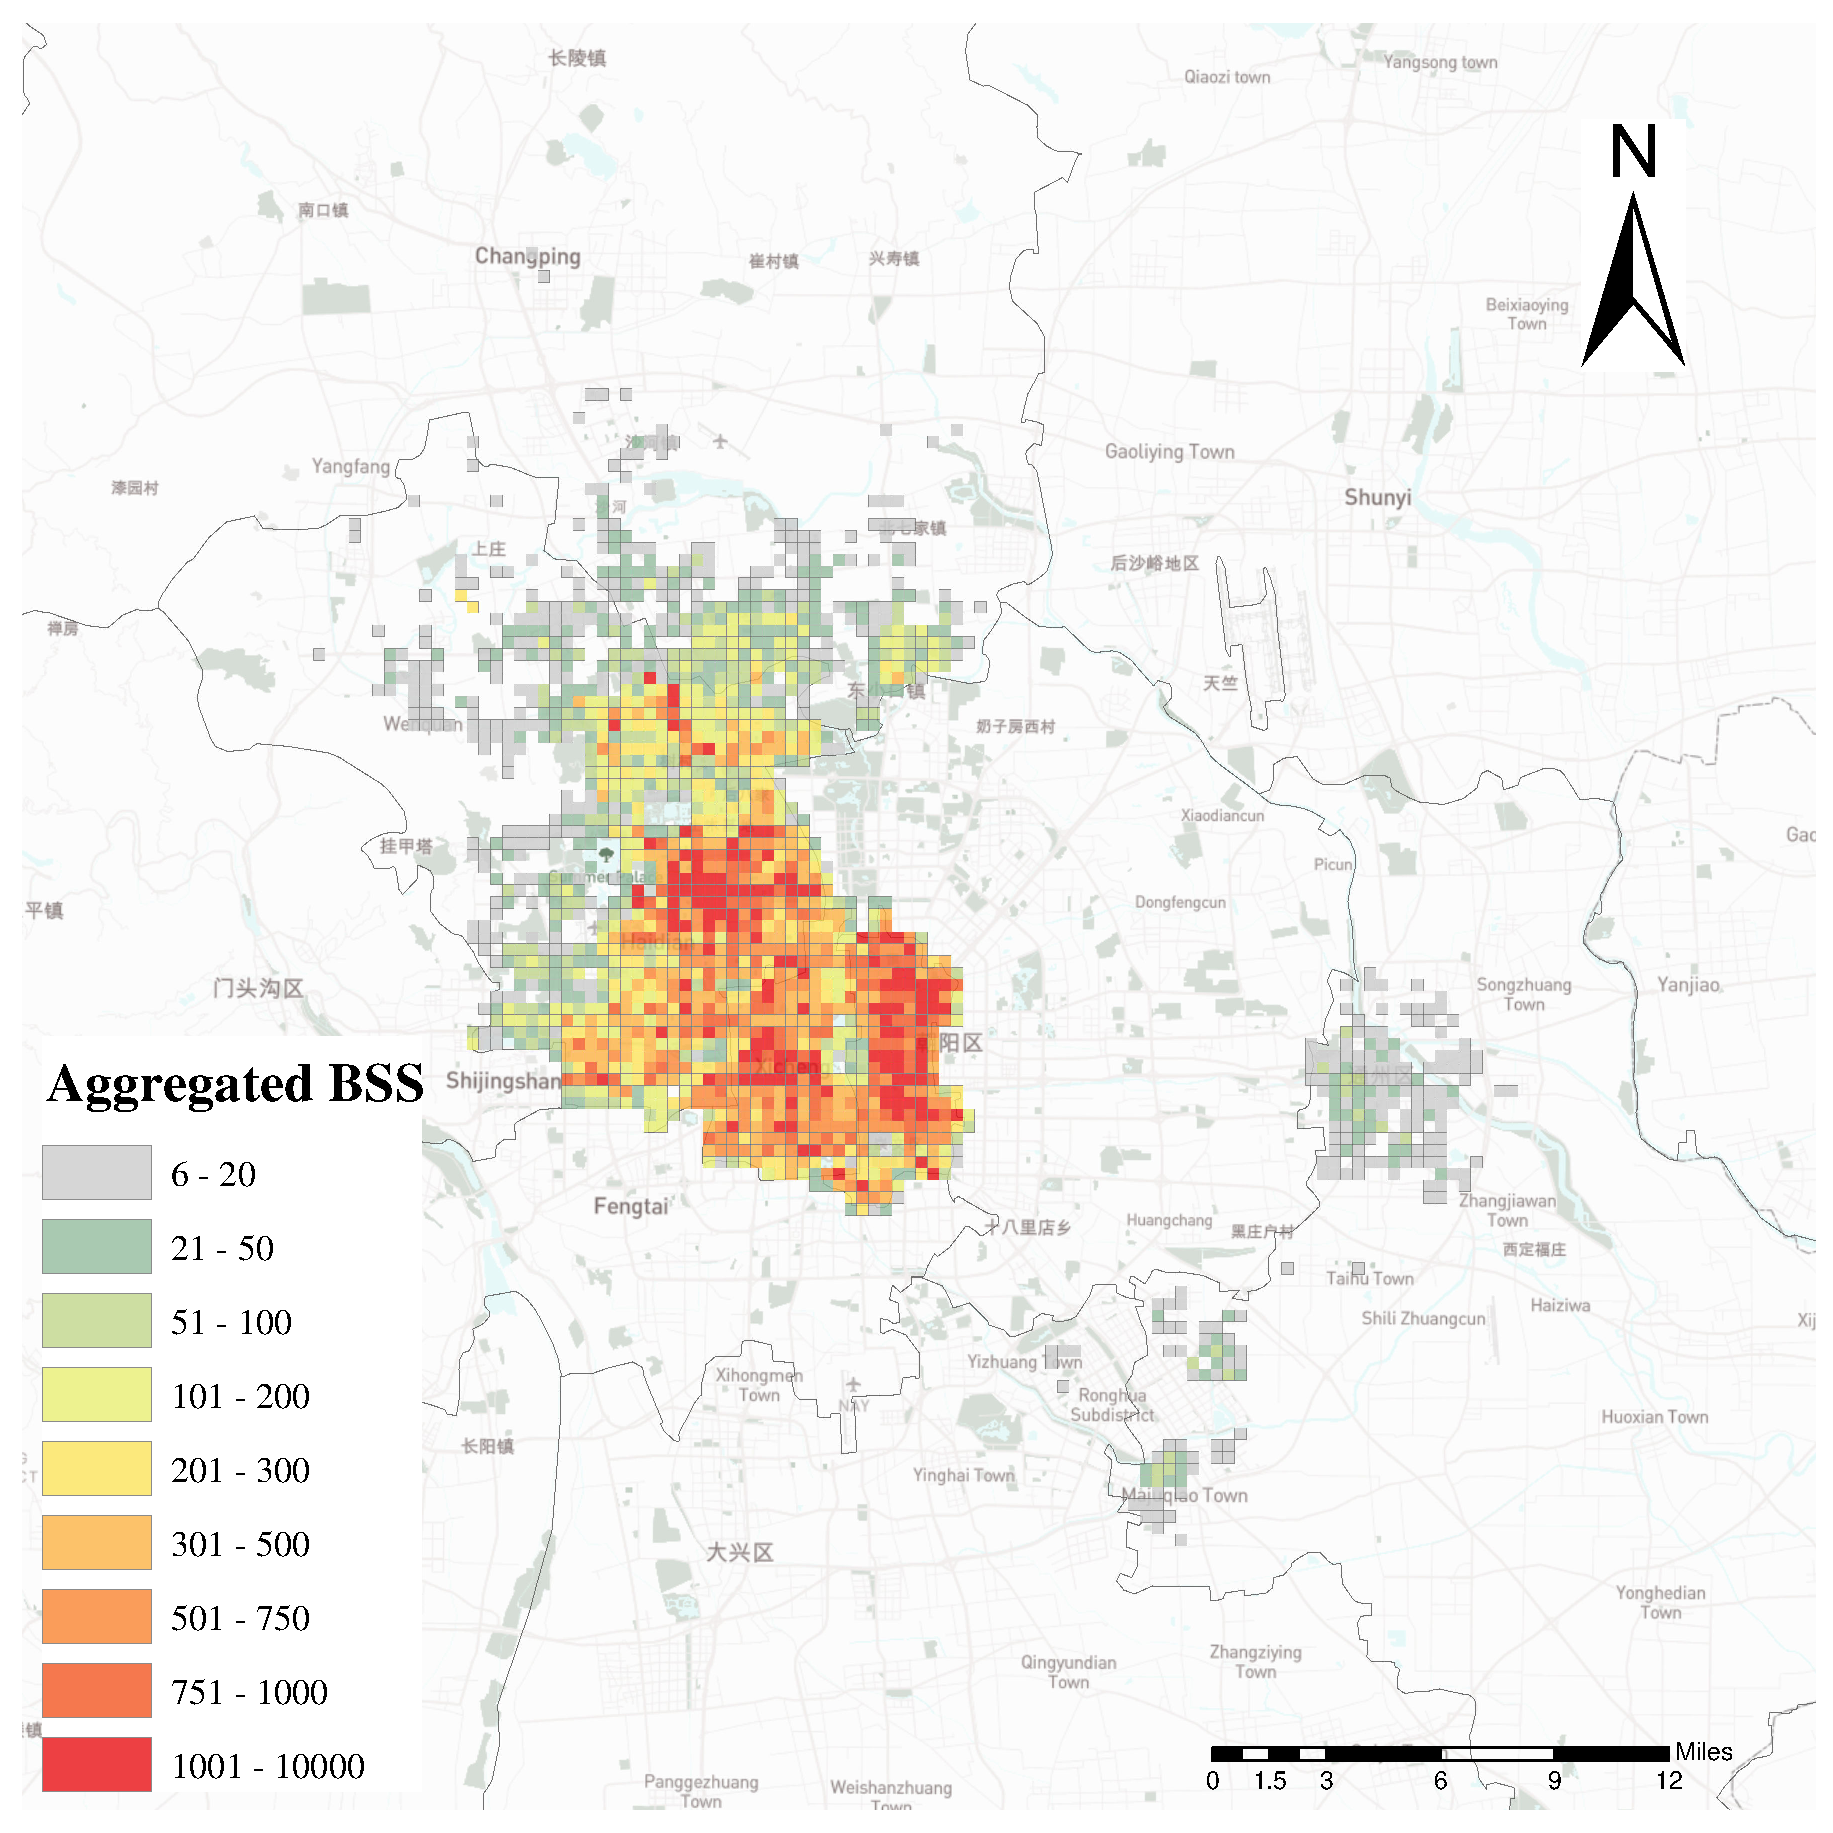
\includegraphics[width=\textwidth]{Figures/BSSPhase1_2019.eps}
        \caption{Phase a of 2019}
    \end{subfigure}
    \begin{subfigure}{.3\textwidth}
        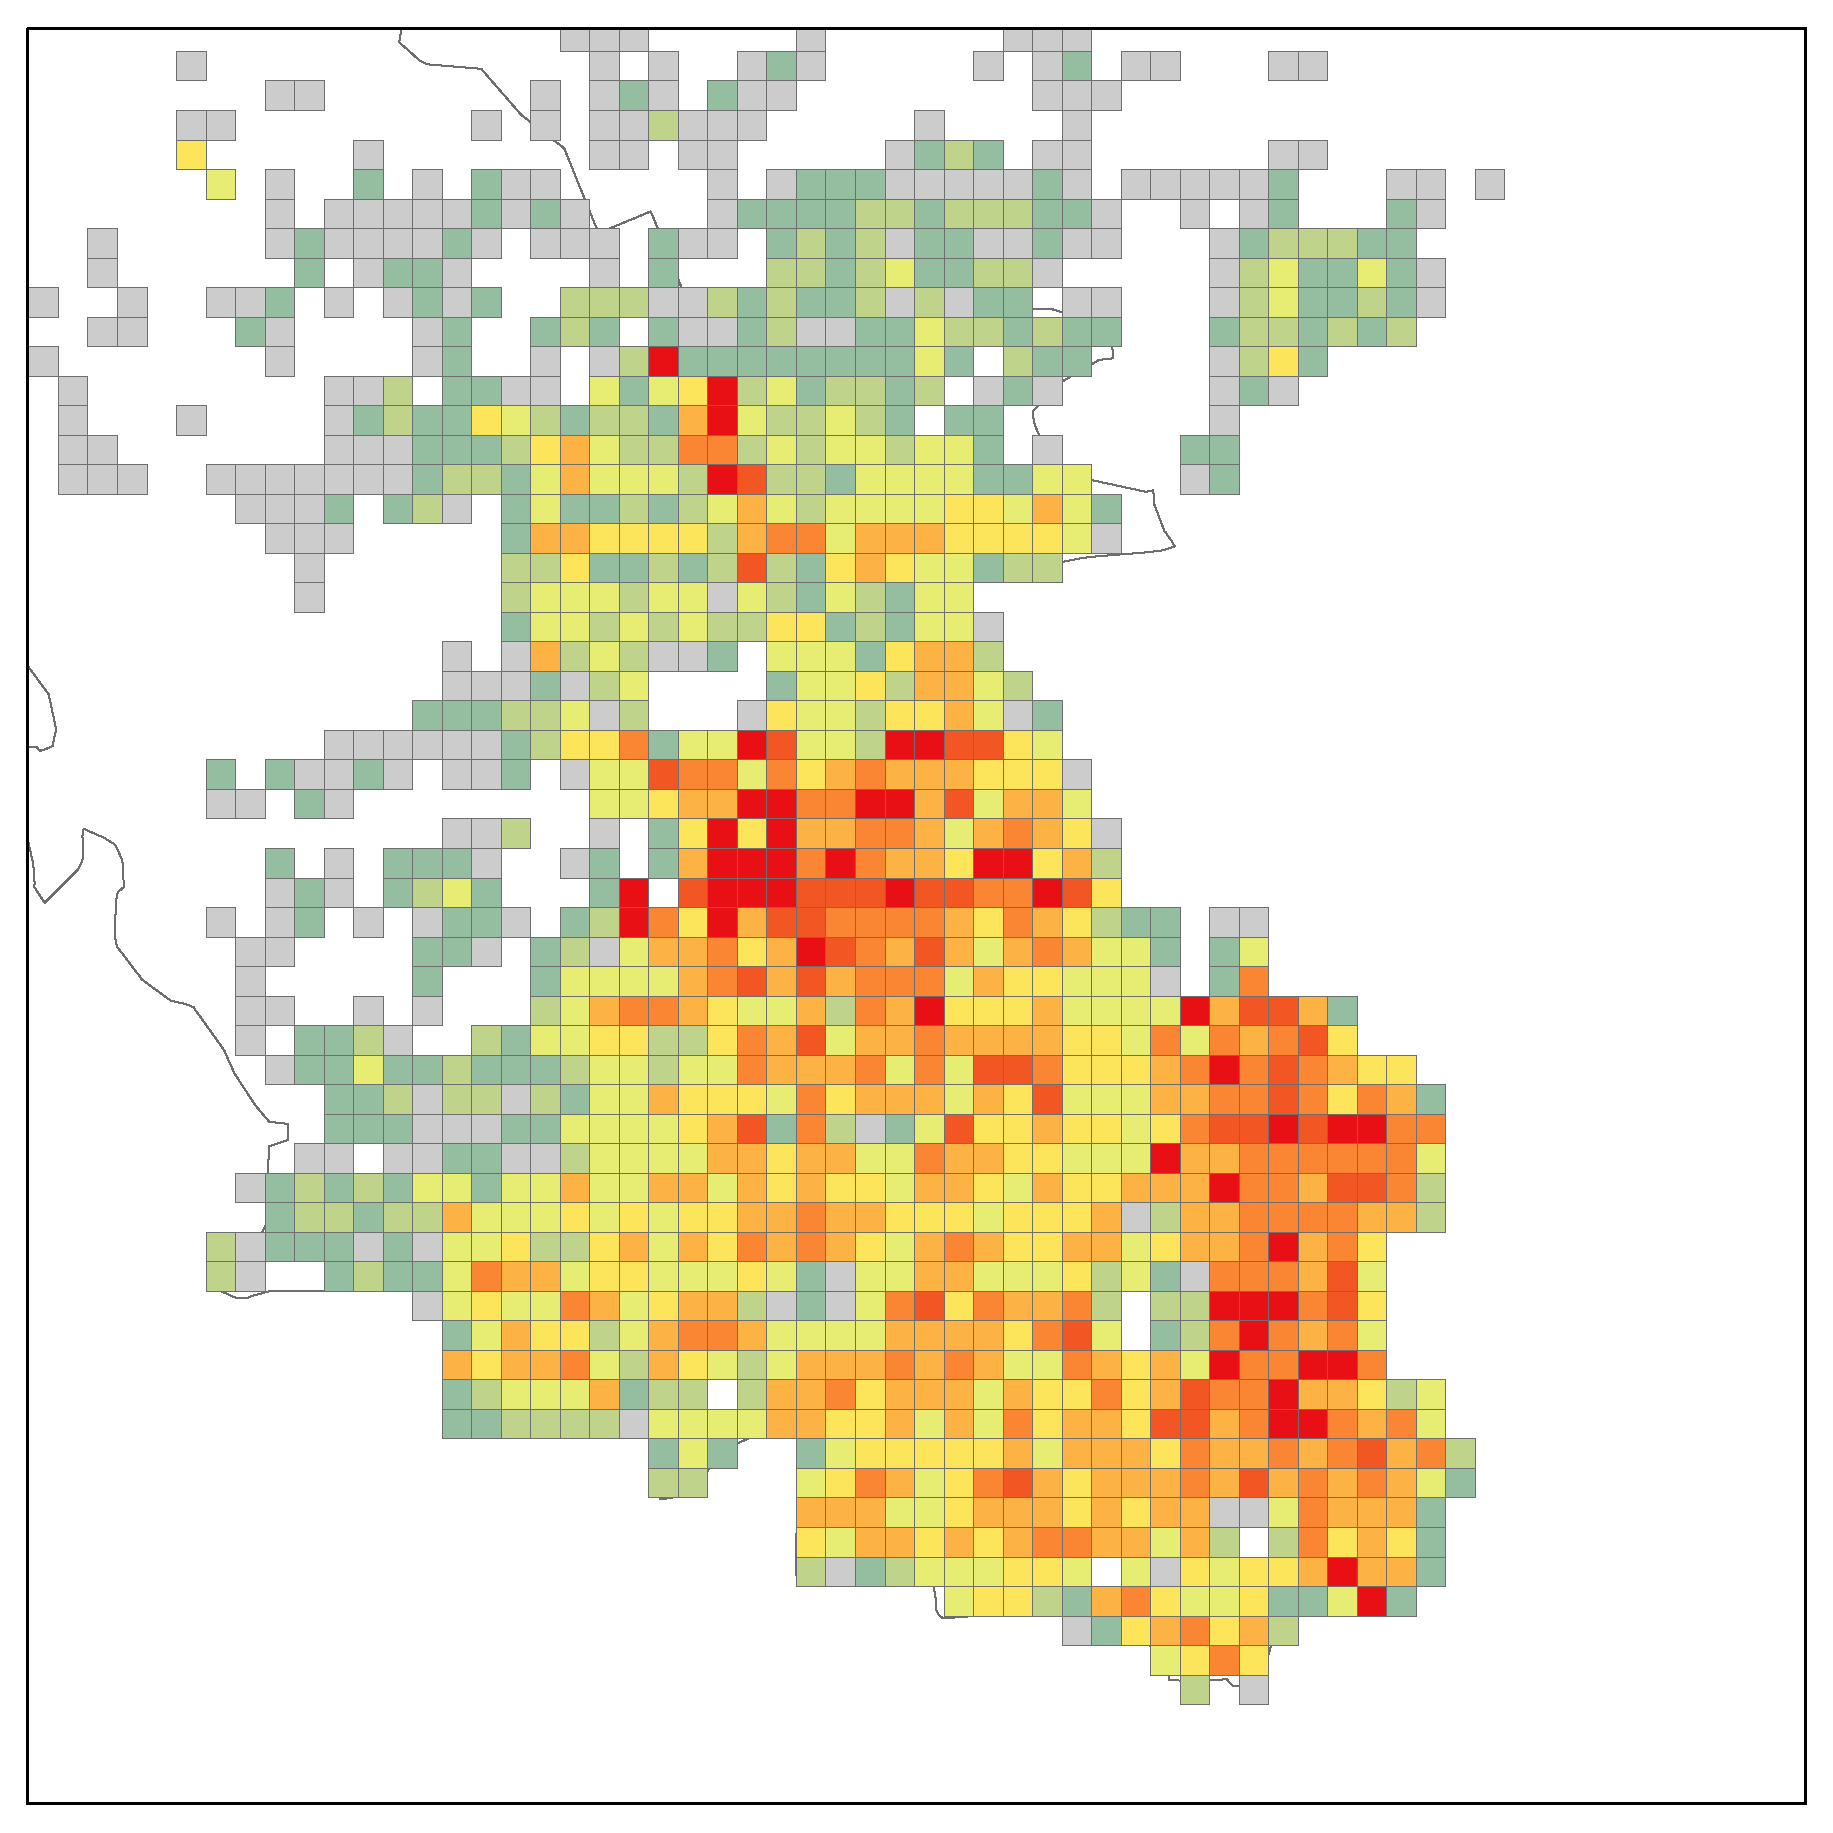
\includegraphics[width=\textwidth]{Figures/BSSPhase2_2019.eps}
        \caption{Phase b of 2019}
    \end{subfigure}
    \begin{subfigure}{.3\textwidth}
        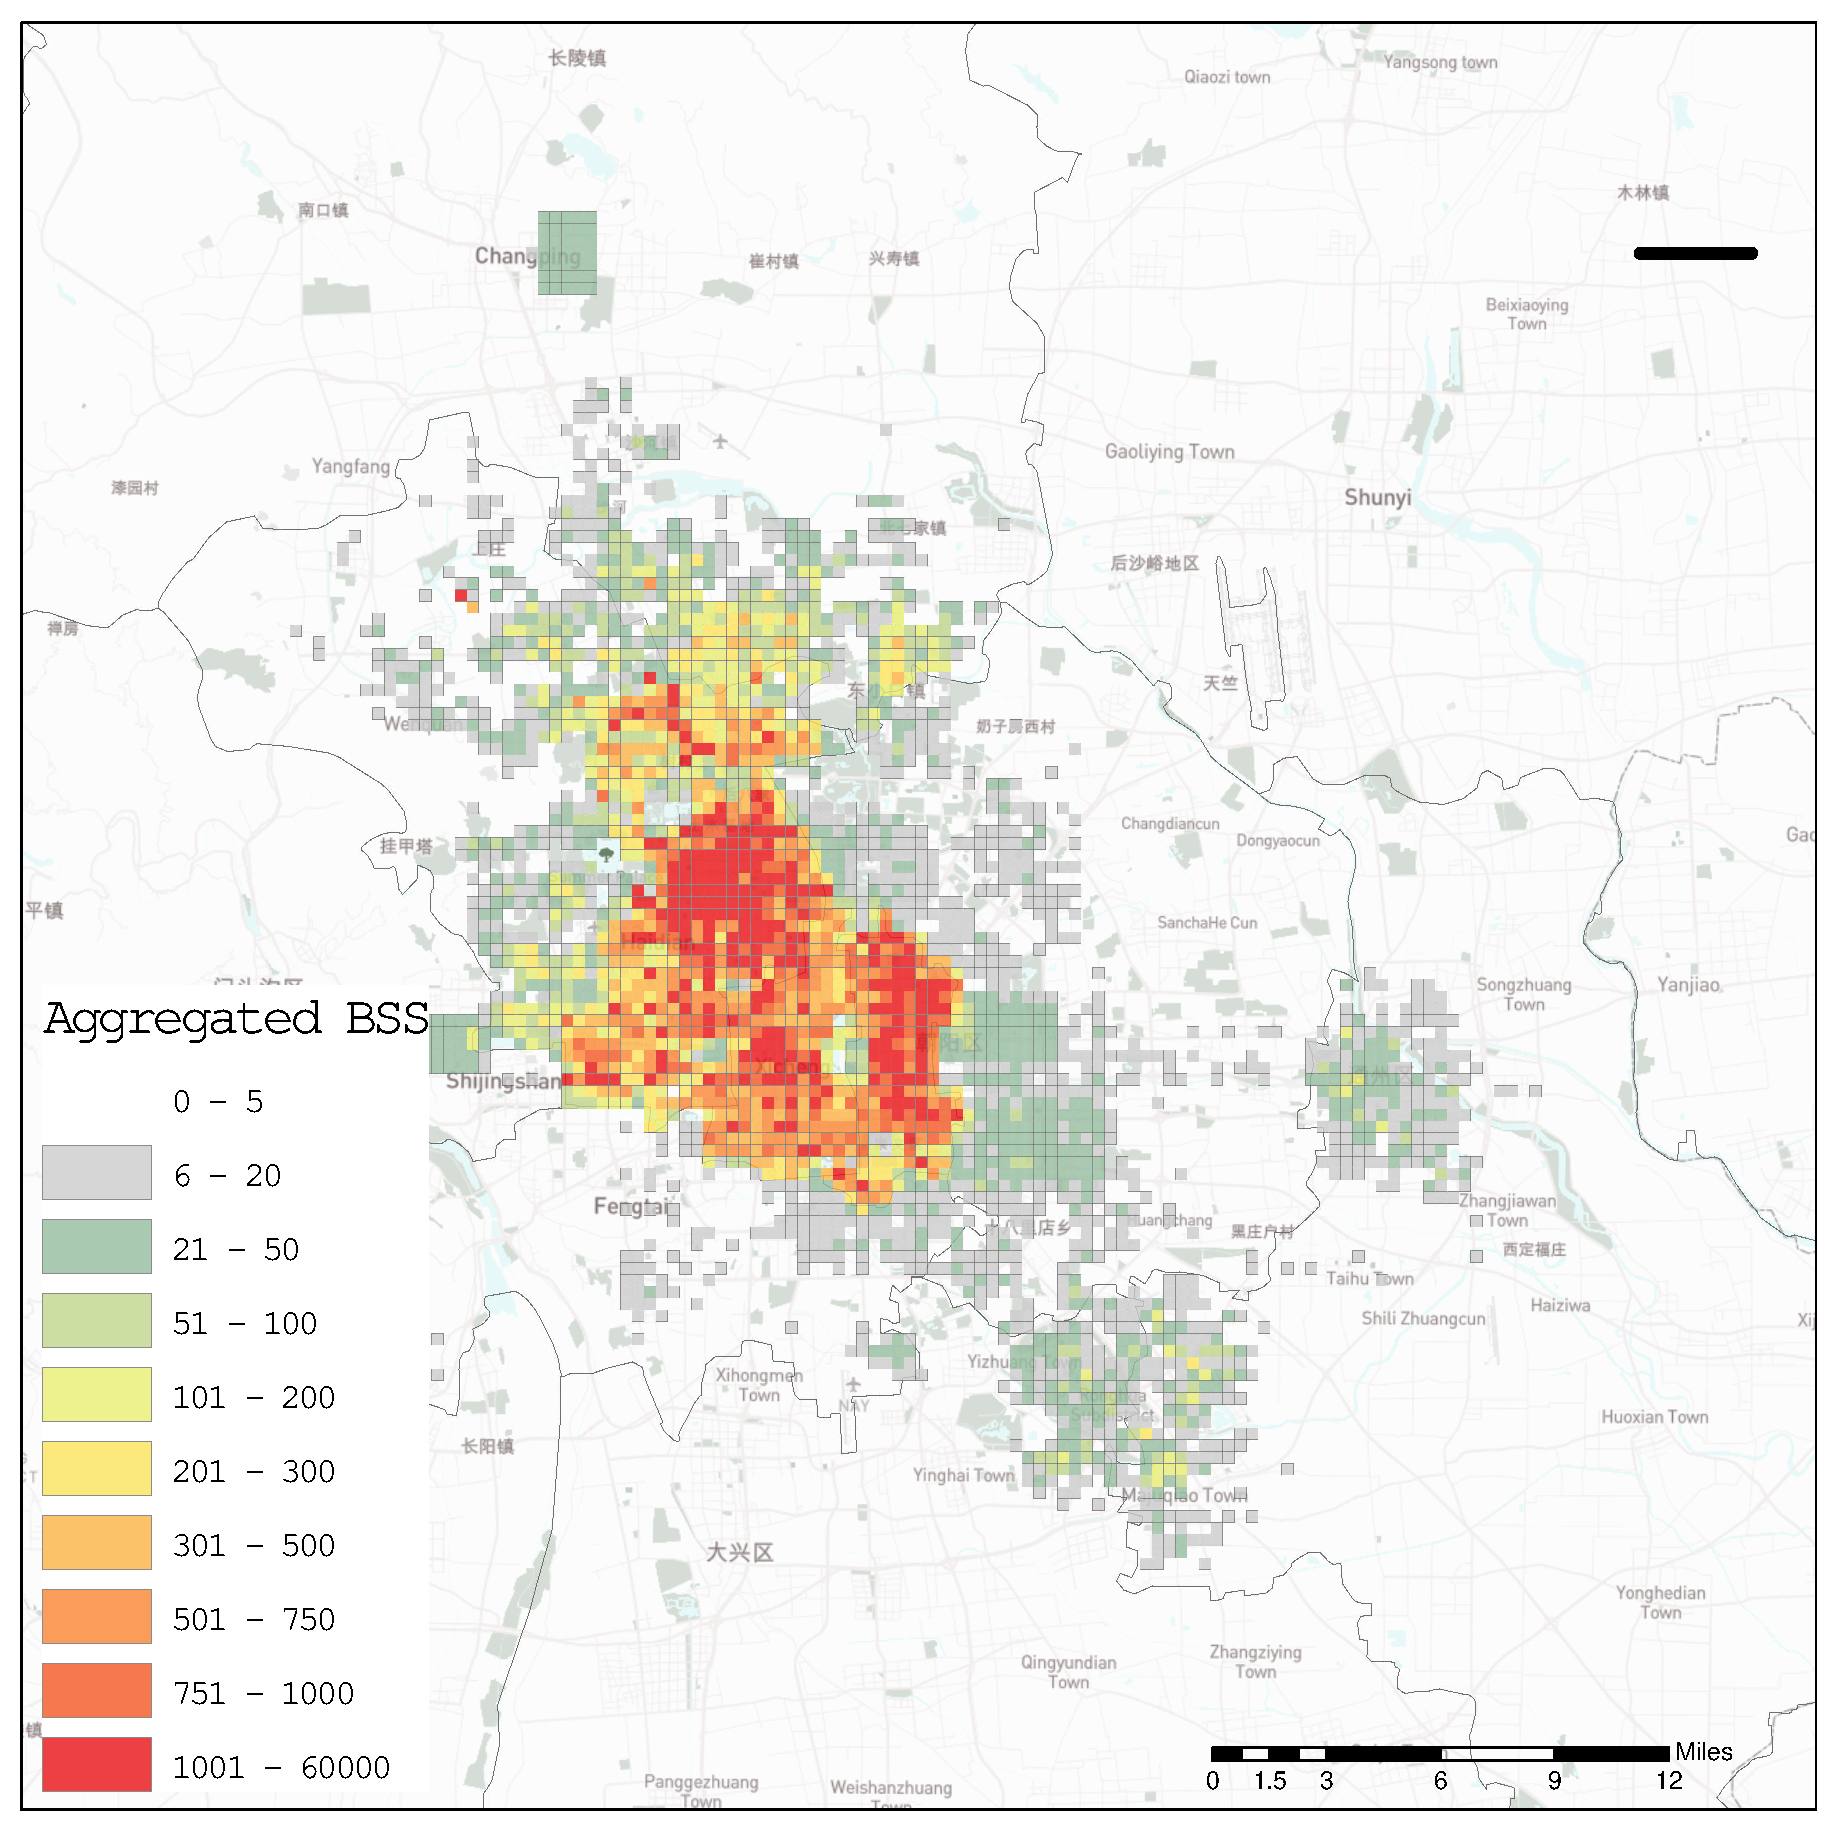
\includegraphics[width=\textwidth]{Figures/BSSPhase3_2019.eps}
        \caption{Phase c of 2019}
    \end{subfigure}
    
    \vspace{6pt}
    \begin{subfigure}{.3\textwidth}
        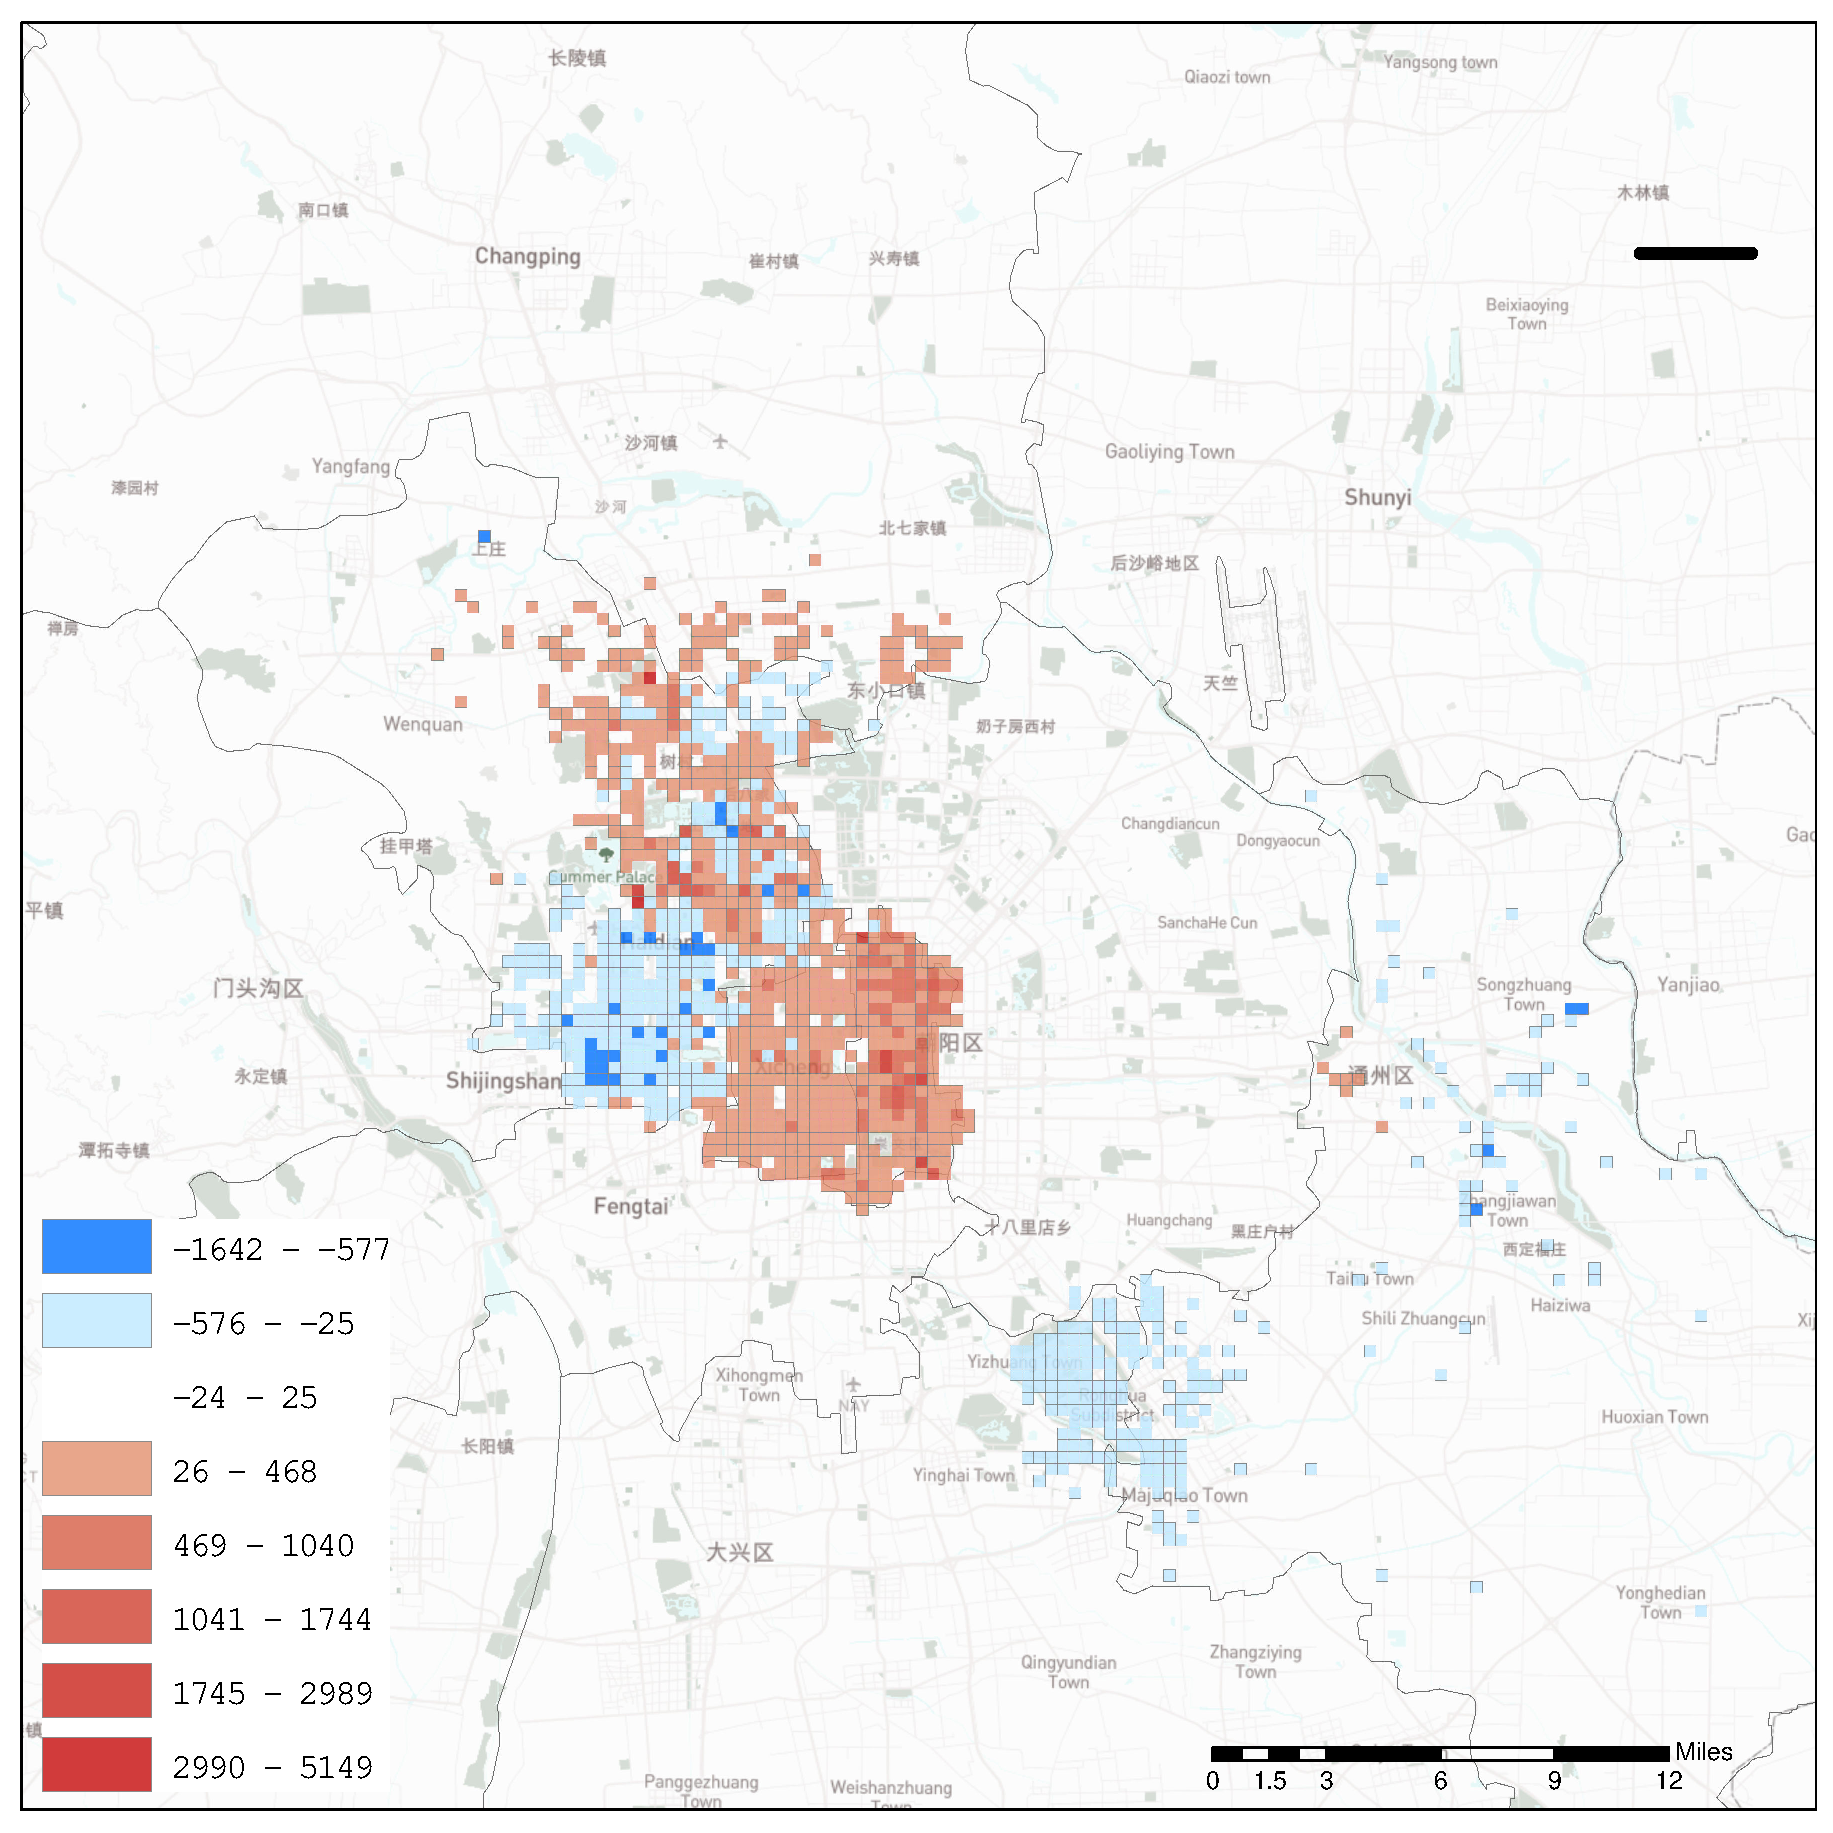
\includegraphics[width=\textwidth]{Figures/BSSMinusmp1.eps}
        \caption{Differential image of Phase a}
    \end{subfigure}
        \begin{subfigure}{.3\textwidth}
        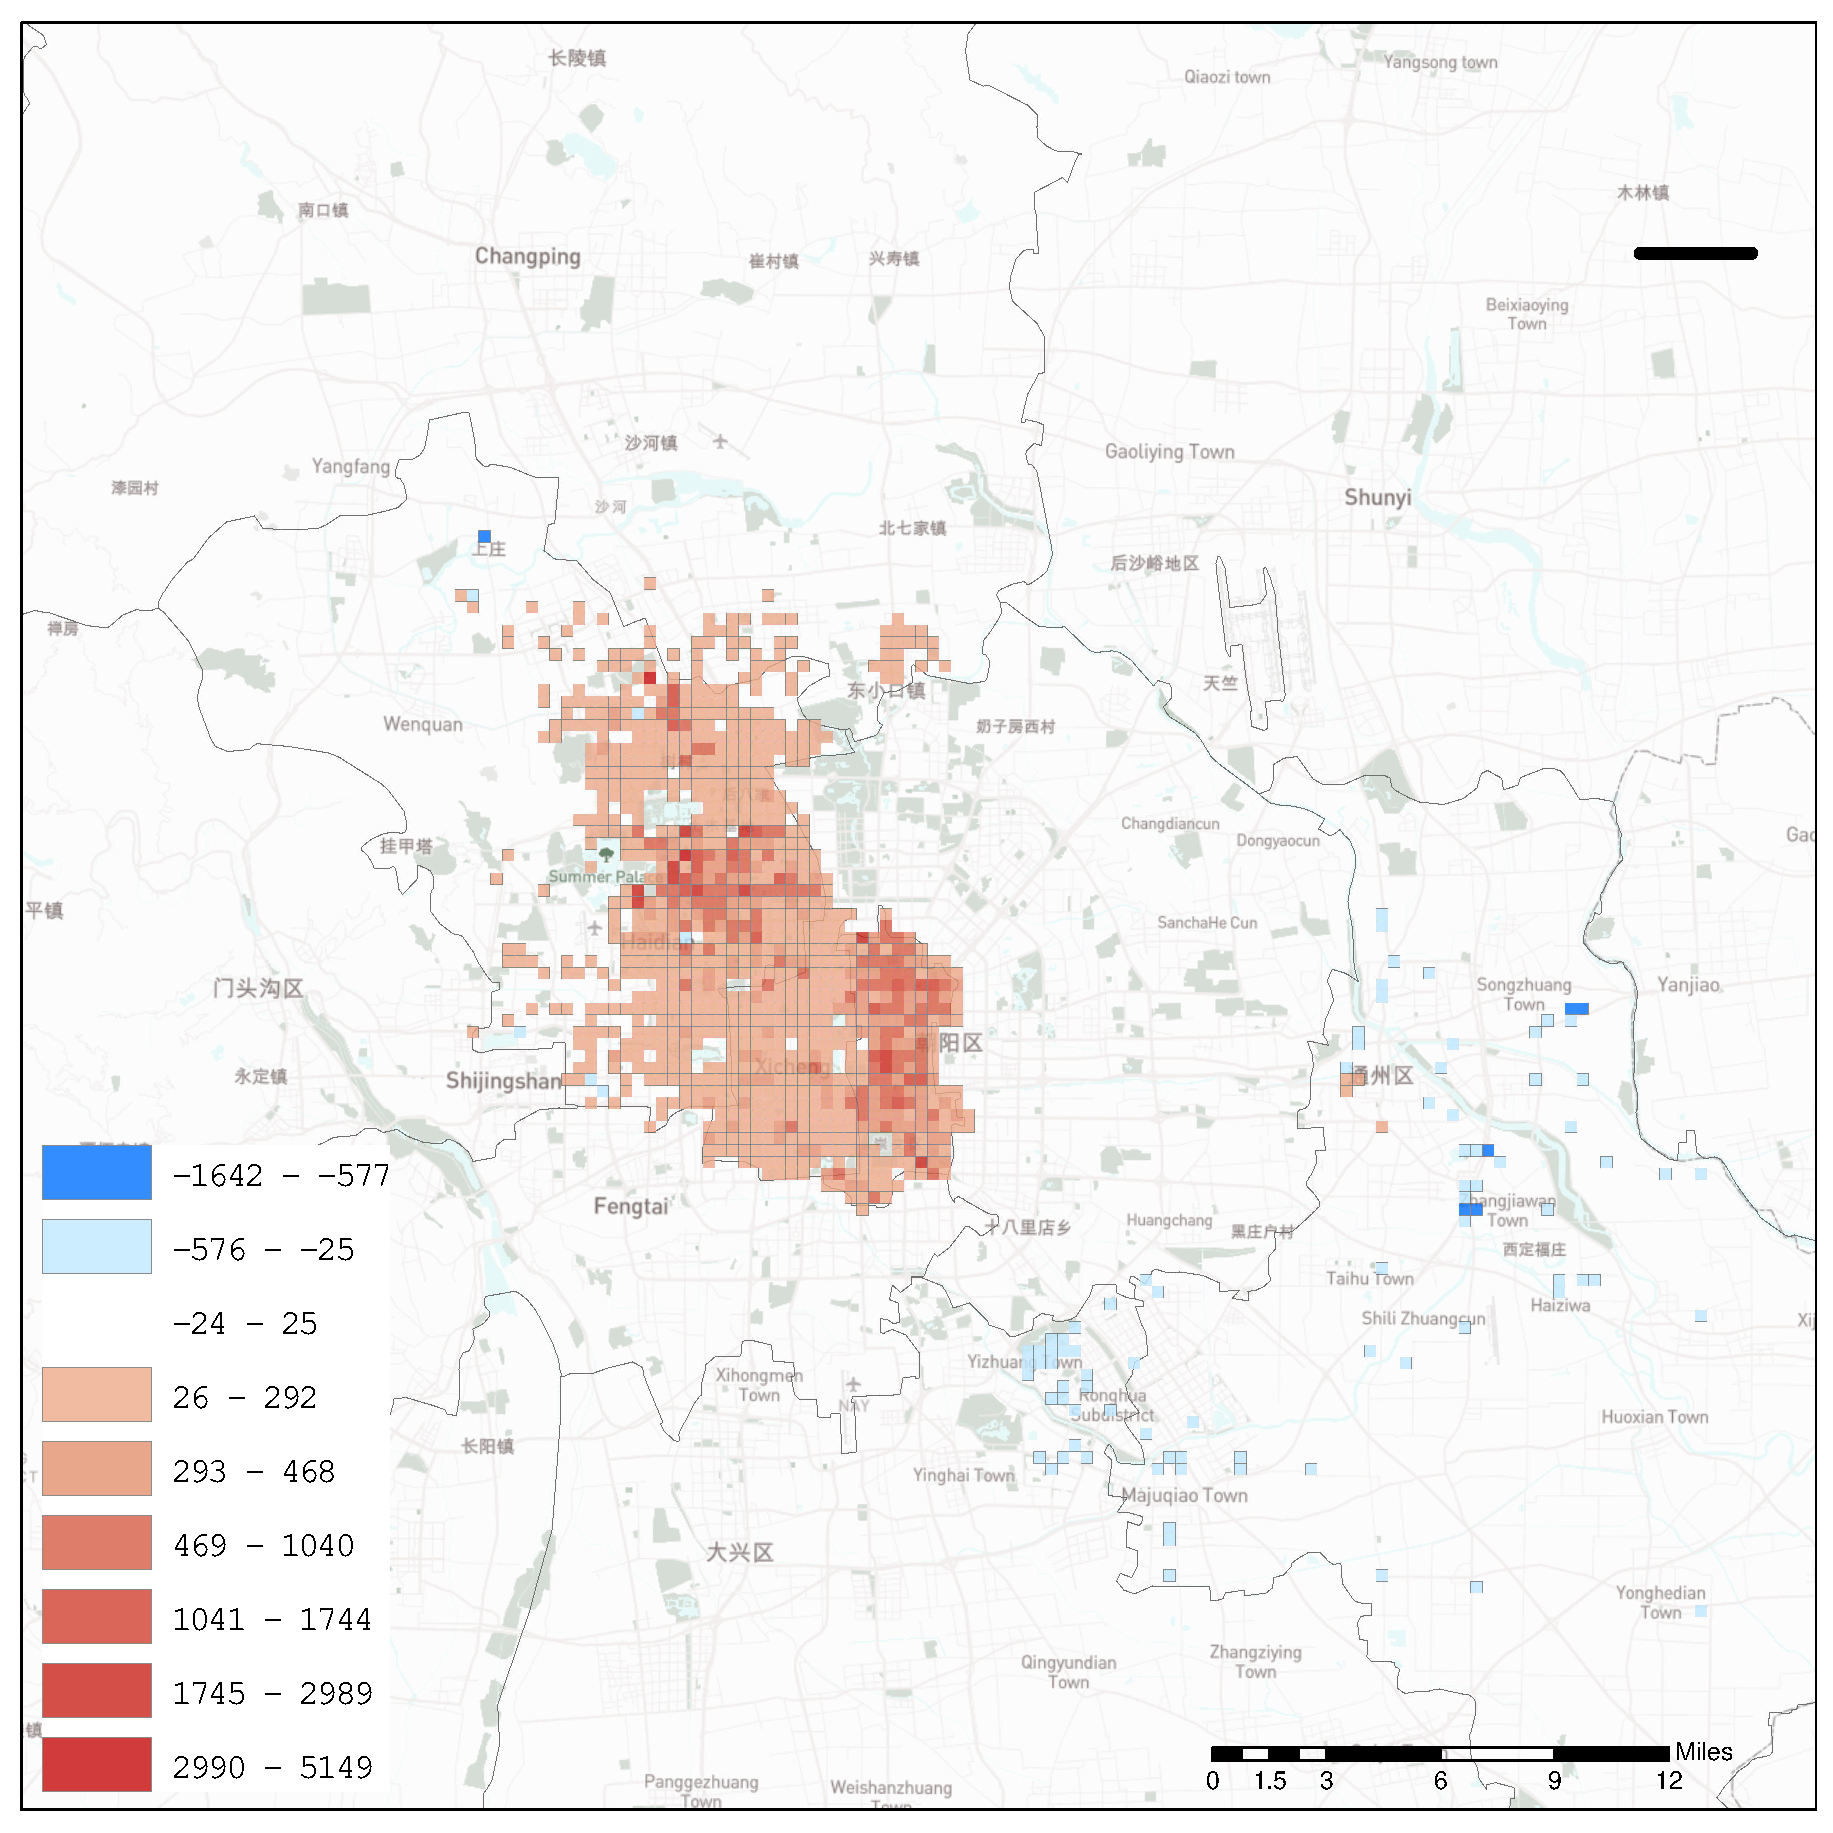
\includegraphics[width=\textwidth]{Figures/BSSMinusmp2.eps}
        \caption{Differential image of Phase b}
    \end{subfigure}
        \begin{subfigure}{.3\textwidth}
        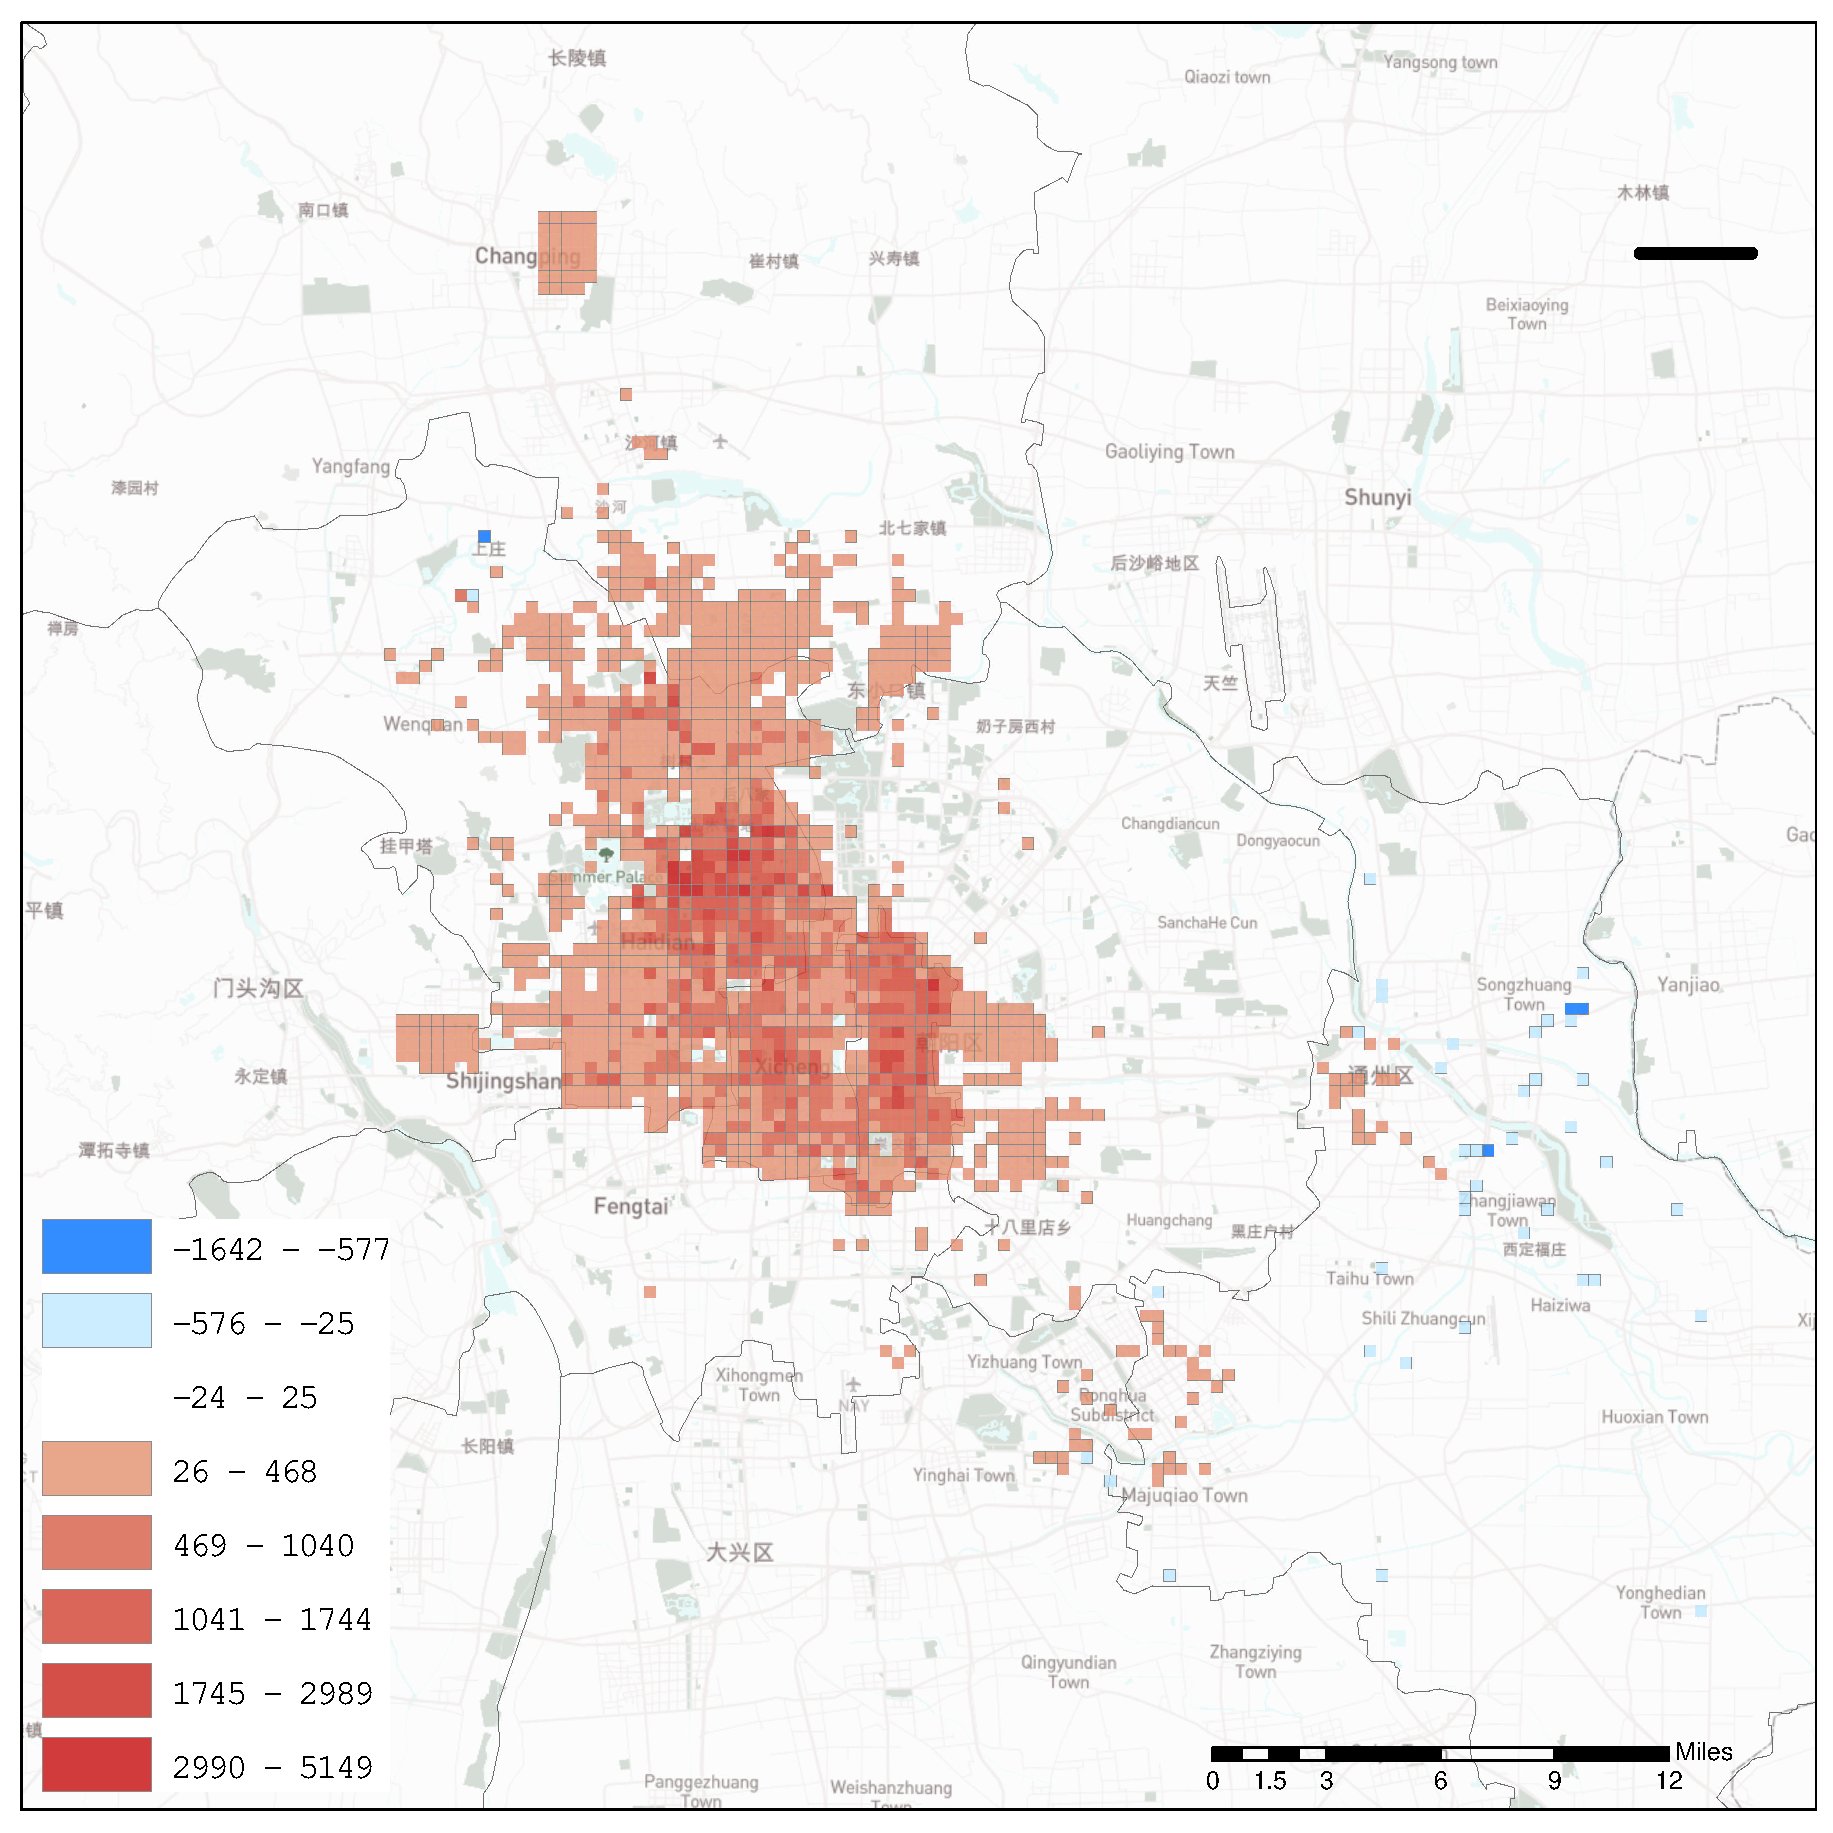
\includegraphics[width=\textwidth]{Figures/BSSMinusmp3.eps}
        \caption{Differential image of Phase c}
    \end{subfigure}
    \caption{Caption}
    \label{fig:compare_2019_and_2020}
\end{figure}

Figure \ref{fig:compare_2019_and_2020} delineates the results corresponding to 2020, 2019, and annual difference in between.
Panel (a) - (c) were consistent with the daily patterns during different pandemic stages presented in the previous section.
Panel (d) - (f) summarized the averaged share bike intensity during the same time-interval as \textbf{phase a} in 2019, showing similar spatial patterns as 2020. 
In Panel (g) - (i), (Comparable numbers of positive (Red colored) and negative (blue colored) area could be observed from annual difference presented in panel (g). These discrepancies have relatively low values which could be attributed to the fluctuation of regional bike usages requirements.  

The significant discrepancies in share bike usage between year 2019 and 2020 during \textbf{phase b} and \textbf{phase c} is considered as the consequence of the pandemic of COVID-19. 
Normally, most migrants ($34.6\%$ of the population of Beijing) go back to their hometown during Chinese New Year holiday; while permanent residents enjoy family gathering and the main outdoor activity is visiting relatives and friends.
Therefore the holidays shutdowns reduced mobility in 2019, but high-intensity mobility could still be found in the urban districts from panel (e). 
Correspondingly, activities were in a state of complete suppression in 2020. 
The difference map in panel (h) reveals the fact that under the impact of COVID-19, demands for outings were reduced for safe purposes.

In previous years, panel (f) indicated that mobility would instantly return to pre-festival levels or more widespread as a result of the influx of migrant workers after holiday.
According to panel (c), the rehabilitation was in progress, but much slower during epidemic mitigated period.
The remarkable difference referred from panel (i) verified this sustained impact on the daily lives of citizens.

\subsection{Relevance between cycling activities and confirmed cases during epidemic phase} 

This part aims at characterizing the behavior patterns of disease-spreading individuals by evaluating share bike usages with respect to different pandemic periods.%thus provide reference for authorities to gradually lift the most restrictive measures with more precision and confidence.

Figure \ref{fig:BSS_phase1_2} shows the share bike usages in \textbf{phase b}, \textit{i.e.} the quanratine period.
Same as previous sections, aggregated share bike records were rendered with a color ramp from grey to green to red.
Confirmed cases in each district are displayed by blue circles, where the cumulative number of cases is shown by the size of circles.
When comparing the panels from left to right with date varying from 25 Jan to 08 Feb, we observe that the aggregated share bike intensity gradually decreases with increasing number of confirmed cases and then remains at low level.
The aggregated share bike intensity in downtown area changed from red to green.
%The reason could be attributed to the individuals' response against the high infectious risk and government's measures.
Starting on January 25, 2020, highly restrictive measures were implemented by local government: individuals were asked to follow a series of social distancing measures.
As a result, the number of newly confirmed COVID-19 cases was effectively suppressed.

\begin{figure}[ht]
    \centering
    \begin{subfigure}{.3\textwidth}
        \includegraphics[width=\textwidth]{Figures/Relation_with_confrimed_cases/NewDistrictSSBD2020_01_21.eps}
        \caption{21 Jan}
    \end{subfigure}
    \begin{subfigure}{.3\textwidth}
        \includegraphics[width=\textwidth]{Figures/Relation_with_confrimed_cases/NewDistrictSSBD2020_01_25.eps}
        \caption{25 Jan}
    \end{subfigure}
    \begin{subfigure}{.3\textwidth}
        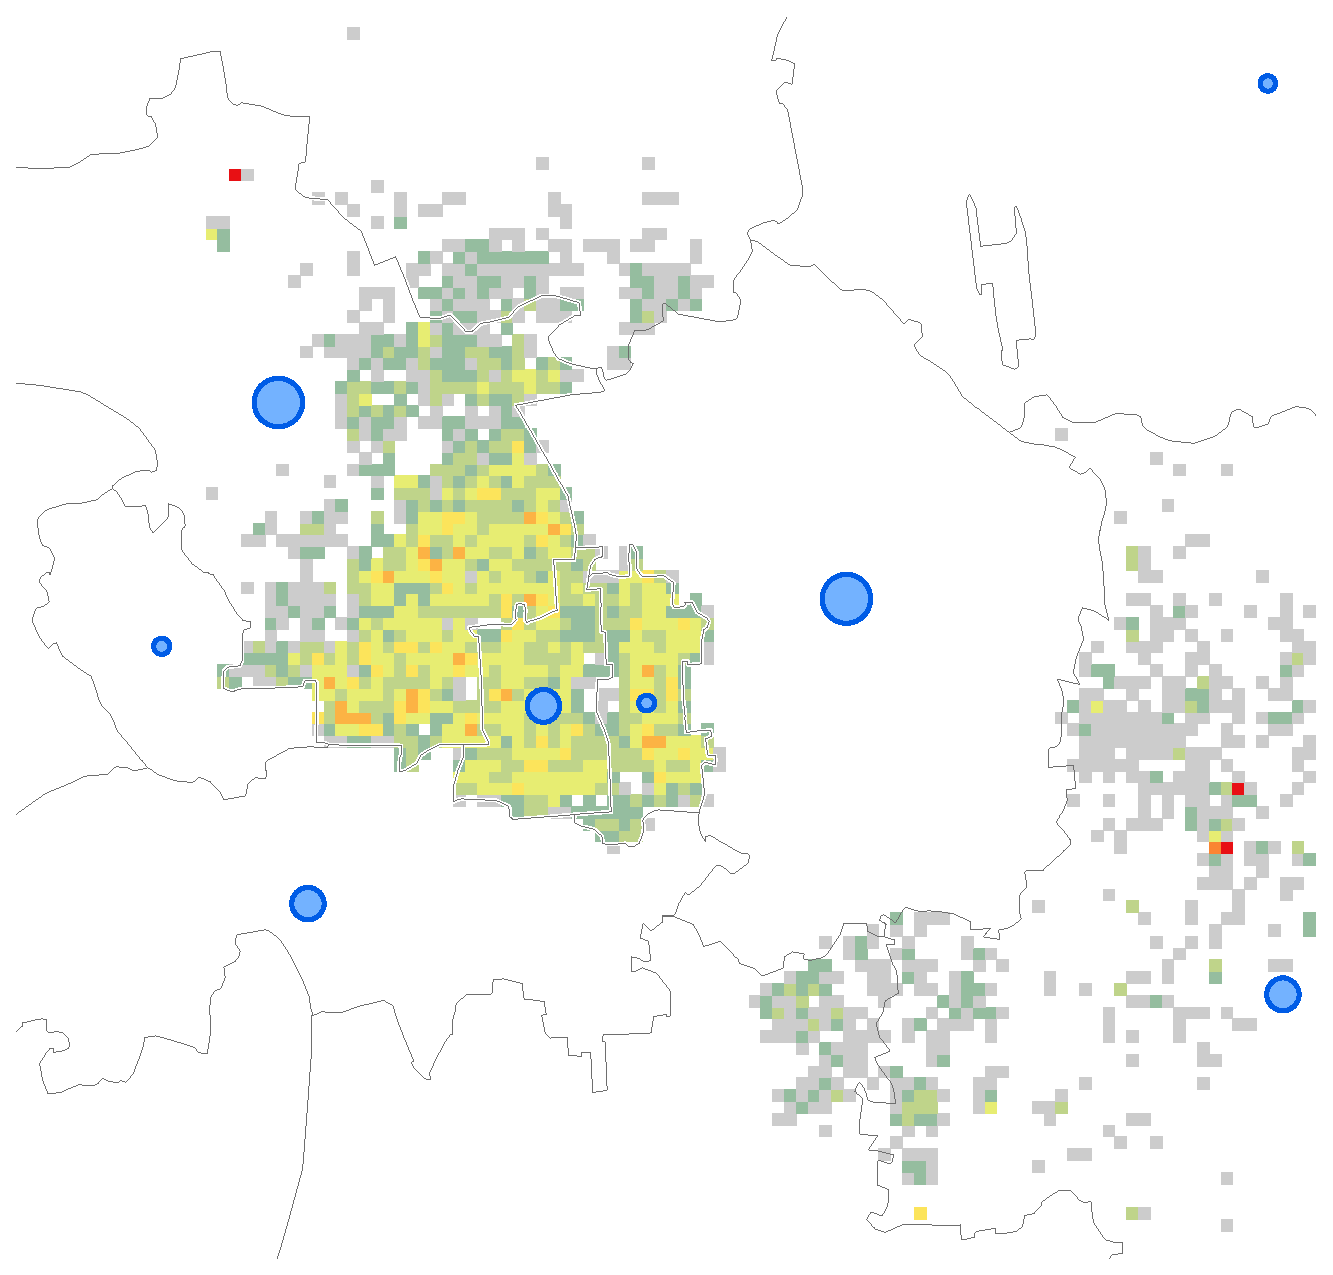
\includegraphics[width=\textwidth]{Figures/Relation_with_confrimed_cases/NewDistrictSSBD2020_01_30.eps}
        \caption{30 Jan}
    \end{subfigure}

    \vspace{6pt}
    \begin{subfigure}{.3\textwidth}
        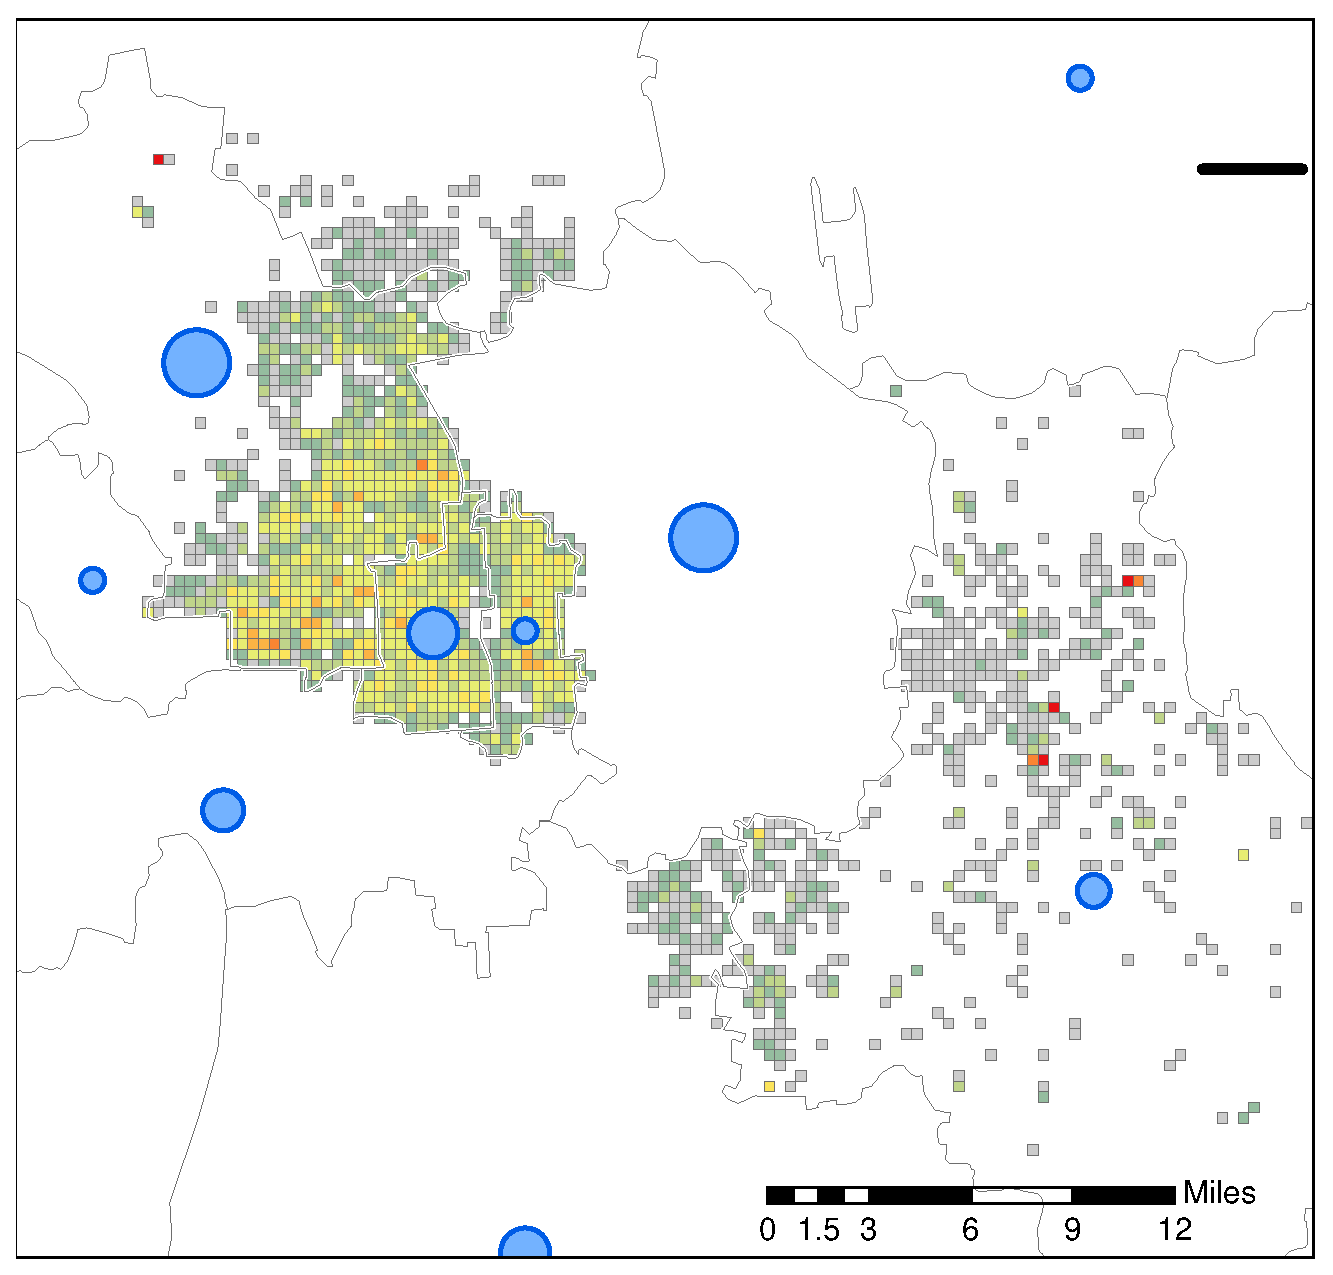
\includegraphics[width=\textwidth]{Figures/Relation_with_confrimed_cases/NewDistrictSSBD2020_02_04.eps}
        \caption{04 Feb}
    \end{subfigure}
    \begin{subfigure}{.3\textwidth}
        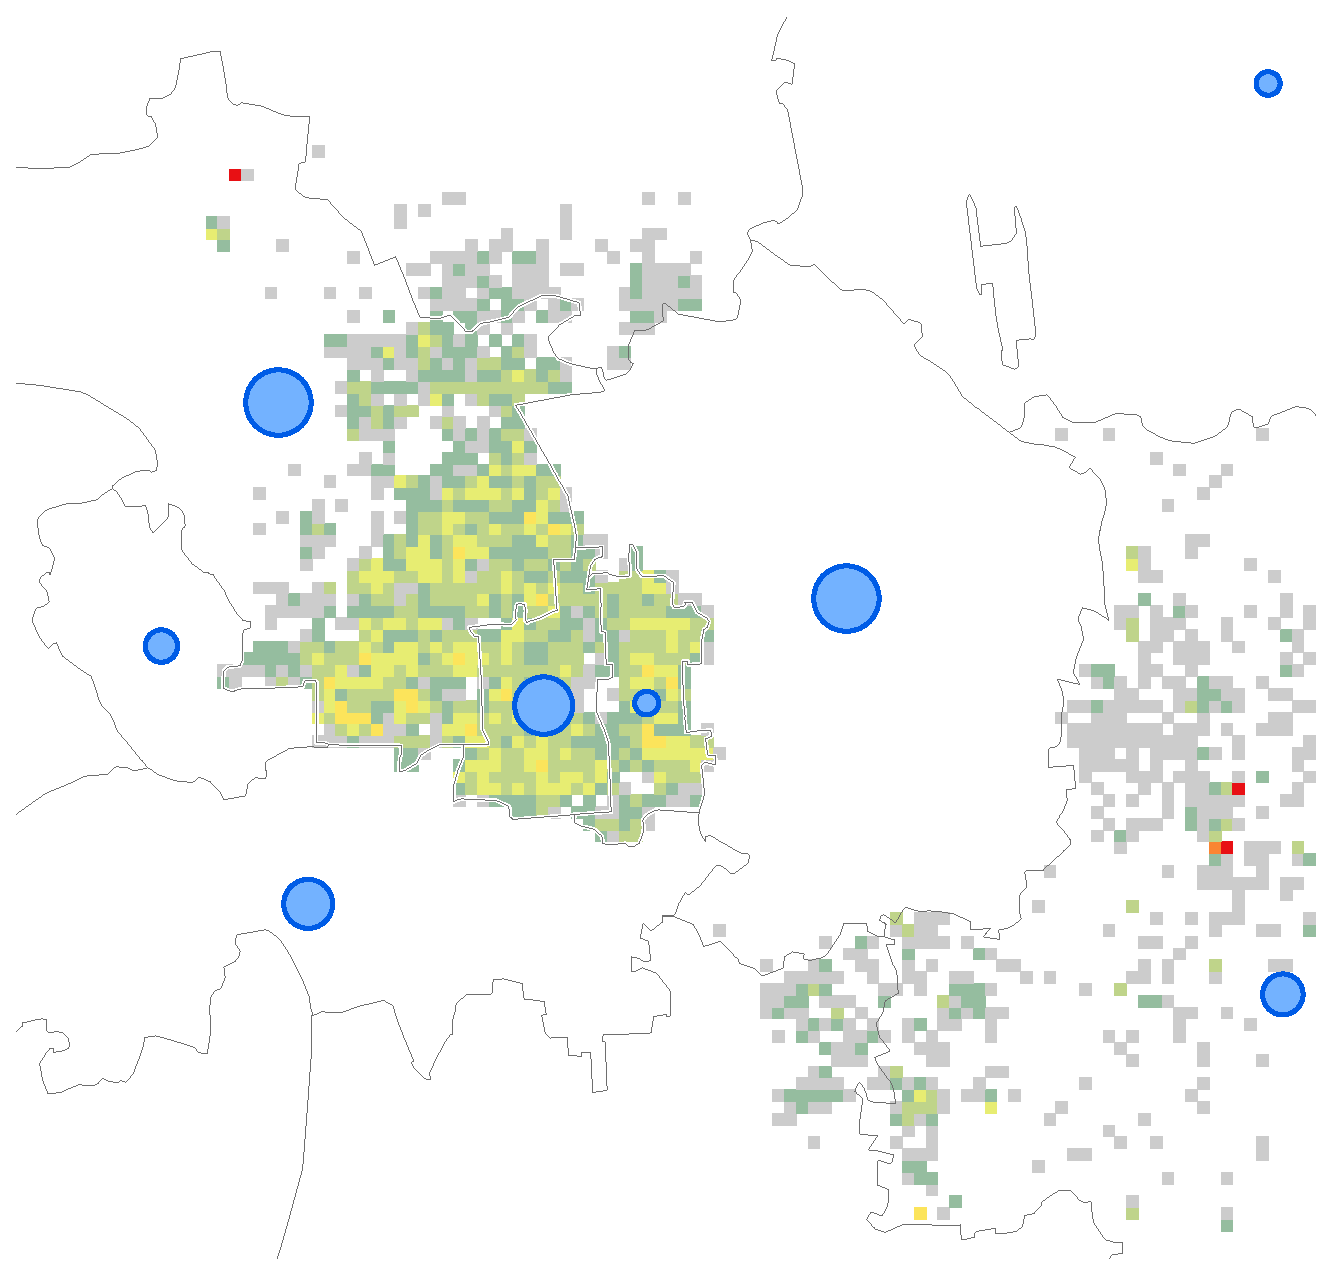
\includegraphics[width=\textwidth]{Figures/Relation_with_confrimed_cases/NewDistrictSSBD2020_02_08.eps}
        \caption{08 Feb}
    \end{subfigure}
    \begin{subfigure}{.3\textwidth}
        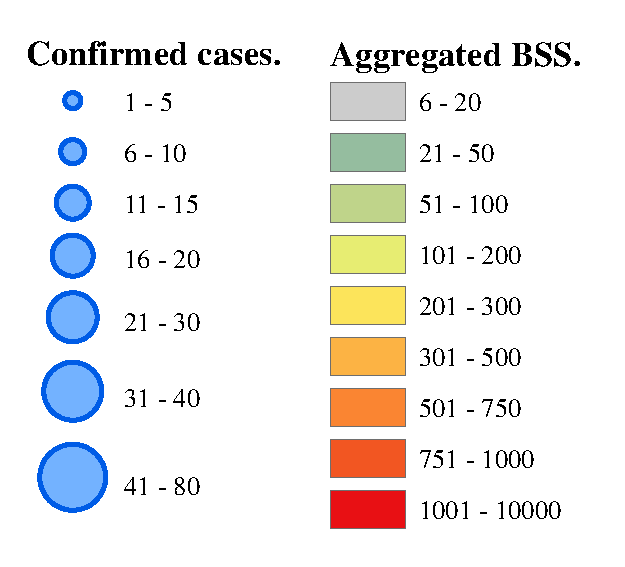
\includegraphics[width=\textwidth]{Figures/Relation_with_confrimed_cases/legend7.eps}
        \caption{legend}
    \end{subfigure}
    \caption{Relationships between cycling activities and confirmed cases during the quarantine period.}
    \label{fig:BSS_phase1_2}
\end{figure}

Figure \ref{fig:BSS_phase_3} depicts the share bike usages in \textbf{phase c}, when productive and social activities were allowed to restart partially.
%aim to identify and characterize disease-spreading human interactions, thus allowing authorities to gradually lift the most restrictive measures with more precision and confidence.
During the period of epidemic mitigation, aggregated share bike usage gradually rebounded with stable accumulated confirmed cases, which can be inferred from panel (a) - (c).
The recovery of city is unbalanced in the spatial domain.
An increase is observed in the urban districts, wheras changes are not significant in other areas.
A reduction in mobility on weekends could be inferred from comparison between panel (d) and (e), which was attributed to the awareness of the risk of infection of residents.
It should be highlighted that the accumulated confirmed cases stay substantially stable across this period, suggesting control measures were effective and necessary in the containment of the spread of COVID-19 during the resilience of Beijing.

\textcolor{red}{After the epidemic is effectively mitigated, cycling activities increased due to the rework requirements, which can be inferred from visualization. The difference is obvious comparing weekday and weekend.}

\begin{figure}[ht]
    \centering
    \begin{subfigure}{.3\textwidth}
        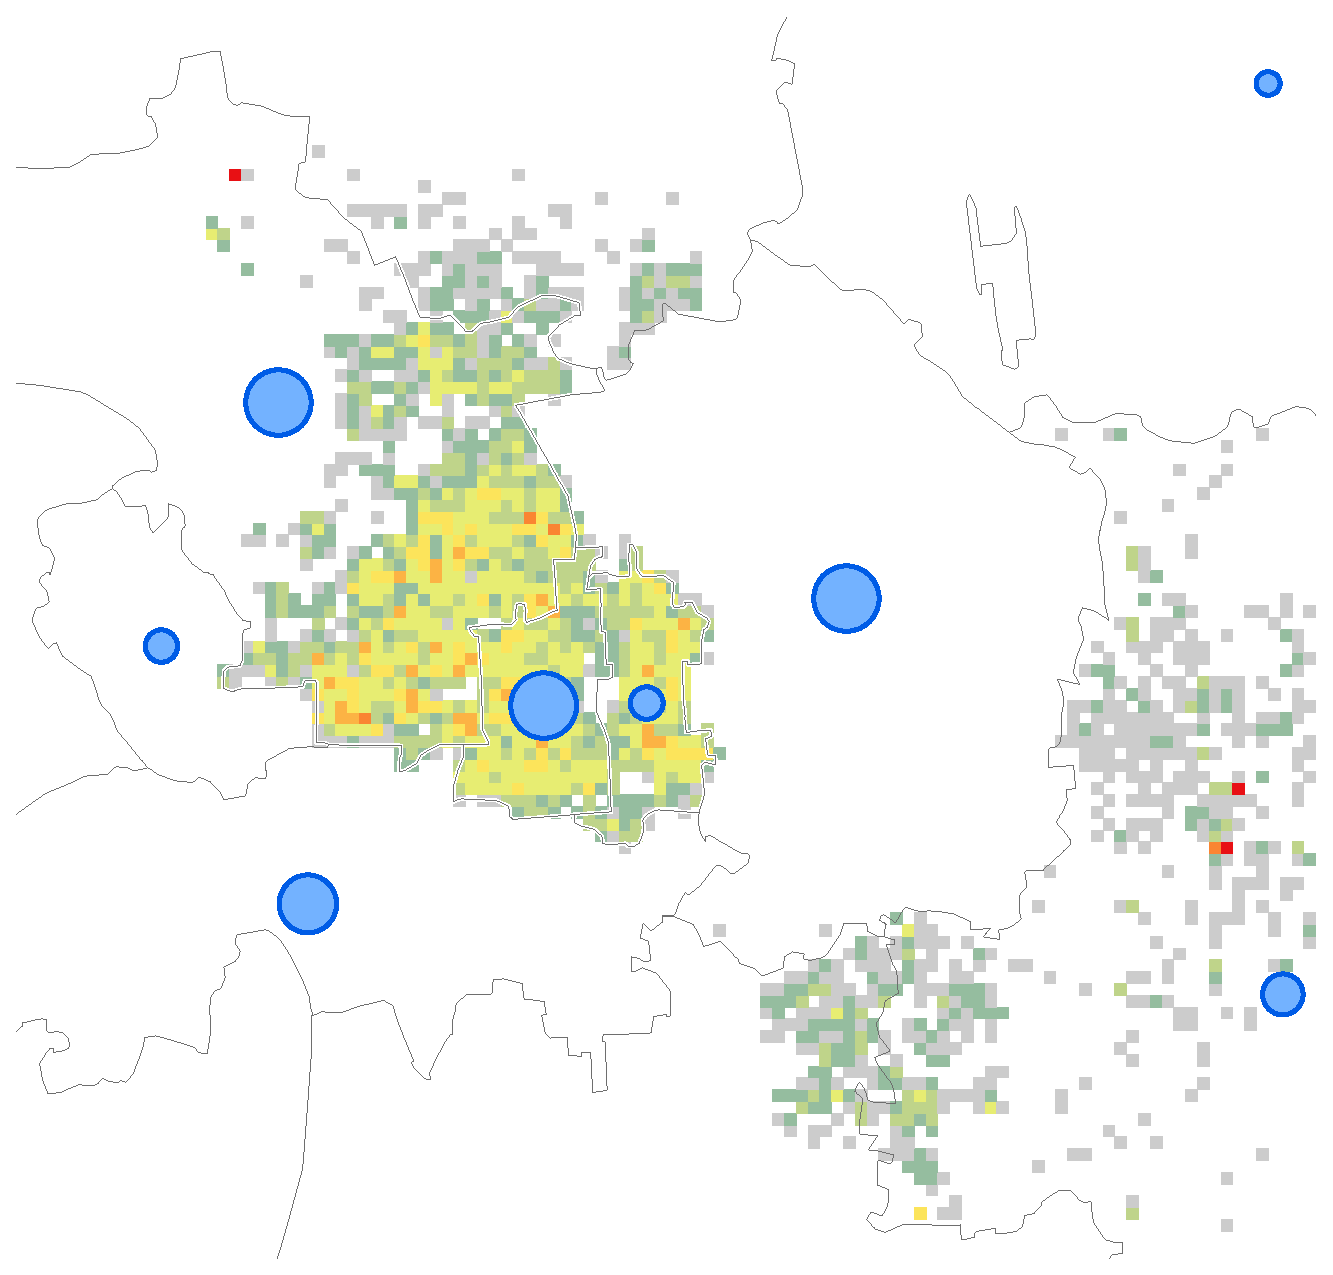
\includegraphics[width=\textwidth]{Figures/Relation_with_confrimed_cases/NewDistrictSSBD2020_02_12.eps}
        \caption{12 Feb}
    \end{subfigure}
    \begin{subfigure}{.3\textwidth}
        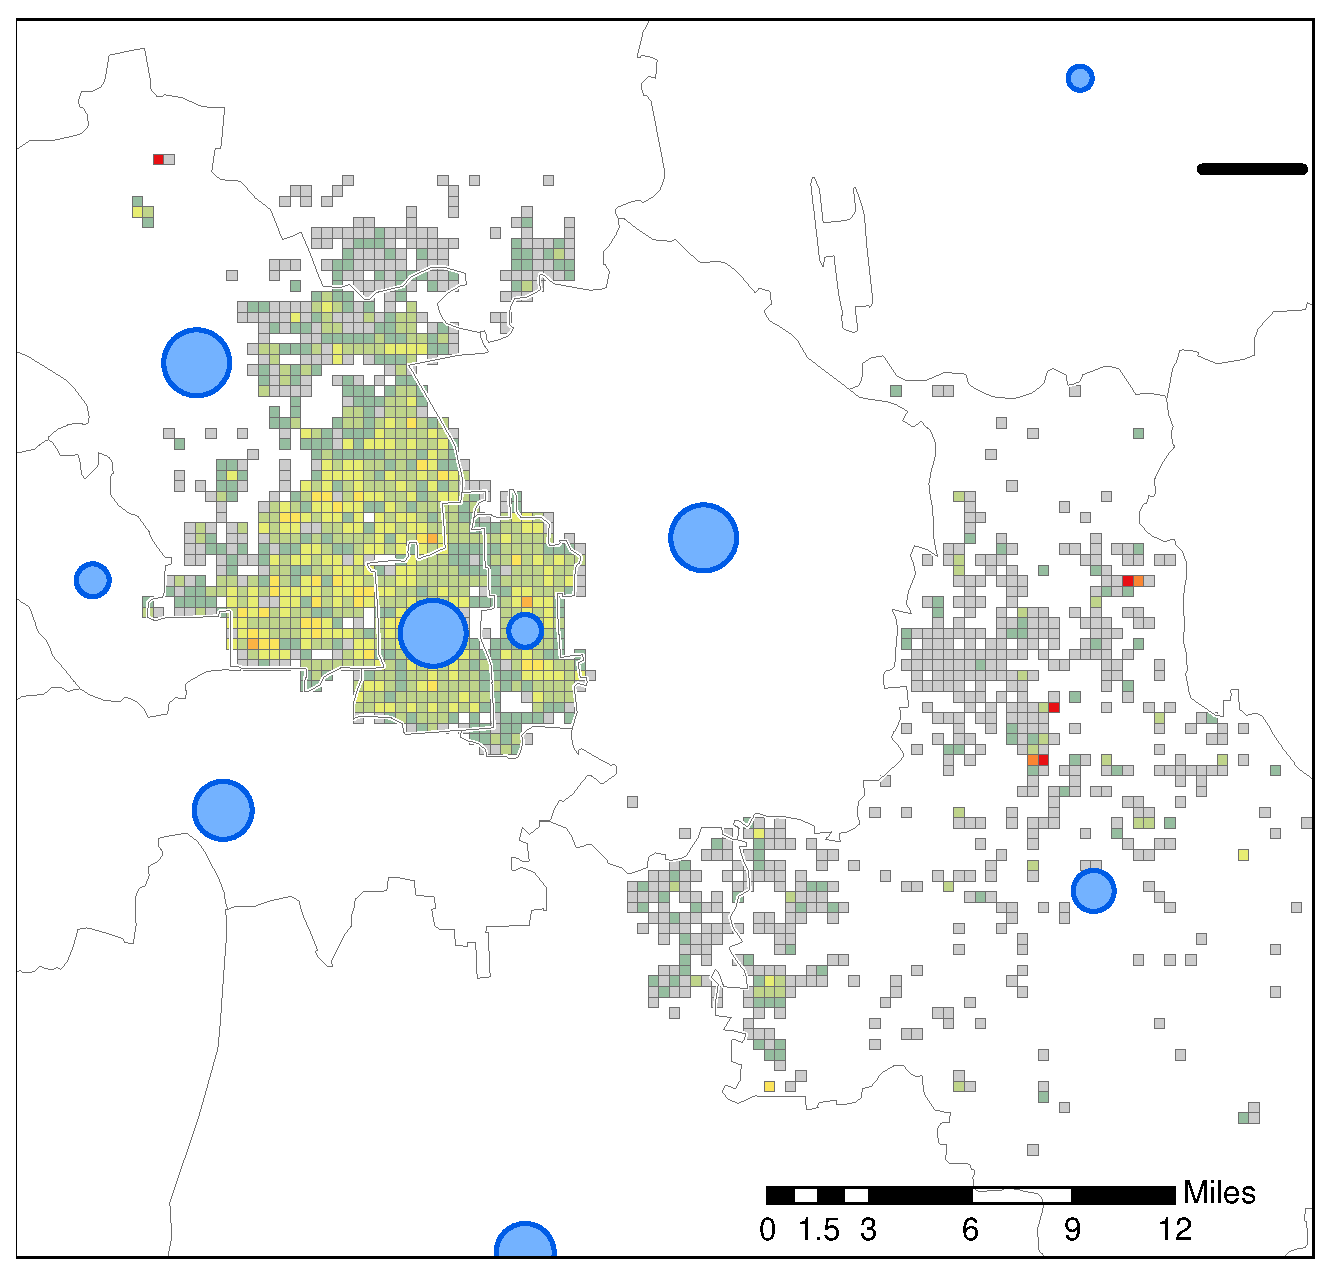
\includegraphics[width=\textwidth]{Figures/Relation_with_confrimed_cases/NewDistrictSSBD2020_02_16.eps}
        \caption{16 Feb}
    \end{subfigure}
    \begin{subfigure}{.3\textwidth}
        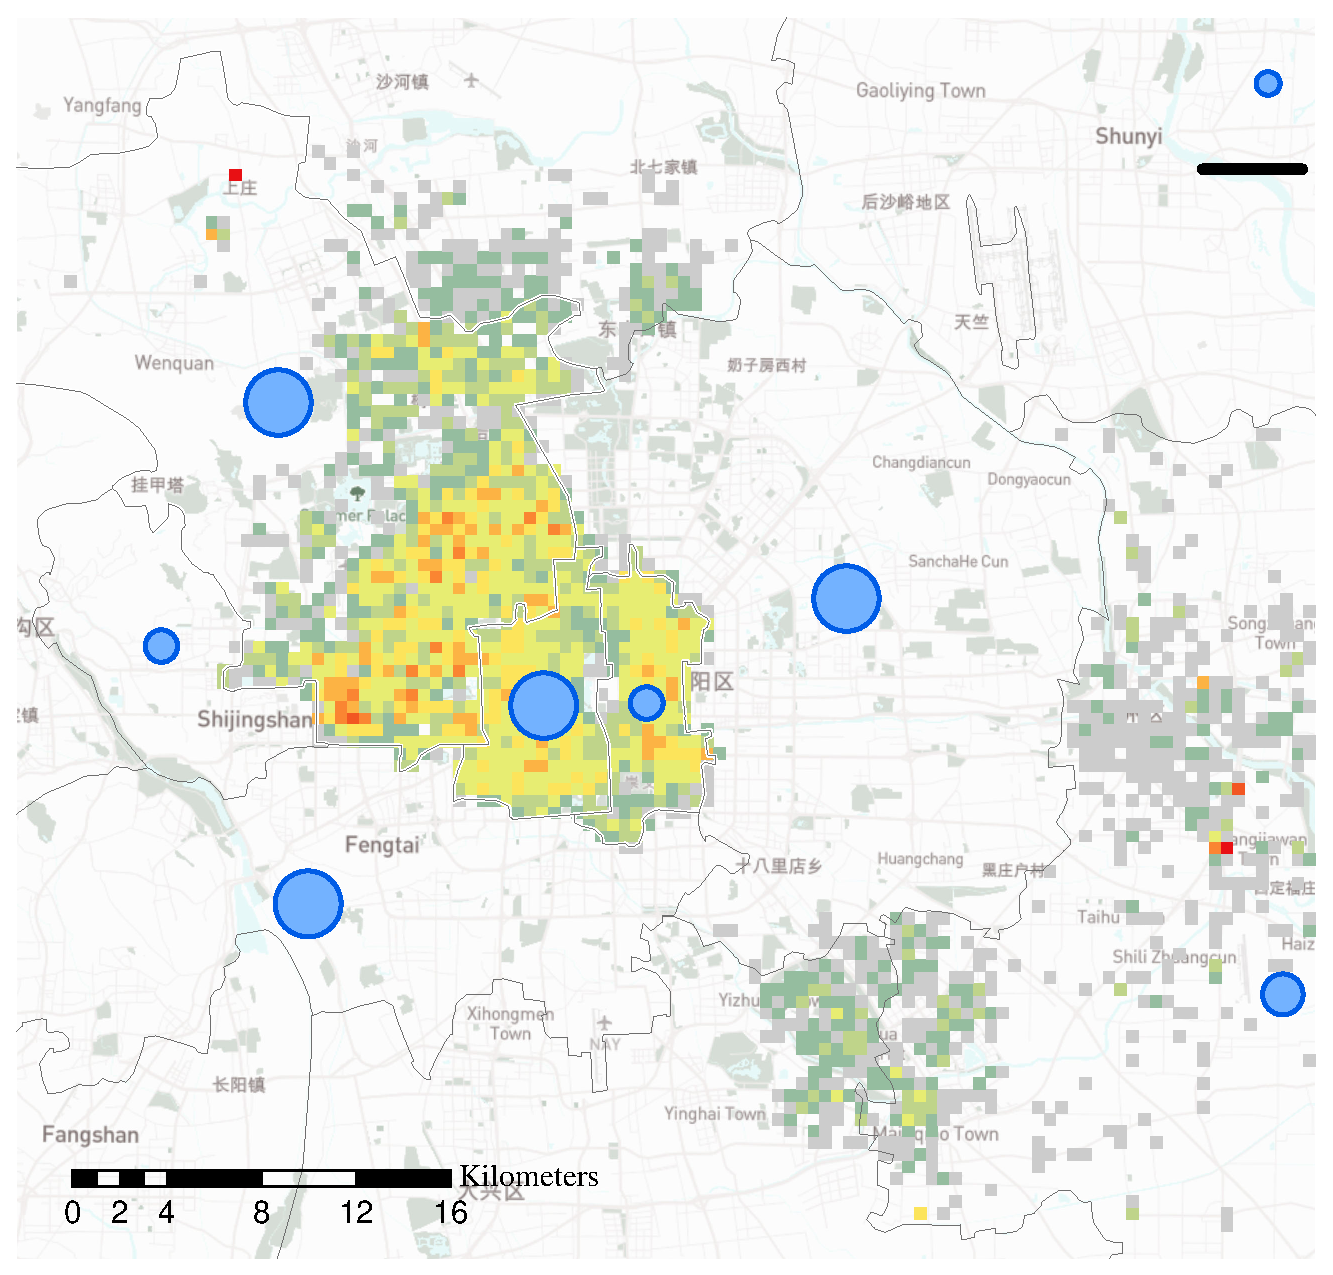
\includegraphics[width=\textwidth]{Figures/Relation_with_confrimed_cases/NewDistrictSSBD2020_02_20.eps}
        \caption{20 Feb}
    \end{subfigure}
    
    \vspace{6pt}
    \begin{subfigure}{.3\textwidth}
        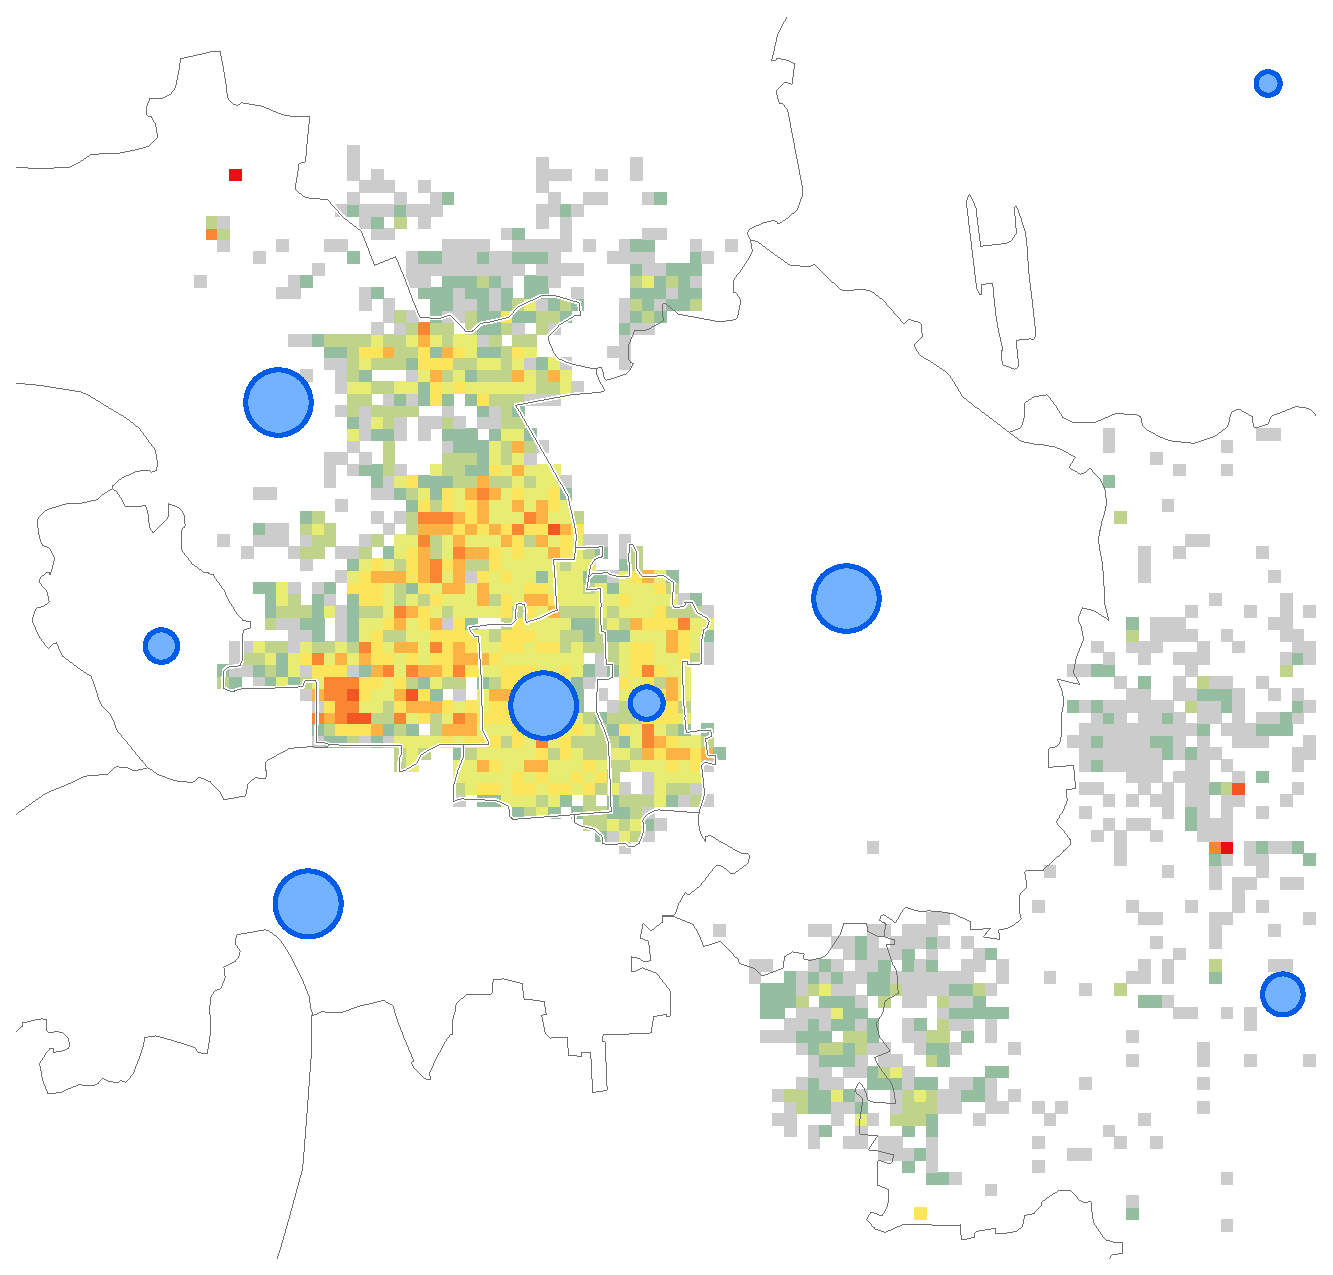
\includegraphics[width=\textwidth]{Figures/Relation_with_confrimed_cases/NewDistrictSSBD2020_02_24.eps}
        \caption{24 Feb}
    \end{subfigure}
    \begin{subfigure}{.3\textwidth}
        \includegraphics[width=\textwidth]{Figures/Relation_with_confrimed_cases/NewDistrictSSBD2020_02_28.eps}
        \caption{28 Feb}
    \end{subfigure}
    \begin{subfigure}{.3\textwidth}
        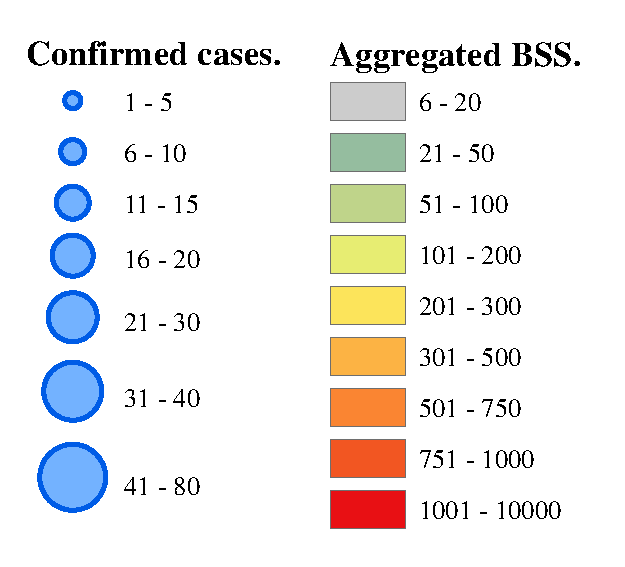
\includegraphics[width=\textwidth]{Figures/Relation_with_confrimed_cases/legend7.eps}
        \caption{legend}
    \end{subfigure}
    \caption{Relationships between cycling activities and confirmed cases when the epidemic is mitigated.}
    \label{fig:BSS_phase_3}
\end{figure}

%%%%%%%%%%%%%%%%%%%%%%%%%%%%%%%%%%%%%%%%%%%%%%


\section{Conclusion}

Motivated by the current COVID-19 outbreak and rapid development in BSS, this paper reveals the period-wise spatiotemporal patterns and co-location patterns of the share bike usage before \& during the pandemic in Beijing, China.
We investigated the impact of the pandemic on the mobility of individuals and the rehabilitation process of Beijing.
By removing the factor of Chinese New Year holiday, social and productive activities of residents were hugely affected by the COVID-19, reflected in the drastic decrease of share bike usage (down to less than $40\%$ of that of the same period in 2019). 
The cumulative confirmed cases stayed stable substantially after restarting of productive activities, indicating the control measures were necessary and effective in containment of the spread of COVID-19 when opening-up.
%TODO co-location的结果显示几种POI在疫情阶段的访问情况。
Co-location analyis shows the infected RAs situated in the city center are mostly impacted, even after the pandemic is mitigated;
Among POIs, share bike usage of tech companies has the biggest change before and during the pandemic as these companies are most suitable for ``work from home'', \textit{etc}.

These results are references to epidemiological researches and inform policy making in the context of the current COVID-19 outbreak, and help to prevent the emergence of pandemics in the future.
However, the government implemented multiple interventions at the same time or in a short timeframe to control the outbreak, therefore individual strategies could not be evaluated.
Correlation analysis was performed based on confirmed cases data extracted from the infectious disease reporting system. 
With additional information concerning epidemiological characteristics, spatiotemporal epidemic model is planned to predict the spread of pandemic in the future.

\section{Future Work}

Our current work has extracted the features of mobility reflected by BSS.
A possible extension is to build a dynamic model based on the features predicting the share bike usage and potential social event/reaction of public during the pandemic or emergencies.

%%%%%%%%%%%%%%%%%%%%%%%%%%%%%%%%%%%%%%%%%%
\vspace{6pt} 

%%%%%%%%%%%%%%%%%%%%%%%%%%%%%%%%%%%%%%%%%%
%% optional
%\supplementary{The following are available online at \linksupplementary{s1}, Figure S1: title, Table S1: title, Video S1: title.}

%%%%%%%%%%%%%%%%%%%%%%%%%%%%%%%%%%%%%%%%%%
%% optional
\abbreviations{The following abbreviations are used in this manuscript:

\noindent 
\begin{tabular}{@{}ll}
GIS & Geographic Information System \\
BSS & Bike Sharing System\\
POI & Point Of Interest \\
RA & Residential Area

\end{tabular}}

%%%%%%%%%%%%%%%%%%%%%%%%%%%%%%%%%%%%%%%%%%
%% optional

\newpage
\appendixtitles{no} %Leave argument "no" if all appendix headings stay EMPTY (then no dot is printed after "Appendix A"). If the appendix sections contain a heading then change the argument to "yes".
\appendix
\section{Figures Illustrating Colocation Patterns with POIs}

% \textcolor{red}{Visualization and analysis on RAs and BSS usage with respect to epidemic period.}

\begin{figure}[ht]
    \centering
    \begin{subfigure}{.334\textwidth}
        \includegraphics[width=\textwidth]{Figures/Relation_with_POIs/POI_resD2020_01_25.eps}
        \caption{25 Jan}
    \end{subfigure}
    \begin{subfigure}{.334\textwidth}
        \includegraphics[width=\textwidth]{Figures/Relation_with_POIs/POI_resD2020_02_09.eps}
        \caption{09 Feb}
    \end{subfigure}

    \vspace{6pt}
    \begin{subfigure}{.334\textwidth}
        \includegraphics[width=\textwidth]{Figures/Relation_with_POIs/POI_resD2020_02_18.eps}
        \caption{18 Feb}
    \end{subfigure}
        \begin{subfigure}{.334\textwidth}
        \includegraphics[width=\textwidth]{Figures/Relation_with_POIs/POI_resD2020_03_02.eps}
        \caption{02 Mar}
    \end{subfigure}
    \caption{BSS and communities.}
    \label{fig:BSS_communities}
\end{figure}

% \textcolor{red}{Visualization and analysis on traffic/metro and BSS usage with respect to epidemic period.}

\begin{figure}[ht]
    \centering
    \begin{subfigure}{.334\textwidth}
        \includegraphics[width=\textwidth]{Figures/Relation_with_POIs/POI_metroD2020_01_25.eps}
        \caption{25 Jan}
    \end{subfigure}
    \begin{subfigure}{.334\textwidth}
        \includegraphics[width=\textwidth]{Figures/Relation_with_POIs/POI_metroD2020_02_09.eps}
        \caption{09 Feb}
    \end{subfigure}

    \vspace{6pt}
    \begin{subfigure}{.334\textwidth}
        \includegraphics[width=\textwidth]{Figures/Relation_with_POIs/POI_metroD2020_02_18.eps}
        \caption{18 Feb}
    \end{subfigure}
        \begin{subfigure}{.334\textwidth}
        \includegraphics[width=\textwidth]{Figures/Relation_with_POIs/POI_metroD2020_03_02.eps}
        \caption{02 Mar}
    \end{subfigure}
    \caption{BSS and metro.}
    \label{fig:BSS_metro}
\end{figure}

% \textcolor{red}{Visualization and analysis on malls and BSS usage with respect to epidemic period.}
\clearpage

\begin{figure}[ht]
    \centering
    \begin{subfigure}{.334\textwidth}
        \includegraphics[width=\textwidth]{Figures/Relation_with_POIs/POI_mallsD2020_01_25.eps}
        \caption{25 Jan}
    \end{subfigure}
    \begin{subfigure}{.334\textwidth}
        \includegraphics[width=\textwidth]{Figures/Relation_with_POIs/POI_mallsD2020_02_09.eps}
        \caption{09 Feb}
    \end{subfigure}

    \vspace{6pt}
    \begin{subfigure}{.334\textwidth}
        \includegraphics[width=\textwidth]{Figures/Relation_with_POIs/POI_mallsD2020_02_18.eps}
        \caption{18 Feb}
    \end{subfigure}
    \begin{subfigure}{.334\textwidth}
        \includegraphics[width=\textwidth]{Figures/Relation_with_POIs/POI_mallsD2020_03_02.eps}
        \caption{02 Mar}
    \end{subfigure}
    \caption{BSS and malls.}
    \label{fig:BSS_malls}
\end{figure}

% \textcolor{red}{Visualization and analysis on companies and BSS usage with respect to epidemic period.}

\begin{figure}[ht]
    \centering
    \begin{subfigure}{.334\textwidth}
        \includegraphics[width=\textwidth]{Figures/Relation_with_POIs/POI_compD2020_01_25.eps}
        \caption{25 Jan}
    \end{subfigure}
    \begin{subfigure}{.334\textwidth}
        \includegraphics[width=\textwidth]{Figures/Relation_with_POIs/POI_compD2020_02_09.eps}
        \caption{09 Feb}
    \end{subfigure}

    \vspace{6pt}
    \begin{subfigure}{.334\textwidth}
        \includegraphics[width=\textwidth]{Figures/Relation_with_POIs/POI_compD2020_02_18.eps}
        \caption{18 Feb}
    \end{subfigure}
        \begin{subfigure}{.334\textwidth}
        \includegraphics[width=\textwidth]{Figures/Relation_with_POIs/POI_compD2020_03_02.eps}
        \caption{02 Mar}
    \end{subfigure}
    \caption{BSS and companies.}
    \label{fig:BSS_companies}
\end{figure}

%%%%%%%%%%%%%%%%%%%%%%%%%%%%%%%%%%%%%%%%%%


\reftitle{References}

\externalbibliography{yes}
\bibliography{bib}

%%%%%%%%%%%%%%%%%%%%%%%%%%%%%%%%%%%%%%%%%%
%% optional
% \sampleavailability{Samples of the compounds ...... are available from the authors.}

%% for journal Sci
%\reviewreports{\\
%Reviewer 1 comments and authors’ response\\
%Reviewer 2 comments and authors’ response\\
%Reviewer 3 comments and authors’ response
%}

%%%%%%%%%%%%%%%%%%%%%%%%%%%%%%%%%%%%%%%%%%
\end{document}

